\bookpart{信息与奖励受限的学习}{Learning with Limited Information and Reward}
\label{part:rl-information-and-reward}

\BookPartGuide{%
导航策略可能只取得局部相机观测，也可能只能使用过去保存的交互记录；即使允许继续行动，奖励也可能在任务结束时才出现，或只能由人工比较间接提供。这些限制作用于不同环节：观测决定行动前能够区分哪些状态，训练记录决定能够从哪些行为后果估计候选策略的价值，奖励则决定学习依据能否反映预定目标。本部分在前述规划与交互学习的共同设定上，分别研究这些限制。

第~\ref{chap:rl-information}章“信息受限下的强化学习”区分两类问题。状态不能完整观测时，需要由观测、过去动作及已见奖励形成可供决策的历史表示，或维护对可能状态的概率判断（信念）；交互记录固定时，则要检查行为策略的覆盖范围，判断候选策略的价值能否由现有训练样本确定，再讨论保守估计与受限的策略改进。两类限制同时出现时，历史表示能够预测后续观测，并不自动说明它足以评价未执行的动作。

第~\ref{chap:rl-reward}章“奖励受限下的强化学习”分别处理奖励难以观察、长期奖励难以归因和奖励与行为目标不匹配的问题。示范、偏好与可验证反馈提供不同的训练依据；奖励塑形、辅助任务和反馈模型改变学习信号，却各自需要检查策略是否仍然追求原定目标。新的策略产生新的交互记录后，还要重新核对反馈模型及其适用范围。

两章共同区分能否确定待估对象、有限训练样本下估计有多准确，以及已有学习规则能否求得合适策略。增加历史表示、补充训练记录或改变奖励反馈，解决的是其中不同的缺口；结论所需的覆盖、可识别性和目标一致性条件仍须分别成立。}


\chapter{信息受限下的强化学习}
\label{chap:rl-information}

一辆小车驶近岔路口，摄像头清楚地拍到了它的位置，控制器仍可能无法决定怎样转向。如果画面没有显示小车向哪一侧滑动，控制器需要借助过去的观测辨认当前运动状态。如果位置和速度都已知，但日志从未记录某种转向动作，学习者需要判断现有经验能否说明该动作的后果。前一种困难缺少用于辨认当前状态的观测线索，后一种缺少备选行动的后果证据。过去的观测可能帮助估计速度，但未必能精确恢复所有隐藏状态；记忆本身也不能告诉我们一个从未尝试的转向会怎样。反复训练可以重新利用日志，却不能把未记录的线索或未发生的试验变成已知事实。

第~\ref{chap:rl-learning}~章已经说明怎样从经验估计价值、优化策略和学习模型。本章考察这些方法在状态不全可见或只能使用固定日志时还能使用到哪一步。状态不可见时，我们要从当前观测转向完整历史，或构造保留动作后果预测依据的历史表示。经验固定时，首先要检查同一批可见记录是否仍允许两种不同的环境解释。例如，一个解释认为未试过的左转更好，另一个认为它更差；若两者都符合采集规律，日志本身就不能确定左转的价值。排除这种答案不唯一的困难以后，才有依据讨论基于有限训练记录的价值估计和策略改进。图~\ref{fig:rl-information-roadmap}~将这两条认识路径分开。离线部分可观测问题同时受到两类限制：既要检查历史中留下了哪些线索，也要检查收集者依据什么选择了日志中的动作。

本章先沿这两条路径分别推演，再检查它们同时存在时的条件。状态不全的路径从已有历史出发，研究怎样压缩、更新并用于动作比较；固定日志的路径从收集机制出发，研究哪些价值能确定、怎样估计，以及生成新策略时如何防止利用外推错误。允许少量新试验会改变证据来源，因此单独讨论其作用。所需概率计算主要是条件概率、加权平均和期望；新的识别条件会在对应问题中说明。

\begin{figure*}[htbp]
  \centering
  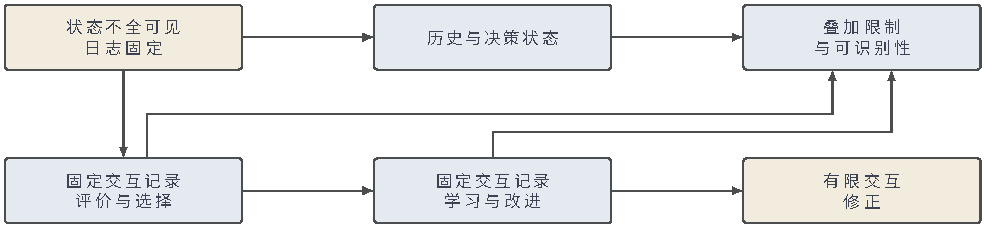
\includegraphics[width=166.857mm]{figures/10-reinforcement-learning/02-information-and-reward/tikz/rl-information-roadmap.pdf}
  \caption{本章的阅读依赖。箭头表示理解后项需要前项建立的概念，不表示算法的执行顺序。历史表示说明行动时能依据什么，固定日志上的策略评价说明已有经验能支持哪些判断；两者共同限制离线部分可观测问题中的策略结论。}
  \label{fig:rl-information-roadmap}
\end{figure*}

% Outline: 4.1
\Needspace{6\baselineskip}
\section{两类信息限制}
\label{sec:rl-information-limits}

% Outline: 4.1.1
\subsection{决策所依据的状态信息}
\label{sec:rl-information-state-information}

第~\ref{chap:rl-overview}~章的马尔可夫条件针对完整状态$s_t$：给定它和当前动作，就能描述下一步的条件分布，无须再查询更早的经历。摄像头取得的$o_t$只显示位置，未直接给出速度，给定同一画面和动作，后果仍可能随未见的速度而变化。因此，执行策略不能沿用直接依据$s_t$决策的规则，而要考虑此前已取得的记录。一步记录$(o_t,a_t,r_t,o_{t+1})$按真实交互时刻$t$排列：先看到$o_t$，再执行$a_t$，随后取得奖励$r_t$和下一观测。这个时间下标不表示训练中的梯度更新次数。

过去动作也应进入历史，因为同一对画面可以由不同控制输入产生。例如，看到小车位置没有改变，既可能是未施加动力，也可能是施力后遇到障碍；只存画面会把这两种经历合并。我们因此把每一步已经看见、已经执行、已经收到的内容按发生顺序一起保存，作为当前策略真正能读取的材料。

历史中也保留奖励，因为奖励可能帮助辨认状态。例如，碰撞后返回的奖励可以说明小车触及了画面中看不见的障碍；删去它，就可能丢掉下一次决策需要的线索。这里保留的都是已经发生的反馈，未来才揭示的状态或奖励不能提前交给当前策略。

\begin{definition}[决策历史]
  \label{def:rl-information-history}
  时刻$t$的完整记录历史按时间排列行动前已经取得的观测、动作和奖励，写为
  \[
    I_t=(o_0,a_0,r_0,\ldots,a_{t-1},r_{t-1},o_t).
  \]
  历史条件策略$\pi(a\mid I_t)$以行动前已获得的观测、动作和奖励为依据。当前观测策略仅依据$o_t$决策；长度为$L$的窗口策略仅保留最近$L$步记录，并须约定窗口在回合边界处怎样构造。
\end{definition}

\begin{example}[相同位置与不同记忆]
  \label{ex:rl-information-cue}
  考虑一个独立教学任务。小车的真实状态包括位置$x_t$和速度$v_t$，摄像头只给出位置。同样看到$x_t=0$时，若$v_t=1$，所需制动方向与$v_t=-1$时相反。为判断运动方向，可以比较相邻位置。在无噪声、采样间隔为1且速度在相邻采样间不变的简化条件下，$v_t=x_t-x_{t-1}$；两次位置观测足以恢复速度，单帧不能给出这个位移差。

  再考虑线索出现得更早的岔路任务。回合开始时，提示$c\in\{L,R\}$以相同概率显示；小车随后经过$L+1$步外观相同的走廊，途中只能前进，奖励均为0。出口处选中$c$指示的方向得1，选错得0。本例及后文均按不折扣的回合成功奖励比较，其期望就是成功概率，不采用默认折扣回报。完整历史策略可以记住提示，期望成功奖励达到1。最近$L$步窗口已经看不到提示，固定的前进动作也不能编码提示，因此这类策略的最好期望成功奖励为$1/2$。
\end{example}

在岔路任务中，窗口内的观测、动作和奖励记录对左右提示完全相同。任何只读该窗口的策略都只能给出同一动作概率：设它以概率$p$选左，成功概率为$(1/2)p+(1/2)(1-p)=1/2$。这个结果不取决于网络有多大，也不取决于$p$怎样训练；被删除的提示根本没有进入策略可读取的记录。保留一位左右记忆就足够，而不断重复读取相同走廊画面不提供新的左右提示。

位置任务只需多保留一帧，便能补出缺失的速度；岔路任务却说明，任意预先固定的窗口都可能因线索延迟更长而失效。表示是否足够，取决于它有没有保留能区分候选动作后果的观测、动作和奖励记录，而不是保留的历史记录序列单纯有多长。

% Outline: 4.1.2
\subsection{学习能够访问的经验}
\label{sec:rl-information-data-access}

现在让日志完整记录小车的位置和速度。如果收集者在某个状态从不向左转，我们仍可能不知道在那里左转会怎样。缺口不在单条记录的字段，而在整批记录涉及的行为。分析可用经验时，必须分别检查记录是否完整、收集行为覆盖了哪里，以及学习者能否主动补采样。

固定日志下，学习者可以重新抽取记录、计算梯度、拟合价值或模型，但这些操作的结果都依赖同一批原始证据。允许新交互时则不同：学习者可以真实执行过去没有尝试的动作，并看到它的结果。为比较这两种学习条件，需要把算法能算什么与算法能查询什么分开；下面的协议规定的是后者，包括用于选模或评价的真实调用。

\begin{definition}[经验访问协议]
  \label{def:rl-information-access}
  \term{固定经验}协议将可用材料限定为给定的有限交互记录组$D$及声明可用的采集元数据，训练和选模期间都不允许查询真实环境。\term{有限新增交互}协议允许在约定的轮次和预算内补充真实经验；每轮可执行的策略、重置权限和专家帮助权限均由协议规定。\term{持续在线交互}协议允许策略根据经验不断更新并继续采集交互训练记录，但重置、传感和测试权限仍须明确，不能据此假定可以从任意状态采样。
\end{definition}

固定日志即使回放一百万轮，真实访问过的状态和动作也不会增加，改变的只是算法利用这些记录的方式。学习模型生成一百万条模拟转移，同样没有新增真实查询。表~\ref{tab:rl-information-access}~沿用完整记录位置和速度的小车任务，对照交互权限改变后能够取得的证据。

\begin{table*}[htbp]
  \centering
  \small
  \begin{tabularx}{\linewidth}{p{20mm}XXXX}
    \toprule
    协议 & 记录字段 & 行为覆盖 & 主动采样权限 & 评价查询权限 \\
    \midrule
    固定经验 & 位置、速度、动作、奖励和回合边界 & 仅原日志的收集行为 & 无真实调用、无重置 & 只能离线估计；不能试跑候选 \\
    有限新增 & 原字段加策略版本、轮次和查询用途 & 原日志加预算内新增行为 & 每轮限定步数；重置单列计数 & 允许的测试也扣除预算 \\
    持续在线 & 同样记录状态与行为元数据 & 随收集策略持续变化 & 在可达轨迹上继续行动；任意状态重置仍需授权 & 独立测试记录不参与拟合或选模，查询成本单列 \\
    \bottomrule
  \end{tabularx}
  \caption{同一完全可观测小车任务中的三种经验协议。完整字段不能补齐未尝试的动作；可以继续交互，也不意味着可以像调用生成模型那样从任意指定状态采样。}
  \label{tab:rl-information-access}
\end{table*}

% Outline: 4.1.3
\subsection{观测完整性与新增交互权限的组合}
\label{sec:rl-information-two-axes}

小车能否取得完整状态，并不决定训练者能否继续驾驶它。只见位置的控制器可以被允许主动加减速，借反馈辨认运动方向；已经记录位置和速度的日志也可以禁止新增试验。表~\ref{tab:rl-information-two-axes}~将观测完整性与交互权限交叉排列，得到四种条件。

\begin{table}[htbp]
  \centering
  \small
  \begin{tabularx}{\linewidth}{p{18mm}XX}
    \toprule
    执行观测 & 可新增真实交互 & 只有固定经验 \\
    \midrule
    完整状态 & 位置、速度均可见，可继续控制小车 & 状态字段完整，但只能使用已有驾驶日志 \\
    部分观测 & 只见位置，需要历史，可主动探查 & 只见位置，需要历史，仅有固定轨迹 \\
    \bottomrule
  \end{tabularx}
  \caption{观测完整性与训练记录采集权限可以交叉组合。允许少量新增经验只放宽访问权限，不改变观测类型；这些部分观测任务的模型将在下节建立。}
  \label{tab:rl-information-two-axes}
\end{table}

历史压缩遗漏线索与日志未覆盖目标动作会导致不同的失败。两类限制同时存在时，还要核对日志保存的历史与采集者选择动作的依据，不能把一种限制的处理直接用于另一种限制。

% Outline: 4.2
\section{决策信息不完整下的强化学习}
\label{sec:rl-information-partial-observation}

% Outline: 4.2.1
\subsection{从当前观测扩展为可得历史}
\label{sec:rl-information-history-policy}

回到例~\ref{ex:rl-information-cue}~的出口：同一画面下，早期提示为左时应向左，为右时应向右。\term{观测混叠}（observation aliasing）就是不同决策处境对应同一个当前观测，因而仅凭该观测无法区分它们。完整隐藏状态可以满足马尔可夫条件，观测过程却未必满足；我们需要同时描述状态怎样演化、观测怎样产生。图~\ref{fig:rl-information-aliasing}~将这两种关系分开，也显示相同当前观测可以来自不同历史。

前章用一个状态变量同时表达“环境当前处于哪里”和“策略现在知道什么”。这里要把二者分开。小车的完整状态含位置与速度，摄像头给出的读数却可能只有位置；同一位置读数对应多种完整状态，不能再直接用观测代替状态作Bellman备份。环境仍从完整状态出发演化，我们另给一条观测生成规律，说明这一演化的哪些结果能够被控制器看见。动作还可能改变观测方式，如停下观察或主动倾听，因此反馈模型要保留动作条件。

\begin{definition}[有限部分可观测马尔可夫决策过程]
  \label{def:rl-information-pomdp}
  \term{部分可观测马尔可夫决策过程}（partially observable Markov decision process, POMDP）分别描述环境的隐藏状态和智能体取得的观测。设$S$、$\mathsf A$、$\mathsf O$分别为有限非空状态集、动作集和观测集，$\mu_0$为$S$上的初始分布，$H$为正整数时域；奖励取值于有限非空集$\mathcal R\subset\mathbb R$。

  初始观测核$K_{o,0}:S\to\Delta(\mathsf O)$在$s_0\sim\mu_0$后生成$o_0$。时刻$t=0,\ldots,H-1$，策略依据$I_t$选择$a_t$，环境随后生成$s_{t+1}$及反馈$y_{t+1}=(r_t,o_{t+1})$。令$\mathcal Y=\mathcal R\times\mathsf O$，将下一状态与反馈的条件分布合写为联合概率核$K:S\times\mathsf A\to\Delta(S\times\mathcal Y)$；对每个$(s,a)$，$K(s',y\mid s,a)\geq0$且$\sum_{s',y}K(s',y\mid s,a)=1$。其生成含义为
  \[
    K(s',y\mid s,a)
    =\mathbb P(s_{t+1}=s',y_{t+1}=y\mid s_t=s,a_t=a).
  \]
  对反馈求和得到转移核$T(s'\mid s,a)=\sum_yK(s',y\mid s,a)$；按奖励值加权所有后果，得到期望奖励
  $R(s,a)=\sum_{s',r,o'}rK(s',(r,o')\mid s,a)$。奖励有界，采用回报
  $\sum_{t=0}^{H-1}\gamma^t r_t$，其中$0\leq\gamma<1$，终端价值取0。
\end{definition}

联合核保留了奖励与观测在给定当前状态和动作后的相关性，只有满足相应独立性时，才可进一步分解为转移和观测模型。按照上述观测、奖励与历史记录约定，执行策略写作$\pi_t(a\mid I_t)$；仅使用当前观测的$\pi_t(a\mid o_t)$限制了可选择的策略。我们保留时刻$t$，因为有限时域中剩余时间也会影响动作选择，即使对隐藏状态的推断相同也如此。

\begin{figure*}[htbp]
  \centering
  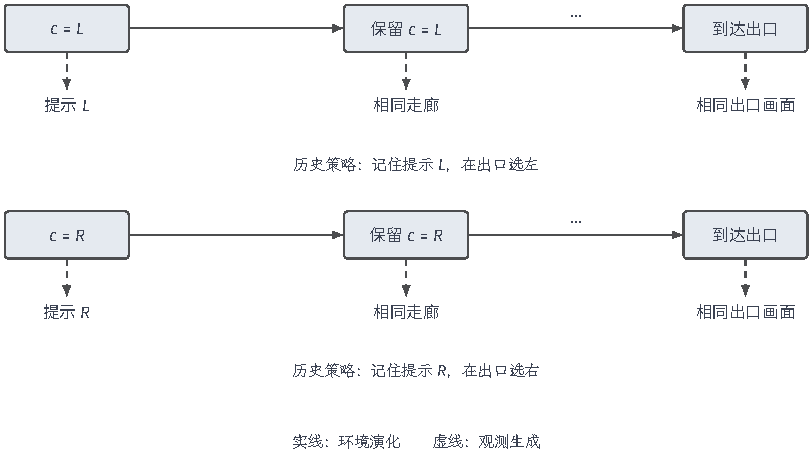
\includegraphics[width=137.534mm]{figures/10-reinforcement-learning/02-information-and-reward/tikz/rl-information-aliasing.pdf}
  \caption{早期提示任务中的两条可能轨迹。实线描述隐藏状态演化，虚线描述观测生成，途中固定为前进的动作未画出。出口画面相同，旁边单列的历史策略却因记住不同提示而选择相反方向；这些动作不属于观测。}
  \label{fig:rl-information-aliasing}
\end{figure*}

仿真器有时能在训练日志中给出$s_t$，帮助训练评论家或表示。但部署时若只能取得$o_t$，执行策略就不能读取这一特权状态，评价时也须提供部署真正可用的历史。要利用状态模型而不直接观测状态，可以推断当前状态的概率分布；下面的信念方法正是通过这一分布连接推断与决策，经典POMDP论述也采用这一思路\scite{rl1-kaelbling1998-pomdp}

% Outline: 4.2.2
\subsection{将可得历史压缩为决策状态}
\label{sec:rl-information-sufficiency}

完整历史保留了已记录的线索，但记录长度会随时间增长。下一次动作通常不需要逐字重读每个旧画面，只需要旧线索对当前状态判断留下的影响。模型已知时，可以为每个可能状态保存一个概率：过去动作先改变状态预测，新观测再改变各状态的相对可能性。这份分布称为信念状态（belief state），表示依据目前证据对真实状态的判断；它既压缩历史，又保留尚未排除的可能性。

如果把“障碍在左侧的概率为0.6”直接改成“障碍在左侧”，右侧仍有0.4概率这一可能性就被删掉了。碰撞成本很高时，这部分概率可能改变应选的动作。要说明保留完整分布为何足以支持控制，需要证明：预测奖励、更新状态推断和比较动作，都可以只使用信念完成。

\begin{definition}[信念状态]
  \label{def:rl-information-belief}
  给定有限POMDP，其隐藏状态集为$S$，策略按行动前可得的观测、过去动作与可见奖励历史$I_t$选择动作。对该过程生成律下具有正概率的可达历史$I_t$，\term{信念状态}（belief state）为
  \[
    b_t(s)=\mathbb P(s_t=s\mid I_t),\qquad
    b_t\in\Delta(S),
  \]
  其中$\Delta(S)$是$S$上的概率单纯形，即所有状态概率非负且总和为1的分布集合。$b_t$是给定历史后的后验分布，不表示另一个物理状态；只留下$\argmax_s b_t(s)$得到的点估计也不等于信念。
\end{definition}

推断从回合开始便已发生。对于具有正概率的初始观测$o_0$，按初始分布与观测似然加权并归一化，得到
$b_0(s)=\mu_0(s)K_{o,0}(o_0\mid s)/\sum_{\bar s}\mu_0(\bar s)K_{o,0}(o_0\mid\bar s)$；
仅当初始观测不改变关于初态的分布判断时，$b_0$才可直接取为$\mu_0$。

可以用带噪提示的教学变体核算初始更新。真实左右提示先验各为$1/2$，传感器以$0.8$概率报告正确提示。收到“左”时，“真实左且报告左”的概率为$0.5\times0.8=0.4$，“真实右却报告左”的概率为$0.5\times0.2=0.1$。报告左的总概率为$0.5$，归一化后真实左、右的概率为$0.8,0.2$。新观测增强了左的证据，却没有证明右不可能；再收到其他反馈时，还要继续更新这两个概率。

要证明压缩后没有丢掉最优决策所需的后果预测依据，不能只看这一次推断正确。还需检查三个操作是否都能从当前信念完成：预测一个动作带来的奖励和反馈，收到反馈后生成下一信念，按这些预测比较后续行为。下面的证明依次完成这三步，再用有限时域的反向归纳说明最优策略确实可以只读信念和时刻。

\begin{theorem}[精确信念对最优控制充分]
  \label{thm:rl-information-belief-sufficient}
  考虑定义~\ref{def:rl-information-pomdp}~中的已知有限POMDP，并假设动作选择仅依赖完整记录历史与独立的策略随机数。每个时刻$t$的最优历史价值都能写成$V_t^*(I_t)=U_t^*(b_t)$，且存在仅以$(t,b_t)$为依据的最优策略。
\end{theorem}

\begin{proof}
  先检查信念能否预测一个动作的后果。固定正概率历史$I_t$并选择$a$；由于动作只依据该历史和独立随机数，给定历史后的动作本身不再透露隐藏状态。按当前各状态的概率加权联合核，全概率公式给出
  \[
    \mathbb P(s_{t+1}=s',y_{t+1}=y\mid I_t,a)
    =\sum_s b_t(s)K(s',y\mid s,a).
  \]
  为预测可见反馈，将上式对隐藏的下一状态$s'$求和，得到
  $q(y\mid b_t,a)=\sum_{s,s'}b_t(s)K(s',y\mid s,a)$；将奖励取期望，得到
  $\bar R(b_t,a)=\sum_s b_t(s)R(s,a)$。反馈概率和奖励期望都由$(b_t,a)$确定。

  反馈出现后还需要更新推断。对$q(y\mid b_t,a)>0$的反馈，以其概率归一化状态与反馈的联合概率，贝叶斯公式给出
  \[
    b_{t+1}(s')
    =\frac{\sum_s b_t(s)K(s',y\mid s,a)}
           {q(y\mid b_t,a)}
    =:\tau(b_t,a,y)(s').
  \]
  新信念只需旧信念、动作和新反馈便可算出，这就是后验递推闭合；已经压缩的其余历史无需再读。零概率反馈不贡献期望，因此任意指定这些反馈上的$\tau$都不改变价值。

  最后用反向归纳检查最优动作比较。终点满足$V_H^*(I_H)=0$，可令$U_H^*(b)=0$。假设$t+1$时已有$V_{t+1}^*(I)=U_{t+1}^*(b(I))$；那么在$t$时选择$a$，当前奖励加上按可能反馈加权的最优继续价值为
  \[
    \bar R(b_t,a)
    +\gamma\sum_y q(y\mid b_t,a)
                      U_{t+1}^*(\tau(b_t,a,y)).
  \]
  上式仅依赖$b_t$与$a$。动作都来自有限动作集，按期望回报从中取最大值，便定义了$U_t^*(b_t)$并完成这一步归纳。在每个$(t,b)$处选取最大化动作，以固定规则处理平局，就构造出达到该值的信念策略。归纳到$t=0$，结论成立。
\end{proof}

这一结果说明最优控制不必保留信念以外的历史，并没有要求所有历史策略都在相同信念下选择同一动作。控制器可以故意按一个与未来无关的旧观测切换动作；这只是它使用了额外历史，不影响最优信念策略的存在。

上述构造需要已知模型；模型未知时，精确后验也不能直接计算。学习型潜在信念尝试用$\bm z_t$编码隐藏状态的不确定性。

信念记录的是隐藏状态概率；也可以换一个记录对象，直接保存“现在执行某串动作，会看到某串反馈”的概率。如果这些预测足以推算其他所需试验，就能直接比较动作后果，不必先恢复一套有语义名称的隐藏状态。指定动作是试验的条件，不是随机结果的一部分，这一区别会影响日志中应计算哪种概率。

另一种选择是\term{预测状态表示}（predictive state representation, PSR），用若干未来试验发生的预测概率概括历史。“试验”包含指定的未来动作和随后要观察的反馈，因此只预测收集策略自然产生的下一帧还不够。计算试验概率时，应按协议执行指定动作，再对环境反馈求概率，不能把行为策略恰好选择这些动作的概率乘进去。用日志条件频率估计试验概率时，还须说明所条件化的历史与采集随机化；仅筛出未来动作恰好匹配的记录，一般不足以完成这种校正。若这些概率能够递推所有相关试验，就可不必为隐藏状态赋予语义名称；表示是否有限维、能否从指定采集协议下的历史、动作和反馈记录学习，仍依赖结构条件\scite{rl4-littman2001-psr}

\begin{example}[动作试验概率与一次预测更新]
  \label{ex:rl-information-psr-test}
  令隐藏量$U\in\{0,1\}$在回合内保持不变，奖励均为0。执行动作$A$后观测为$U$，执行$B$后观测为$1-U$。可用“执行$A$后看到1”的概率$\zeta_t$概括当前历史；若$\zeta_t=0.3$，则“执行$B$后看到1”的概率为$0.7$。执行$A$并实际看到1后，更新为$\zeta_{t+1}=1$，随后执行$B$看到1的概率便为0。这个更新只需旧预测、执行动作和新观测。

  若采集者独立地以$0.2$概率选择$A$，日志中“选择$A$且看到1”的联合概率为$0.2\times0.3=0.06$；它包含采集动作的概率，不是执行$A$这一试验时看到1的概率$0.3$。
\end{example}

选择学习目标时，还要明确表示对什么问题充分。表~\ref{tab:rl-information-sufficiency}~分别考察未来反馈、固定策略价值和最优控制。例如，在两个隐藏状态中，“始终停止”的价值均为0，但向左、向右的奖励恰好相反。常数表示能准确预测停止策略的价值，却无法帮助选择转向动作。固定策略价值充分，不能据此推出改进所需的充分性。

\begin{table*}[htbp]
  \centering
  \small
  \begin{tabularx}{\linewidth}{p{25mm}XXX}
    \toprule
    充分性要求 & 必须保留的量 & 动作或策略范围 & 仍可丢失什么 \\
    \midrule
    未来反馈预测充分 & 各允许动作试验下的未来反馈联合分布与可递推状态 & 声明的全部试验，通常跨多个动作与时域 & 对这些预测无影响的历史细节与隐藏状态名称 \\
    给定策略价值充分 & 给定$\pi$和奖励下的条件期望回报 & 只要求该$\pi$的继续行为；还需说明执行时可读取的观测与历史 & 其他动作的价值、完整反馈分布 \\
    最优控制充分 & 允许策略类中达到最优值所需的动作比较与更新 & 所允许的控制行为；依赖任务与时域 & 不影响最优动作的预测细节 \\
    \bottomrule
  \end{tabularx}
  \caption{三种充分性对应不同问题。固定策略的回报预测正确，仍可能缺少评价其他动作或另一奖励函数所需的历史差别；已知POMDP中的精确信念则具有最优控制充分性的依据。}
  \label{tab:rl-information-sufficiency}
\end{table*}

% Outline: 4.2.3
\subsection{新观测到来后的决策状态更新}
\label{sec:rl-information-filtering}

信念充分性证明中，每次取得反馈都要生成新信念。实际计算时，给定已执行的$a_t$和收到的$y_{t+1}=(r_t,o_{t+1})$，先遍历可能的前态，用旧信念加权联合核，得到
$\widetilde b_{t+1}(s')=\sum_s b_t(s)K(s',y_{t+1}\mid s,a_t)$。这是下一状态与该反馈同时出现的概率，尚未归一化。再对所有下一状态求和，算出模型赋予该反馈的总概率；以它为分母，得到给定反馈后的状态分布：
\begin{equation}
  \label{eq:rl-information-bayes}
  b_{t+1}(s')
  =\frac{\sum_s b_t(s)K(s',y_{t+1}\mid s,a_t)}
         {\sum_{\bar s}\sum_s b_t(s)K(\bar s,y_{t+1}\mid s,a_t)}.
\end{equation}
这个条件分布只在分母为正时有定义。真实反馈若在模型中概率为0，滤波器便无法按上式归一化，需要检查模型或传感假设是否与实际过程失配。

若希望先预测状态、再单独用观测校正，就需要对联合核增加条件。假设
$K(s',(r,o')\mid s,a)=T(s'\mid s,a)K_o(o'\mid s',a)p(r\mid o',a)$，
这表示给定$o'$与$a$后，奖励不再改变对前后状态的条件分布判断。此时奖励项在分子分母中相同，可以约去；先对前态加权转移核，再按新观测的似然重新加权和归一化，得到
\begin{align}
  \label{eq:rl-information-predict-correct}
  b_{t+1}^{-}(s')&=\sum_sT(s'\mid s,a_t)b_t(s),\\
  b_{t+1}(s')&=
  \frac{K_o(o_{t+1}\mid s',a_t)b_{t+1}^{-}(s')}
       {\sum_{\bar s}K_o(o_{t+1}\mid\bar s,a_t)b_{t+1}^{-}(\bar s)}.
  \nonumber
\end{align}
碰撞奖励若由隐藏状态决定且提供了观测以外的线索，这一分解条件便不成立，更新时仍须保留奖励。

预测—校正也可以用于连续位置。此时不能逐个列出所有实数状态；若后验为高斯分布，就用均值$m_t$记录中心，用方差$\Sigma_t$记录不确定性。执行已知位移后，预测中心跟着移动；过程噪声增大预测方差。传感器再提供另一份带噪测量，校正应综合预测与测量的精度，而非总相信较新的那个数。

\begin{example}[一次标量滤波]
  \label{ex:rl-information-kalman}
  用标量教学系统$x_{t+1}=x_t+u_t+w_t$、$o_{t+1}=x_{t+1}+v_{t+1}$核算一次更新。给定已取得的历史，设当前状态的后验为$\mathcal N(m_t,\Sigma_t)$。过程噪声$w_t$与观测噪声$v_{t+1}$相互独立，也独立于当前状态和已取得的历史，均为零均值高斯量，方差分别记为$W,N$；另行记录的奖励不提供观测以外的状态线索。当前$m_t=0$、$\Sigma_t=1$，令已知控制量$u_t=1$、$W=N=1$，随后观测到2。状态预测为$m^-_{t+1}=1$、$\Sigma^-_{t+1}=2$，由此算得增益$2/3$。观测比预测大1，校正得到$m_{t+1}=1+(2/3)(2-1)=5/3$、$\Sigma_{t+1}=2/3$。方差尚未归零，所以$5/3$是后验均值，不是已知的真实位置。
\end{example}

这次增益$2/3$并非任意平均。预测位置方差为2，测量噪声方差为1，测量更精确，所以校正把两者之差的$2/3$加到预测上。若测量噪声方差改为100，其他条件相同，增益变为$2/(2+100)=1/51$，相同的测量偏差只会带来很小修正。下面的卡尔曼公式推广这种按误差协方差决定权重的关系，并明确它在哪些模型条件下是精确后验。

有限状态可以直接更新每个状态的概率；连续状态则需要适合其分布结构的表示。线性高斯模型在下述条件下使后验保持高斯，只需存储均值和协方差。设
$\bm x_{t+1}=\bm A\bm x_t+\bm B\bm u_t+\bm w_t$，
$\bm o_{t+1}=\bm C\bm x_{t+1}+\bm v_{t+1}$；
状态、控制输入与观测分别属于$\mathbb R^{d_x}$、$\mathbb R^{d_u}$和$\mathbb R^{d_o}$。
$\bm A\in\mathbb R^{d_x\times d_x}$传播状态，$\bm B\in\mathbb R^{d_x\times d_u}$将控制输入映到状态变化，$\bm C\in\mathbb R^{d_o\times d_x}$将状态映到观测。初始状态为高斯；所有时刻的过程噪声$\bm w_t$、观测噪声$\bm v_{t+1}$与初始状态相互独立，两类噪声均为零均值高斯量，协方差分别为$\bm W\in\mathbb R^{d_x\times d_x}$和$\bm N\in\mathbb R^{d_o\times d_o}$。控制输入$\bm u_t$只依据行动前已得历史和与环境独立的策略随机数，因此当前过程噪声与新观测噪声不含历史相关项；另行记录的奖励暂不改变只依据观测形成的状态后验。当前后验为
$\mathcal N(\bm m_t,\bm\Sigma_t)$时，\term{卡尔曼滤波}（Kalman filter）先传播均值和协方差，再用实际观测与预测观测的差修正它们。预测与校正递推为
\begin{align}
  \label{eq:rl-information-kalman}
  \bm m^-_{t+1}&=\bm A\bm m_t+\bm B\bm u_t,&
  \bm\Sigma^-_{t+1}&=\bm A\bm\Sigma_t\bm A^\top+\bm W,\nonumber\\
  \bm L_{t+1}&=\bm\Sigma^-_{t+1}\bm C^\top
     (\bm C\bm\Sigma^-_{t+1}\bm C^\top+\bm N)^{-1},\nonumber\\
  \bm m_{t+1}&=\bm m^-_{t+1}
       +\bm L_{t+1}(\bm o_{t+1}-\bm C\bm m^-_{t+1}),\nonumber\\
  \bm\Sigma_{t+1}&=(\bm I-\bm L_{t+1}\bm C)\bm\Sigma^-_{t+1}.
\end{align}
式中$\bm I$为$d_x$维单位矩阵，增益$\bm L_{t+1}$为$d_x\times d_o$矩阵，将观测差映为状态修正。创新$\bm e_{t+1}=\bm o_{t+1}-\bm C\bm m^-_{t+1}$就是实际观测相对预测观测的差；给定已有历史和当前控制输入，其协方差为
$\bm S_{t+1}=\bm C\bm\Sigma^-_{t+1}\bm C^\top+\bm N$，
状态预测误差与创新的交叉协方差为$\bm\Sigma^-_{t+1}\bm C^\top$。
在线性校正中，最小均方误差要求校正后的误差与创新正交，因而增益满足正规关系
$\bm L_{t+1}\bm S_{t+1}=\bm\Sigma^-_{t+1}\bm C^\top$。
这里要求$\bm S_{t+1}$可逆；解该关系便得到式中的增益，而不是任意选取预测均值与新观测的权重。联合高斯条件使这一线性校正等于条件均值；跨时独立条件保证预测式没有遗漏噪声与历史的交叉项。二者共同支持上述精确递推\scite{rl4-kalman1960-filter}。递推把传感历史压缩为下一次动作选择可用的状态后验；均值与协方差的闭合依赖这些线性高斯和独立性条件，并不适用于任意分布。相关状态估计结论可参考\BookChapterRef{chap:dynamical-systems-and-state-estimation}{卷2《数学准备：概率、因果与决策》中讨论动力系统的章节}。

这里的“创新”只表示测量与模型预测之间的新差额。预测和测量都可能出错，增益依据状态预测误差与这份差额的交叉协方差，以及差额自身的协方差设定，再把差额映成状态修正。联合高斯使条件均值可以由这种线性校正精确算出；若后验有两个相距很远的峰，仅保留均值和协方差就可能丢掉决定动作的重要区别，不能直接沿用同一个精确性结论。

显式模型若不可信，就不能直接依靠上述精确滤波。可以改为从按回合排列的交互训练记录学习递推记忆
$\bm z_{t+1}=f_{\bm\theta}(\bm z_t,a_t,r_t,o_{t+1})$，
也可以保留历史，再由注意力网络重新计算$\bm z_t$。图~\ref{fig:rl-information-memory}~对照了两种计算方式。用于计算记忆的观测、动作和奖励序列必须保持同一轨迹的时间关系，记忆按协议在回合开始重置；任意训练片段的开头未必是回合开始，不能在那里直接清零。

\begin{figure*}[htbp]
  \centering
  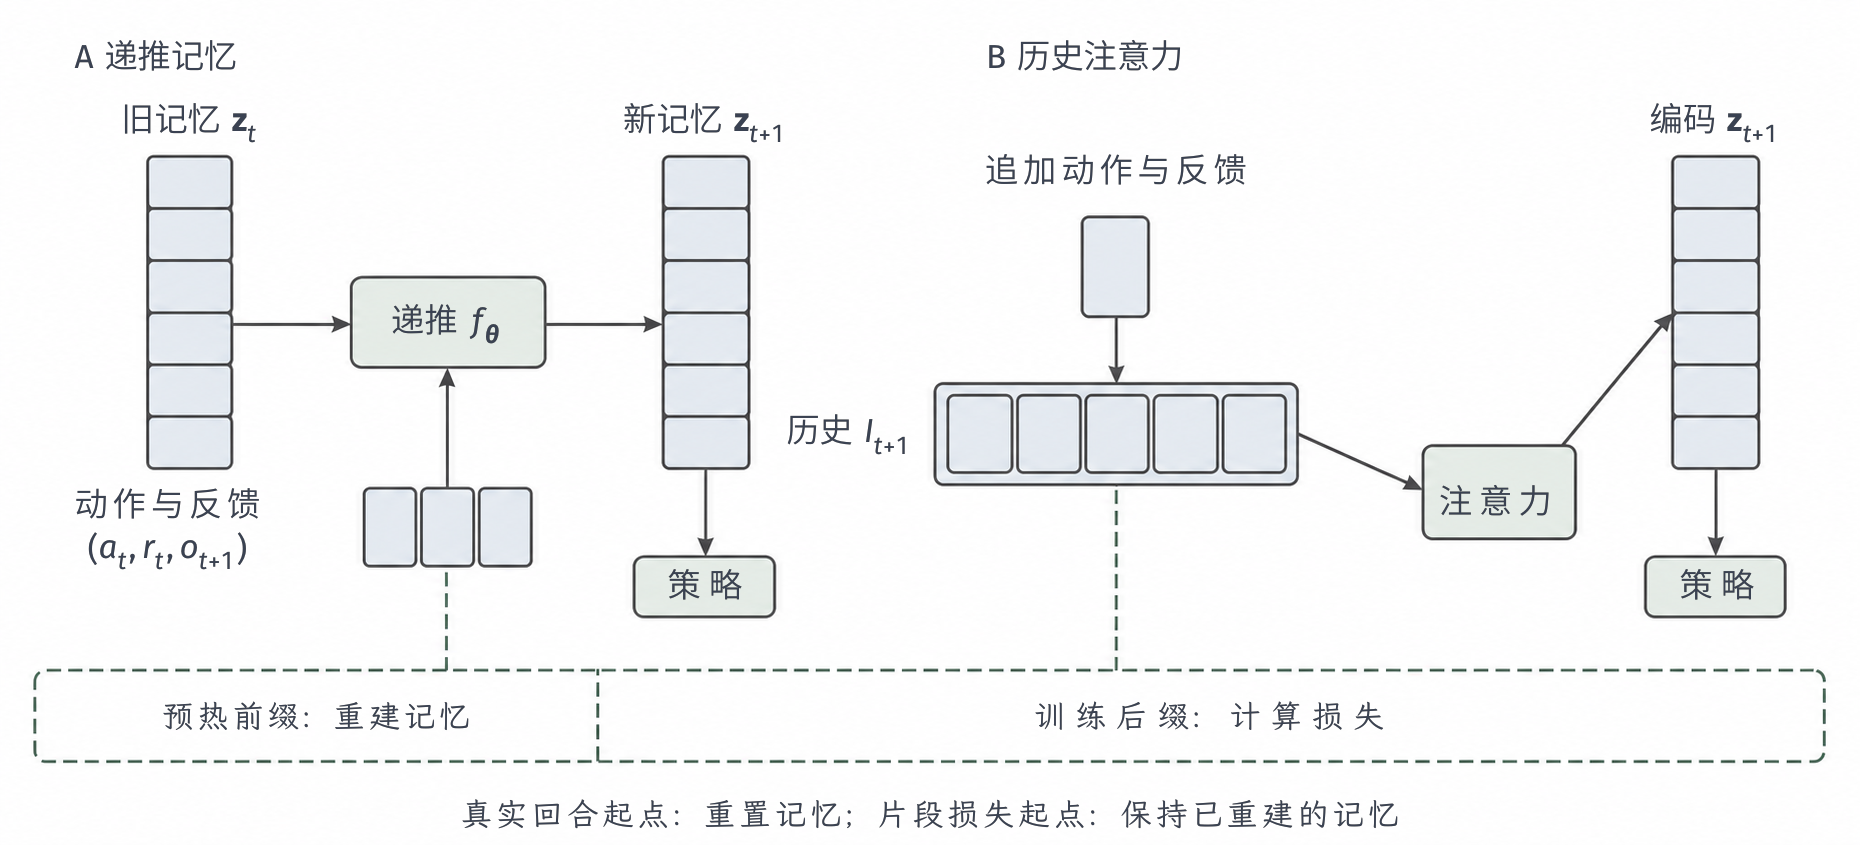
\includegraphics[width=157.400mm]{figures/10-reinforcement-learning/02-information-and-reward/generated/rl-information-memory/figure.png}
  \caption{递推记忆与历史注意力所用的交互记录及表示更新。实线描述表示与策略的计算，虚线标出训练片段及边界。预热前缀用于恢复损失起点处的记忆，不计算其训练损失。图示片段从真实回合开始；回合中部片段需用已保存状态或更早前缀初始化，片段边界本身不构成重置依据。向量与历史格数仅为示意，不规定状态维数或可见历史长度。}
  \label{fig:rl-information-memory}
\end{figure*}

训练片段与真实回合有不同边界。沿用早期提示任务，若片段从走廊中部开始，正确记忆应仍含入口提示；直接清零就使训练网络看到一段已经删掉提示的历史片段。预热让网络先读不计损失的前缀，恢复损失起点处的记忆；梯度截断则限制本次训练向多早传播。它们分别处理记忆的初始化与计算长度，不能用“只反传最近若干步”推断更早线索不重要。

\term{深度循环Q网络}（Deep Recurrent Q-Network, DRQN）将循环状态加入价值网络，使过去帧的特征可以影响当前估值。相对于堆叠有限帧，它改变了历史的保存方式，价值目标仍采用时序差分学习\scite{rl4-hausknecht2015-drqn}
序列进入重放后，还要处理参数变化导致的表示漂移和旧隐藏状态。\term{R2D2}（Recurrent Replay Distributed DQN）结合循环网络、序列重放与分布式训练，分析了这些问题。截断反向传播只限制梯度跨越多少步，并未说明更早的历史无用。burn-in即预热，先运行片段前缀恢复隐藏状态，再在后缀计算损失。也可以保存收集时的隐藏状态，减少从零启动的偏差；但网络参数更新后，保存的状态可能已不适合当前网络\scite{rl4-kapturowski2019-r2d2}

循环记忆每收到一个新记录，就把旧记忆与新取得的动作、奖励和观测变成下一记忆向量；被丢掉的细节以后通常无法重新读取。历史注意力则保留一批过去编码，计算当前表示时可以重新按相关性加权读取。前者用固定维数递推，后者用随保留窗口增长的缓存换取重读机会。两种结构都需要学习保留哪些线索，结构本身不等于已经得到精确信念。

注意力模型也可以跨片段保留过去观测、动作和奖励的编码。\term{GTrXL}（Gated Transformer-XL）在Transformer-XL中引入门控等结构调整，以适配强化学习优化。外部记忆则将历史写入独立存储，再按需读取。增加这些保存能力会带来缓存、读写和训练成本。更长的上下文或更低的预测损失，只描述保留的历史范围或训练记录上的拟合结果，尚不能证明表示满足定理~\ref{thm:rl-information-belief-sufficient}~的条件。

% Outline: 4.2.4
\subsection{基于决策状态的策略求解与动作选择}
\label{sec:rl-information-belief-control}

信念更新给出当前各状态的概率，我们还需要据此决定动作。比较时要平均可能状态的后果，并允许后续动作随新反馈改变，不能先挑一个最可能状态当成真相。\term{信念MDP}（belief MDP）把可计算的信念本身作为完全可见的决策状态。其即时奖励为
$\bar R(b,a)=\sum_s b(s)R(s,a)$，反馈概率为
$q(y\mid b,a)=\sum_{s,s'}b(s)K(s',y\mid s,a)$，状态转移通过$\tau(b,a,y)$实现。
要计算剩余时域的最优回报，可以对有限动作集$\mathsf A$中的每个动作，加上即时奖励和按反馈概率加权的继续价值，再选最大的期望回报。第~\ref{chap:rl-planning}~章的Bellman关系由此写成
\begin{equation}
  \label{eq:rl-information-belief-bellman}
  U_t^*(b)=\max_a\left\{
    \bar R(b,a)+\gamma\sum_yq(y\mid b,a)
                    U_{t+1}^*(\tau(b,a,y))\right\},
  \qquad U_H^*=0.
\end{equation}
反馈不可由控制器挑选，必须逐个更新信念、计算继续价值后按发生概率取期望。一般不能用
$U_{t+1}^*(\mathbb E[b_{t+1}])$替代$\mathbb E[U_{t+1}^*(b_{t+1})]$，因为后续动作依据实际反馈而非平均反馈选择；先平均信念会丢掉这种适应机会。

\begin{example}[Tiger中的倾听、更新与开门]
  \label{ex:rl-information-tiger}
  Tiger任务有两扇门，一侧藏着危险，另一侧可以获得奖励。隐藏状态$s\in\{L,R\}$表示危险的方向。打开安全门得10，打开危险门得$-100$，随后回合终止；倾听得$-1$，状态不变，以0.95的概率报告正确方向。令初始$b_0(L)=b_0(R)=1/2$，最多行动两次，$\gamma=0.9$，时域结束后价值为0。这些数值与两步终止规则仅用于教学，不代表所有Tiger版本。

  先比较不额外倾听的开门动作。直接打开任意一扇门，按初始危险概率加权，期望奖励都是
  $(1/2)10+(1/2)(-100)=-45$。若先倾听并得到“左侧有声”，用正确报告和错误报告的概率更新左侧危险概率，得到
  \[
    b_1(L)=\frac{0.95(1/2)}
                        {0.95(1/2)+0.05(1/2)}=0.95.
  \]
  按更新后的信念，开右门的期望奖励为$0.95(10)+0.05(-100)=4.5$，
  开左门为$0.95(-100)+0.05(10)=-94.5$；
  再次倾听只能得$-1$，之后已无动作可用，因此在这三个动作中应开右门。
  若听见右侧，按对称计算应开左门。两种反馈各以$1/2$发生，将各自的最优开门价值加权、折扣，再扣除倾听成本，初始倾听价值为
  \[
    Q_0(b_0,\text{倾听})
       =-1+0.9\bigl[(1/2)4.5+(1/2)4.5\bigr]=3.05.
  \]
  在此两步设定下，先倾听再按反馈开门的期望回报为3.05，高于直接开门的$-45$。
\end{example}

图~\ref{fig:rl-information-tiger}~显示了按反馈分开的动作比较。若固定同一个开门时刻，并把信号设为免费，最优开门收益的期望增量为$4.5-(-45)=49.5$；实际两步方案还包含倾听成本与后续折扣，不能直接使用这个增量。模型和听觉准确率虽然已知，当前危险位置仍未知，所以倾听可能有用。剩余时间不足、先验已很确定或探测成本过高时，倾听带来的开门收益增量可能不足以支付探测代价，直接开门反而更合适。

\begin{figure*}[htbp]
  \centering
  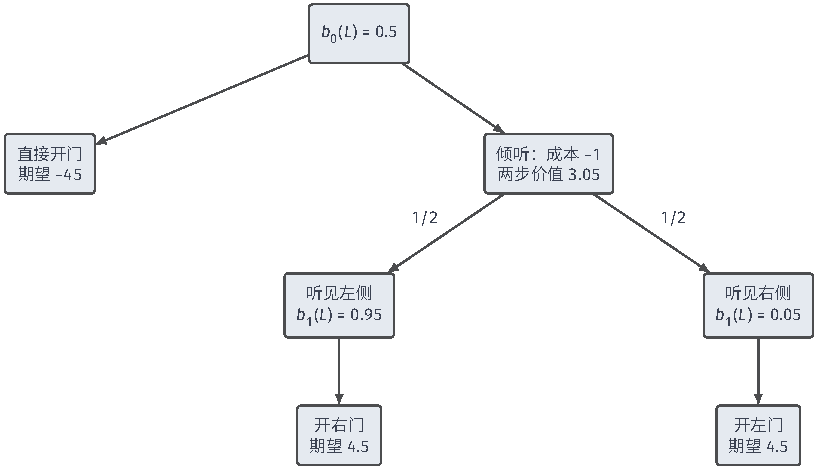
\includegraphics[width=138.511mm]{figures/10-reinforcement-learning/02-information-and-reward/tikz/rl-information-tiger.pdf}
  \caption{教学Tiger的两步决策树。$b(L)$是左门后有危险的概率。倾听反馈各以$1/2$发生，随后按新信念选择安全概率较高的门。末端标注条件期望开门奖励，根节点的3.05则计入倾听成本和折扣。}
  \label{fig:rl-information-tiger}
\end{figure*}

若只保留先验概率最大的状态，平局时任取一侧为危险，再照完全可观测解打开另一侧，预测奖励会是10，真实期望却是$-45$。这不只是平局处理的问题。将先验改为$b_0(L)=0.6$，点估计仍直接开右门，但真实期望为$0.6(10)+0.4(-100)=-34$；按0.95准确率计算两个倾听分支，先听再开的价值仍是3.05。被删除的另一侧概率影响了是否值得付费倾听，也就影响了当前动作。

\begin{example}[Tiger最后一步的回报向量]
  \label{ex:rl-information-alpha-vectors}
  沿用例~\ref{ex:rl-information-tiger}的奖励，在只剩一次行动时，按隐藏状态$(L,R)$排列，开左门、开右门和倾听对应的向量分别是$(-100,10)$、$(10,-100)$和$(-1,-1)$。令$p=b(L)$，三个信念价值分别为$10-110p$、$110p-100$和$-1$，所以$U_1^*(b)$是三者的最大值。$p=0.5$时选择倾听，价值为$-1$；$p=0.95$时选择开右门，价值为$4.5$。若只保留在$p=0.5$最优的向量，就会把$p=0.95$处的价值也估成$-1$。同一组向量在不同信念下有不同的最优者。
\end{example}

最后一步中，每个动作在两个隐藏状态下的回报构成一个向量，信念只负责给它加权。现在将这一计算推广到多步条件计划：后续动作可以随反馈分支改变，但仍能分别计算整份计划从各隐藏状态出发的期望回报。要在所有信念上比较计划，可以先保存这些回报向量，再据当前信念计算每份计划的价值。在有限非空状态集$S$、动作集$\mathsf A$、可见反馈集$\mathcal Y$及正整数时域$H$下，固定已知模型$K,R$、$0\leq\gamma\leq1$和零终端价值。把从$t$起的确定性策略写成深度至多$H-t$的条件树$\sigma$：节点规定动作，分支对应下一次可见反馈。分别从每个隐藏状态$s$开始执行这棵树，将期望折扣回报记为$\alpha_t^\sigma(s)$，这些数构成向量$\bm\alpha_t^\sigma\in\mathbb R^{|S|}$。在信念$b$下执行同一棵树的价值就是$\sum_s b(s)\alpha_t^\sigma(s)$；有限时域内这样的树只有有限棵，随机化也不能超过其中最优者。令$\bm\Lambda_t$收集这些回报向量，便有
\begin{equation}
  U_t^*(b)=\max_{\bm\alpha\in\bm\Lambda_t}\sum_{s\in S}b(s)\alpha(s).
  \label{eq:rl-information-alpha-envelope}
\end{equation}
因此，奖励最大化时的最优价值是信念单纯形上的分段线性凸函数：每棵树贡献一个线性函数，逐点取最高者形成上包络。这使连续信念上的价值比较转成有限向量比较，相关凸性背景可参考\BookChapterRef{chap:optimization}{卷1《数学准备：计算、分析与几何》中讨论最优化的章节}。

“分段线性”来自计划切换。仍令$p$为左侧危险概率，一个计划的价值是关于$p$的直线；在某个$p$范围内它最高，换到另一个范围时可能由另一条直线最高。最优值因此是这些直线的上包络，而不是把计划的回报向量先平均。一般信念有多个概率坐标，道理相同：计划固定时加权价值线性，优化时逐点选择不同计划。

完整备份须组合各反馈分支的后继树，向量数量会迅速增长。\term{点基值迭代}（point-based value iteration, PBVI）改在有限个代表信念上备份。在上述有限时域形式中，从终端零向量出发，对某个代表信念和候选动作，先在当前保留的后继向量中选出对各反馈后信念价值最高者，再把当前奖励与这些向量的模型加权折扣和合成为新向量，保留在该代表信念处价值最大的候选。这样保留下来的是定义在整个信念空间上的线性函数，而不只是各代表点的数值；但没有保留的向量仍可能在别处最优，代表信念的覆盖会影响近似质量\scite{rl4-pineau2003-pbvi}。

有限状态控制器（finite-state controller）则把过去的观测、动作和奖励压成有限个记忆节点，每个节点规定动作分布，收到反馈后按规则跳到下一节点。例如，两个节点可以分别记住左右提示，选择出口时读取节点即可。节点数限制控制器能区分多少种记忆情况，直接限制可实现的历史策略。两者分别近似价值函数和策略记忆，不能混作同一种压缩。

在特定控制问题中，估计与控制确实可以分开。线性、高斯、模型已知且没有额外约束的二次成本控制满足相应条件时，\term{线性二次高斯控制}（linear-quadratic-Gaussian control, LQG）的分离原则允许把Kalman估计的状态均值交给线性最优反馈控制器。噪声和观测机制还须与动作无关；无限时域稳定解另需可稳定性、可检测性等条件。动作若能改变观测质量，或额外奖励改变了关于隐藏状态的后验，就不能直接沿用该结论。Tiger中的倾听恰好改变后续收到的观测，因此一般POMDP没有先独立估计、再按已知状态控制的普遍保证。

模型未知时，可以把学习到的$\bm z_t$接入第~\ref{chap:rl-learning}~章的方法。循环价值学习用它构造自举目标，循环行动者—评论家用它计算动作分布和优势，潜在模型则在该表示上学习转移与奖励，用于规划或想象轨迹。这些方法学习表示、价值或动力学，但还须检查表示是否能判断未实际执行的其他动作会怎样，即是否保留了预测各候选动作后果所需的历史差别。

% Outline: 4.2.5
\subsection{近似决策状态的误差与计算边界}
\label{sec:rl-information-memory-errors}

选择历史表示时，除网络参数外，还要计算保存历史、更新表示和随后规划的成本。表~\ref{tab:rl-information-memory-cost}~按$n_S=|S|$、历史长度$t$、窗口长度$L$、单步记录的编码维度$d$、循环隐藏维度$m$和控制器节点数$n_C$列出直接实现的复杂度。这些是表中指定计算方式的成本，不是对全部模型的复杂度断言。

\begin{table*}[htbp]
  \centering
  \small
  \begin{tabularx}{\linewidth}{p{21mm}XXXX}
    \toprule
    表示 & 历史范围与存储 & 一次更新代价 & 决策或规划空间 & 充分性依据 \\
    \midrule
    完整历史 & 全部；$O(td)$ & 追加记录$O(d)$；重新读取至少随$t$增长 & 分支随时域增长的历史树 & 不主动丢弃已记录的观测、动作与奖励 \\
    精确信念 & 历史递推压缩；$O(n_S)$ & 稠密有限核$O(n_S^2)$ & $n_S-1$维单纯形；有限层可达点也可指数增长 & 已知正确模型下的充分性定理 \\
    有限窗口 & 最近$L$步；$O(Ld)$ & 缓冲追加$O(d)$，编码另计 & 窗口内记录；未必马尔可夫 & 需证明任务只依赖该窗口 \\
    有限状态控制器 & 当前节点$O(1)$；节点表另计 & 表查找可为$O(1)$ & $n_C$个记忆节点上的策略 & 策略类限制；一般非充分 \\
    学习型记忆 & 循环$O(m)$；注意力缓存随$L$增长 & 稠密循环$O(m^2+md)$；标准全窗口注意力$O(L^2m+Lm^2)$ & 学习表示上的价值或策略 & 任务与模型假设，加独立验证 \\
    \bottomrule
  \end{tabularx}
  \caption{历史与状态表示的成本及依据。注意力复杂度按宽度$m$的一层完整窗口计算，增量缓存可改变单步成本；有限状态控制器若按节点与反馈跳转，跳转表需$O(n_C^2|\mathcal Y|)$存储，若另依赖实际动作，还需乘$|\mathsf A|$。存在充分统计量不等于易于规划。}
  \label{tab:rl-information-memory-cost}
\end{table*}

例如，GTrXL中的门控与残差调整主要帮助训练保持稳定，注意力缓存和计算仍随实际保留的序列长度变化。能否较顺利地训练，与学到的表示能否充当精确决策状态，需要分别核查\scite{rl4-parisotto2020-gtrxl}

要理解压缩怎样影响动作，可以沿表示、初始化、模型和求解逐一追踪。两个历史若被编码为同一$\bm z$，却在同一动作下具有不同的反馈分布或价值，单凭$\bm z$就无法区分它们；增加训练轮数不能恢复这种表示遗漏。表示本来能保存提示，却在每个重放片段开始被清零，则是初始化错误。联合核估计不准和正确目标下优化尚未收敛，又是不同误差，各自需要对应的修正。

若要把这些误差转换为动作损失，就需要对动作价值的误差作出明确假设。固定历史$I$，在同一允许动作集上比较真实最优继续价值和近似值；假设各动作都有
$|\widehat Q(I,a)-Q^*(I,a)|\leq\delta$。分别按近似值和真实值选取最大化动作
$\hat a\in\argmax_a\widehat Q(I,a)$、$a^*\in\argmax_aQ^*(I,a)$；插入这两个动作的近似价值，真实损失满足
\[
  Q^*(I,a^*)-Q^*(I,\hat a)
  \leq
  [Q^*(I,a^*)-\widehat Q(I,a^*)]
  +[\widehat Q(I,\hat a)-Q^*(I,\hat a)]
  \leq2\delta.
\]
中间省去的差为非正，因为$\hat a$最大化近似值，即$\widehat Q(I,a^*)\leq\widehat Q(I,\hat a)$。这一界要求逐动作误差受控，平均重建损失没有直接提供该条件；没有表示误差到价值误差的论证，就不能把训练损失当作$\delta$。

例~\ref{ex:rl-information-cue}~还可以直接检验重建与控制的区别。沿用不折扣成功奖励，两个记忆节点分别保存左右提示即可达到期望值1，丢弃提示则至多达到$1/2$。即便窗口内每帧都完美重建，$1/2$的控制差距仍在。若奖励后来改为依赖另一条早期线索，仅保存$c$又可能不足，当前任务充分性不能扩展为对所有奖励目标充分。第~\ref{chap:rl-learning}~章讨论更一般的样本复杂度与函数类条件；本例先表明，表示删去的历史线索不能靠更多样本或更充分的优化补回。

% Outline: 4.3
\section{固定经验下的策略评价与选择}
\label{sec:rl-information-evaluation}

% Outline: 4.3.1
\subsection{固定经验与行为策略}
\label{sec:rl-information-logging}

下面暂时恢复完全可观测条件：每条记录都有完整状态，但学习者不能再到环境中试验。要用这些记录评价另一策略，先要弄清动作由谁、按什么概率选出。同一份状态动作表可能来自固定策略、多个策略的混合或持续更新的控制器；收集方式不同，概率校正和误差估计所用的条件也不同。

\begin{definition}[行为策略与目标策略]
  \label{def:rl-information-behavior}
  固定完全可观测环境、正整数时域$H$、$0\leq\gamma\leq1$及奖励绝对可积的回合。\term{行为策略}$\beta$生成日志动作，\term{目标策略}$\pi$是待评价或部署的决策规律。将收集的$n\geq1$个回合写为
  \[
    D=(Z_1,\ldots,Z_n),\qquad
    Z_i=(s_{i,0},a_{i,0},r_{i,0},\ldots,s_{i,H}).
  \]
  每条$Z_i$是一回合的可见记录，按采集顺序保留重复回合；状态完全可见，因而这些状态字段可以记录。理论轨迹律记为$P_{\mathcal E}^\beta$，实际记录律为$P_{\mathrm{rec}}^\beta$，两者由保留实际字段的记录映射联系。该记录组写法本身不假设各回合独立。
  有限时域评价采用价值
  $J_H(\pi)=\mathbb E_\pi[\sum_{t=0}^{H-1}\gamma^t r_t]$。
  若回合提前终止，则以吸收状态和零奖励补到$H$。$J_H$只累计有限时域，不等于无限时域的$J$；后文切换目标时将另作说明。
\end{definition}

这里有三种不同对象：环境规律规定执行动作后的真实结果，行为策略规定日志中动作怎样被选出，记录规则规定哪些字段被保存。$D$是这些机制某一次运行留下的有限材料，记录律则描述按同一协议反复采集时会出现怎样的材料。即使当前三条轨迹都相同，也不意味着其总体分布只允许这条轨迹；评价要分清样本中暂时没出现与收集机制从来不会产生。

下文$p_\sigma$表示可见记录律$P_{\mathrm{rec}}^\sigma$在离散情形的质量函数，或相对于固定共同支配测度的密度，其中$\sigma\in\{\beta,\pi\}$。支持条件针对相同记录字段；策略版本等采集元数据用于说明生成机制，不能未经说明就当成目标策略也必须复现的记录字段。

有限记录组$D$是训练或评价所用的实现样本，$P_{\mathrm{rec}}^\beta$描述这类记录的总体规律；两者都与环境及观测核所规定的生成机制不同。回合是否独立、怎样抽取转移及如何划分训练和评价记录，还须由采样协议说明。

单一马尔可夫行为策略可逐步记录$\beta(a_t\mid s_t)$。多个子策略混合时，必须区别抽取时机：每步重新按已知概率选择子策略，可以用该步混合权重加权动作概率；回合开始只抽一次，则历史会改变对所选子策略的后验，通常不能一直使用固定混合权重。后一种收集方式需要保存策略身份及相应概率并作适当的条件采样分析，或记录真正的$\beta_t(a_t\mid I_t)$；这里的历史包含行动前记录的完整状态、动作和奖励。身份字段说明了收集机制，却不能补齐某个条件层中缺失的目标动作。若策略随收集过程自适应更新，还须保存版本和选择机制。

\begin{example}[回合只抽一次控制器]
  \label{ex:rl-information-collector-mixture}
  设任务只有两步，状态只标记当前时刻。采集者在回合开始各以$1/2$概率选择“始终执行$A$”或“始终执行$B$”的控制器，于是只有$AA,BB$两种动作序列，各占$1/2$。看到首步$A$后，控制器身份已经确定，所以$\beta_1(A\mid I_1)=1$，不是$1/2$。

  对始终执行$A$的目标策略，$AA$的整轨概率比为$1/(1/2)=2$。若每步都误用固定混合概率$1/2$，就得到错误权重4。令首步奖励为0，第二步$A$得1、$B$得0，$\gamma=0.9$；正确的重加权期望为$(1/2)\times2\times0.9=0.9$，错误权重则给出1.8。回合混合与逐步混合不能只凭相同的起始权重互换。
\end{example}

动作概率描述采集者如何选动作，不是描述环境怎样给奖励。前面的回合混合例中，第一次动作揭示了本回合是哪一个控制器，所以第二次动作概率随已知历史改变；真实环境的奖励规律并未因此改变。评价必须使用实际发生的条件选择概率，才不会把同一条轨迹重复计权。

这些动作概率最好来自当时实际使用的随机化机制。机制记录正确时，概率是已知量；事后拟合的$\widehat\beta$则含有模型误差。确定性收集者没有尝试的动作，即使密度网络给出非零概率，也仍没有行为支持。表~\ref{tab:rl-information-fields}~说明哪些日志字段支撑评价中的具体计算。

\begin{table}[htbp]
  \centering
  \small
  \begin{tabularx}{\linewidth}{p{29mm}X}
    \toprule
    字段 & 支撑的计算与省略后的风险 \\
    \midrule
    状态、动作、奖励、下一状态 & 构造回报、Bellman目标及目标策略动作概率 \\
    真终止标记 & 真正终止后不再自举；终止奖励仍记在$r_t$ \\
    时间截断标记 & 区分任务结束与记录停止；持续任务截断处通常仍需继续价值 \\
    回合标识与时刻 & 恢复轨迹概率比、记忆重置和回合级划分 \\
    行为概率及策略版本 & 确定动作选择机制，区分已知概率与估计概率 \\
    初始条件、任务与目标 & 说明评价的$\mu_0$、奖励定义及任务分布是否匹配 \\
    \bottomrule
  \end{tabularx}
  \caption{完整状态日志仍需要采样元数据。有限时域的真正$H$步终止与持续任务在$H$处被时间截断，具有不同的自举目标。}
  \label{tab:rl-information-fields}
\end{table}

恢复回合边界后，还要确定统计重复的单位。独立收集的$n$个回合可以作为独立评价单位，回合内相邻转移却不能直接当作独立重复。只有一条相关长轨迹时，分块估计或相关记录的统计推断需要混合性等条件，即随时间间隔增加，相关性受到相应控制。若把相邻转移随机拆到训练与测试中，测试误差可能利用训练记录中已出现的同一条轨迹片段，也会高估独立样本数。

D4RL包含不同质量、收集者及混合任务的交互日志，因此报告时要保留具体版本、奖励定义和归一化分数的参照；仅称“专家混合日志”还不能确定实验所用的训练记录及其采集条件\scite{rl4-fu2020-d4rl}
除了日志记录组成，RL Unplugged还区分任务域与选模协议。调参是否使用在线策略测试尤其需要声明：如果依据真实环境分数选择超参数，整个选模过程就已超出纯固定经验评价\scite{rl4-gulcehre2020-unplugged}

Minari按回合提供回合记录及采集元数据接口，但具体数据集的终止、截断、环境版本和收集者说明仍须核对，存储格式并不保证行为概率可得\scite{rl4-farama-minari}
对于OGBench这样的离线目标条件强化学习基准，还要报告未记录奖励的交互轨迹组成、目标怎样选择、奖励怎样重标记以及测试目标协议。目标条件改变后，成功率不能直接横比。OGBench已有ICLR 2025正式版本；这里用它说明协议需包含哪些内容，不据其分数判断方法普遍优劣\scite{rl4-park2025-ogbench}

% Outline: 4.3.2
\subsection{策略价值的可识别性与覆盖条件}
\label{sec:rl-information-coverage}

固定日志可以交给多个候选策略评价，但每个候选会使用不同的状态动作。比较分数之前，先假设能够无限重复原收集方式，检查是否仍会有不同环境给出同样日志、却赋予候选不同价值。这是\term{可识别性}（identifiability）问题：可见回合记录的总体分布能否唯一确定目标量。若不能，增加同类样本也无法只靠估计精度解决。

\begin{definition}[策略价值可识别]
  \label{def:rl-information-identifiability}
  策略价值可识别性以给定的记录生成协议、可观察字段、环境结构假设、初始分布和目标策略为条件。若所有产生相同可见回合记录总体分布的允许环境都给出相同目标策略价值，则该价值可识别。这是总体分布的性质，不说明有限样本估计已经准确。
\end{definition}

\begin{theorem}[固定经验不能识别未覆盖动作的价值]
  \label{thm:rl-information-unseen-action}
  对单状态、单步、两个动作的任务，若日志行为只执行其中一个动作，且没有将两动作奖励联系起来的结构假设，则另一动作的价值及其相对行为策略的优劣一般不可识别。
\end{theorem}

\begin{proof}
  用两个仅在未见动作上不同的环境检验定义。唯一非终止状态为$s$，执行$a_0$或$a_1$后均终止。在$M_+$与$M_-$中，$a_0$的奖励都为0，$a_1$的奖励分别为$+1$和$-1$；两环境的行为均为$\beta(a_0\mid s)=1$。

  无论日志多大，其中只有$(s,a_0,0,s_{\mathrm{term}})$，所以可观测分布完全相同。但目标$\pi(a_1\mid s)=1$的价值分别是$+1$和$-1$，行为基线价值均为0。只使用日志的程序收到相同的有限日志记录组，在相同算法随机化规律下得到的估计或策略分布也相同，无法在两个环境中都正确确定目标价值或排序。因此，按定义，这两项结论都不可识别。
\end{proof}

这个反例中的障碍不是样本太少，而是收集规则永远不查$a_1$。如果不断重复同一规则，仍会得到完全相同的零奖励记录；在两个环境中，程序接收的证据始终一样。可识别性先检查这种“总体规律也不能区分”的缺口。只有通过这个检查，增加样本以提高估计精度才可能解决剩余困难。

给$a_1$产生数值预测还不够。神经网络可以外推，结构化动力学也可以用$a_0$的转移记录推断$a_1$的后果，但需要可核验的正确性假设说明两动作怎样联系，才可能排除上述一个环境。网络能表达这种联系，不表示日志已经证明它成立。

为检查哪些候选避开了这一缺口，可以比较候选诱导的轨迹分布和行为分布。候选可能使用而行为绝不产生的轨迹，无法通过日志重加权补出；即使没有这种绝对缺口，也要考察候选是否把大量概率放在日志极少涉及的区域。

\begin{definition}[支持、集中程度与部分覆盖]
  \label{def:rl-information-support}
  在相同可见记录空间上，目标支持条件为$P_{\mathrm{rec}}^\pi\ll P_{\mathrm{rec}}^\beta$：行为记录律赋予零概率的事件，目标记录律也赋予零概率。在共同环境核的有限模型中，目标可达历史上的每个目标动作都须有行为支持。

  若将评价改为无限时域折扣占用而非有限整条轨迹，则用前文归一化的$d^\pi(s,a)$表示目标访问概率，以$\nu(s,a)$表示训练转移记录的归一化采样分布。集中程度系数衡量目标访问相对训练记录采样可能集中到多大程度，用本质上确界记录占用比的上界而非平均大小，即取遍$\nu$支持中的状态动作、忽略$\nu$零测集。其定义为
  \[
    C_\pi=\operatorname*{ess\,sup}_{(s,a)\sim\nu}
               \frac{d^\pi(s,a)}{\nu(s,a)},
  \]
  并要求$d^\pi\ll\nu$。部分覆盖表示上述条件仅在某些策略或状态动作区域成立。可达性只说明某动作序列在环境中可能到达一处，不说明收集者赋予它正概率。
\end{definition}

有限状态下，可以把集中程度理解为各处访问权重比的最大值。假设某状态动作在训练记录采样分布中占$0.01$，在目标占用中占$0.5$，这一处比率就是50。训练记录覆盖区域中的小估计误差可能在目标策略的评价中占很大权重，所以不能只检查按训练记录采样分布平均的误差。若该处训练记录采样权重为0而目标为正，则不是把比率再放大一点的问题，而是没有支持。

非零支持排除了绝对缺口，却没有控制有限样本中的困难。目标经常使用的动作若只有$10^{-6}$行为概率，小日志很可能一次都未收集到；即使出现，概率校正也可能赋予很大权重。估计器不同，所需控制量可能是逐时占用比、轨迹密度比或其矩，不能把$C_\pi$作为所有分析的同一个条件。

\begin{table*}[htbp]
  \centering
  \small
  \begin{tabularx}{\linewidth}{p{26mm}XX}
    \toprule
    希望得到的结论 & 需要支持的行为范围 & 额外结构与不能省略的检查 \\
    \midrule
    给定策略评价 & 该策略的相关轨迹或占用 & 正确奖励、初始分布与行为机制；模型外推须有依据 \\
    候选排序 & 候选共同模型下的性能差 & 不一定要分别点识别两个价值；差的符号必须有证据 \\
    相对基线改进 & 候选与基线的比较行为 & 选择后仍有效的误差控制；训练记录不足处可限制回到基线 \\
    策略类中最优 & 足以排除所有有竞争力的替代行为 & 通常需更广覆盖或更强结构；高回报轨迹本身不够 \\
    \bottomrule
  \end{tabularx}
  \caption{结论越强，通常需要检查越多行为。结构假设可改变所需覆盖，但必须说明它如何排除与日志一致的不同环境。}
  \label{tab:rl-information-claims}
\end{table*}

表~\ref{tab:rl-information-claims}~将覆盖要求对应到结论强度。日志可能完整显示一条奖励为10的路径，却没尝试岔路处的另一动作；后者通向奖励11或$-100$，都可与日志相容。这些记录支持已观察路径可行，路径最优或偏离它的策略更好却没有同样依据。因此，少量高回报轨迹不能替代备选行为的覆盖。

% Outline: 4.3.3
\subsection{离线策略价值的估计}
\label{sec:rl-information-estimators}

价值可识别后，仍要由有限日志计算估计。\term{离策略评价}（off-policy evaluation, OPE）用其他行为策略收集的记录估计目标策略价值；这里还限制为不能新增交互。先固定待评价的$\pi$，假设回合独立、初始分布及联合奖励转移核$p$共同、行为动作概率已知，且$P_{\mathrm{rec}}^\pi\ll P_{\mathrm{rec}}^\beta$。沿用定理\ref{thm:rl-learning-importance-sampling}的矩条件，目标下每步奖励绝对可积。为确定日志应怎样加权，先按生成顺序展开有限时域马尔可夫策略的理论轨迹测度：
\[
  P_{\mathcal E}^\pi(\mathrm d\tau)=\mu_0(\mathrm ds_0)
       \prod_{t=0}^{H-1}
       \pi_t(\mathrm da_t\mid s_t)p(\mathrm dr_t,\mathrm ds_{t+1}\mid s_t,a_t).
\]
将$\pi$换为$\beta$得到行为轨迹测度；这一核乘积不要求状态或奖励有离散点概率。日志保留完整状态、动作与奖励时，在支持条件下计算两种记录律的Radon--Nikodym导数，共同初始核和环境核约去。对有限或可数动作，只需将沿途的目标动作概率除以行为概率并相乘：
\begin{equation}
  \label{eq:rl-information-weights}
  w_{i,0:t}=\prod_{k=0}^{t}
       \frac{\pi_k(a_{i,k}\mid s_{i,k})}
            {\beta_k(a_{i,k}\mid s_{i,k})}.
\end{equation}
连续动作须将每步概率比改为相应条件动作核的Radon--Nikodym导数，并核对其存在条件。这一比率把行为日志中的期望转换为目标策略下的期望，复用了第~\ref{chap:rl-learning}~章的换测度关系。初始分布若改变却未校正，或行为实际依据了未记录的观测或状态，便不能按上式消去相应因子。更一般地，当目标记录律相对行为记录律绝对连续、待求回报可积时，密度比把行为期望改写为目标期望；它只建立积分恒等式，有限方差还需二阶矩等条件。这里将该结论用于比较同一环境中两种策略的回报，可参考\BookChapterRef{chap:random-sequences-and-processes}{卷2《数学准备：概率、因果与决策》的“随机序列与随机过程”章}。

这项校正可以回接前章的一步直觉：行为以$1/2$概率选择某动作，目标以$3/4$选择它，记录该动作的样本就乘$1.5$；另一动作乘$0.5$。权重调整的是这条记录在目标评价中应占的份额，奖励数值本身不变。整条轨迹需要逐步概率比相乘，因为前面动作已经影响了后面能取得哪些状态和奖励；逐奖励评价则只乘到这项奖励产生时。

令$G_i=\sum_{t=0}^{H-1}\gamma^t r_{i,t}$。可以将每条完整回报乘以轨迹比，再对独立回合取平均；也可以对每个奖励只校正此前的动作，随后累计和平均。普通轨迹重要性采样与逐决策形式分别为
\begin{align}
  \label{eq:rl-information-is}
  \widehat J_{\mathrm{IS}}
    &=\frac1n\sum_iw_{i,0:H-1}G_i,\nonumber\\
  \widehat J_{\mathrm{PDIS}}
    &=\frac1n\sum_i\sum_{t=0}^{H-1}
                      \gamma^t w_{i,0:t}r_{i,t}.
\end{align}
奖励$r_t$在$a_t$执行后产生，校正其分布须包括$a_t$，无需包括之后的动作。截到该奖励的前缀密度比正是$w_{i,0:t}$，由此得到逐决策形式；不必另外要求目标概率为0的行为历史上后续权重条件均值为1。概率正确、支持和上述矩条件成立时，两式都无偏，但相乘的权重可能随时域快速增大。

\begin{example}[三条两步轨迹的概率校正]
  \label{ex:rl-information-ope-data}
  为核算概率校正，给定一个教学MDP：从$s_0$出发，任意动作都到$s_1$，再行动一步终止。两个时刻均可选$A,B$，奖励为$r_0(A)=1$、$r_0(B)=0$、$r_1(A)=2$、$r_1(B)=0$，奖励与转移都确定，$\gamma=0.9$。行为每步均匀选择，目标每步以$3/4$概率选择$A$。对每步目标奖励取期望再折扣，真实价值为
  $J_2(\pi)=3/4+0.9(2\times3/4)=2.1$。

  假设独立收集到$AA,BA,BB$三条轨迹。按上述动作概率计算前缀比和回报，得到
  \[
  \begin{array}{c|rrrr}
    \text{轨迹}&G_i&w_{i,0:0}&w_{i,0:1}
                    &\sum_t\gamma^t w_{i,0:t}r_{i,t}\\
    \hline
    AA&2.8&1.5&2.25&5.55\\
    BA&1.8&0.5&0.75&1.35\\
    BB&0&0.5&0.25&0
  \end{array}
  \]
  先乘完整轨迹比再平均，普通IS为$(2.25\times2.8+0.75\times1.8)/3=2.55$；
  逐奖励使用前缀比，逐决策IS为$(5.55+1.35)/3=2.3$。本批样本的两个估计都偏离2.1；无偏性说的是反复收集整批日志后的估计期望，不保证每批数值准确。
\end{example}

轨迹权重过大时，可以改动汇总方式以减轻少数样本的影响，但也会改变统计性质。自归一化估计用
$\widehat J_{\mathrm{SN}}=\sum_iw_iG_i/\sum_iw_i$，
用总权重而非$n$归一化，要求分母非零；截断估计则预先选择正阈值$c$，限制每条权重不超过$c$：
$\widehat J_{\mathrm{clip}}=n^{-1}\sum_i\min(w_i,c)G_i$。
例~\ref{ex:rl-information-ope-data}~取$w_i=w_{i,0:1}$时，
自归一化结果为$7.65/3.25\approx2.3538$；取$c=1$的未归一化截断结果为
$(2.8+0.75\times1.8)/3\approx1.3833$。前者使用随机分母，后者修改精确换测度权重，一般都会引入有限样本偏差。以拟合行为概率替代已知概率，也改变无偏性条件。

有效样本量（effective sample size, ESS）用$(\sum_iw_i)^2/\sum_iw_i^2$诊断权重集中程度。若$n$条权重都相同，这个值为$n$；若只有一条权重非零，就为1。上例权重$(2.25,0.75,0.25)$给$3.25^2/(2.25^2+0.75^2+0.25^2)\approx1.857$，说明三条记录的贡献并不均衡。这不是重新获得了1.857条独立轨迹，也没有检验奖励和行为模型是否正确，因此不能单独证明价值估计可靠。

重要性估计直接重加权已观察的回报，另一条路线则先学习目标策略的动作价值。困难是日志没有附带正确的$Q^\pi$标签。Bellman关系允许从末步开始构造标签：末步只需已观察奖励，前一步则用奖励加上已经拟合的继续价值。目标策略固定时，继续动作应按它的概率平均；取最大值会把评价问题改成控制问题。下面的拟合Q评价正是把这一反向计算交给回归器。

若日志能支持目标继续动作，也可以不乘整条轨迹的概率比，改为拟合目标策略的Bellman关系。\term{拟合Q评价}（fitted Q evaluation, FQE）固定$\pi$，用记录奖励与下一步目标价值构造回归目标，因此只评价、不取动作最大值。有限时域中令$\widehat Q_H=0$，从末步向前更新。时刻$t$在允许函数类$\mathcal F_t$中选取$f$，使训练记录上的平方残差最小；下一动作按固定$\pi_{t+1}$取期望：
\begin{equation}
  \label{eq:rl-information-fqe}
  \widehat Q_t
  \in\argmin_{f\in\mathcal F_t}
    \sum_{i}
    \left[
      f(s_{i,t},a_{i,t})
      -r_{i,t}
      -\gamma\mathbb E_{a'\sim\pi_{t+1}(\cdot\mid s_{i,t+1})}
                       \widehat Q_{t+1}(s_{i,t+1},a')
    \right]^2.
\end{equation}
其中$\mathcal F_t$限定时刻$t$可拟合的价值函数。末步$t=H-1$的继续价值直接为0，无需定义终点策略。若改为无限折扣任务，则用时间不变的函数类反复回归，以上一轮$\widehat Q^{(k)}$构造目标，得到$\widehat Q^{(k+1)}$。两种形式都在真终止处屏蔽后续项。回归后，对初始状态及目标初始动作取期望，有限时域得到$\widehat J_H(\pi)=\mathbb E_{s_0\sim\mu_0,a_0\sim\pi_0}\widehat Q_0(s_0,a_0)$；初始分布未知时，需要相应初态样本。每轮拟合要遍历训练记录或从中抽样、计算目标动作期望并求解回归，非线性函数类还会产生优化误差。小训练平方误差仅说明训练记录上的拟合，有限样本价值界另需函数类、Bellman逼近和覆盖条件\scite{rl4-le2019-fqe}

\begin{example}[在同一日志上完成FQE与DR]
  \label{ex:rl-information-fqe-dr}
  在例~\ref{ex:rl-information-ope-data}~的同三条轨迹上，每个时刻使用独立价值表。先拟合末步奖励，得到
  $\widehat Q_1(s_1,A)=2$、$\widehat Q_1(s_1,B)=0$，故
  $\widehat V_1(s_1)=0.75(2)+0.25(0)=1.5$。再将这个目标继续价值传回初始步，两个回归目标为
  \[
    \widehat Q_0(s_0,A)=1+0.9(1.5)=2.35,\qquad
    \widehat Q_0(s_0,B)=0+0.9(1.5)=1.35.
  \]
  按目标的初始动作概率加权，得到
  $\widehat J_{\mathrm{FQE}}=0.75(2.35)+0.25(1.35)=2.1$。
  本次结果精确，因为所需状态动作全已出现且后果确定；不能由此认为三条轨迹总是够用。若两时刻从零同时更新，第一轮只能拟合即时奖励，第二轮才会把1.5的继续价值传回初态。

  再将辅助预测与概率加权残差合用，观察预测不准时怎样校正。这种方法称为\term{双重稳健估计}（doubly robust estimation, DR），即权重或辅助价值有一侧正确时，在相应条件下仍可得到正确均值；具体条件将在一般公式后说明。为核算残差，事先给定不准确的辅助价值：
  $\widehat Q_1(A)=1$、$\widehat Q_1(B)=0$，
  $\widehat Q_0(A)=1.5$、$\widehat Q_0(B)=0.5$。
  对目标动作加权，得$\widehat V_1=0.75$、$\widehat V_0=1.25$。
  用实际奖励加预测继续价值减去当前预测，初始步残差$r_0+0.9\widehat V_1-\widehat Q_0$对两动作都为0.175，末步对$A$为1、对$B$为0。将这些残差按前缀比校正，加到初始预测上，三条轨迹在下面双重稳健公式中的贡献为
  \[
  \begin{aligned}
    D_{AA}&=1.25+1.5(0.175)+0.9(2.25)=3.5375,\\
    D_{BA}&=1.25+0.5(0.175)+0.9(0.75)=2.0125,\\
    D_{BB}&=1.25+0.5(0.175)=1.3375.
  \end{aligned}
  \]
  平均贡献为$2.2958$，尚有样本误差；若使用上面精确的FQE辅助值，各步残差均为0，每条轨迹都贡献2.1。
\end{example}

残差校正也可以先缩到单步教学变体。仍令行为对$A,B$各选$1/2$，目标概率为$0.75,0.25$，奖励分别为1和0。若辅助预测给$\widehat Q(A)=0.4,\widehat Q(B)=0.1$，初始预测平均为$0.325$，实际奖励相对预测的残差分别为$0.6,-0.1$。选$A$的回合贡献为$0.325+1.5(0.6)=1.225$，选$B$为$0.325+0.5(-0.1)=0.275$；按行为概率平均，得到$0.75$，恰好恢复目标回报。预测先提供一个共同起点，正确权重再补上其平均错误；有限一批记录仍会波动。

上例的DR使用有限时域逐决策形式，从预测初始价值出发，用实际反馈相对预测的Bellman残差修正。先按固定策略动作取期望，构造辅助
$\widehat V_t(s)=\mathbb E_{a\sim\pi_t}\widehat Q_t(s,a)$，
并令$\widehat V_H=0$；每个残差用截至该反馈的概率比转到目标分布，折扣累加后再平均回合贡献：
\begin{equation}
  \label{eq:rl-information-dr}
  \widehat J_{\mathrm{DR}}
  =\frac1n\sum_i\left[
    \widehat V_0(s_{i,0})
    +\sum_{t=0}^{H-1}\gamma^t w_{i,0:t}
       \bigl(r_{i,t}+\gamma\widehat V_{t+1}(s_{i,t+1})
                         -\widehat Q_t(s_{i,t},a_{i,t})\bigr)
    \right].
\end{equation}
“双重稳健”指权重或辅助价值有一侧正确时，在相应条件下仍可得到正确均值。为陈述精确无偏性，辅助函数须由与评价回合独立的辅助训练样本拟合，或交叉拟合，使评价轨迹不参与自己的辅助训练。权重正确时，残差转到目标分布，$\widehat V$和$\widehat Q$项沿时间望远镜消去，留下$J_H(\pi)$，辅助值有误也不影响等式。辅助值全部满足$\widehat Q_t=Q_t^\pi$时，给定行动前历史与当前动作，残差条件均值为0，初始价值期望则正确；有限且在反馈前确定的错误行为权重也不改变均值。两侧都错便没有这种保证，任一侧正确也不保证方差小\scite{rl4-jiang2016-dr}

辅助训练与评价分离，是为了固定一份预测以后再检验它。如果用同一个回合拟合预测并立即计算该回合残差，预测参数会随被检验的奖励一起变化，前面的固定函数期望计算就不能直接使用。交叉拟合（cross-fitting）把回合分组，每组的辅助模型由其他组拟合，再在本组计算贡献，最后合并。它重用已有回合记录但避免一条轨迹参与自己的辅助训练，仍不增加缺失动作的支持。

不使用行为概率的FQE仍需要覆盖。若上例在$s_1$只记录$B$，目标却选择$A$，$\widehat Q_1(s_1,A)$便无直接监督；其偏差$e$会以$\gamma\pi(A\mid s_1)e$进入初态目标，即使初态记录上的拟合完全正确也如此。模型评价遇到同样缺口时，传播的是奖励与转移预测误差。

轨迹比之外，还可以直接校正状态动作的分布。这里从有限时域切换到无限折扣、时间不变MDP，使用前文归一化的$d^\pi$。\term{DICE}（DIstribution Correction Estimation）类方法进行分布校正估计，不必显式拟合$\beta$，而由占用流量平衡学习
$w(s,a)=d^\pi(s,a)/\nu(s,a)$；\term{DualDICE}（Dual stationary DIstribution Correction Estimation）通过对偶优化求解这类分布校正问题\scite{rl4-nachum2019-dualdice}

\begin{example}[将分层采样校正为目标占用]
  \label{ex:rl-information-dice-flow}
  设两个状态为0、1，只有动作$a_0$，转移为$0\to1\to1$，初态为0，$\gamma=1/2$。状态0只在初始时刻访问，所以其归一化占用为$d^\pi(0,a_0)=1-\gamma=1/2$。从时刻1起，每步都处于状态1，其占用为$(1-\gamma)\sum_{t=1}^{\infty}\gamma^t=\gamma=1/2$。两处概率相加为1；后面的采样校正正是要恢复这份由实际访问路径决定的权重。

  设给定日志的转移记录已按声明的状态分层规则形成，其采样分布为$\nu(0,a_0)=0.8$、$\nu(1,a_0)=0.2$；这不是该单动作系统自然产生的折扣占用。比率为$w(0,a_0)=0.625$、$w(1,a_0)=2.5$，加权后两处质量均为$1/2$。若$R(0,a_0)=0$、$R(1,a_0)=2$，校正后的奖励均值为1，再除以$1-\gamma$得到$J=2$，与直接求和$\sum_{t\geq1}2(1/2)^t=2$一致。
\end{example}

占用校正并不是将每个状态动作看成互不相关的权重。目标策略从初态出发，经转移继续访问，各处质量必须与这条动态路径相容。上例中状态0只有起始注入，状态1不断接收从0和自身流来的质量；任意把两处占用设成别的数，一般就不再对应同一初态和动力学。下面用流量平衡约束找出相容的权重，再用它们评价奖励。

先看一个状态动作对怎样取得访问概率质量。在有限状态动作情形，目标占用满足
\[
  d^\pi(s',a')=(1-\gamma)\mu_0(s')\pi(a'\mid s')
    +\gamma\sum_{s,a}d^\pi(s,a)T(s'\mid s,a)\pi(a'\mid s').
\]
第一项是从初始分布注入的质量，第二项是此前各状态动作（包括自身）经转移和目标动作选择流入的折扣质量。把$d^\pi=\nu w$代入，对任意测试函数$f:S\times\mathsf A\to\mathbb R$加权求和，再将流入项移到左侧，就得到下面的期望关系。要求它对全部$f$成立，等价于逐个检查状态动作对的指示函数，因而给出全部流约束；$0\leq\gamma<1$时，固定初始分布、转移核与目标策略使该流方程具有唯一的折扣占用解。若有两个解，其差经状态动作转移传播并乘以$\gamma$后仍应等于自身；概率核不会增大差向量的$\ell_1$范数，而$\gamma<1$又使它收缩，因此该差只能为0。在目标占用受$\nu$支持的条件下，这些约束便确定$\nu$支持上的比率。当前测试值减去折扣后的下一测试值，其加权期望等于由初始状态与目标初始动作分布注入的概率质量；得到正确比率后再校正奖励期望：
\begin{align}
  \label{eq:rl-information-dice}
  &\mathbb E_{\nu,T,\pi}\!
       \left[w(s,a)\{f(s,a)-\gamma f(s',a')\}\right]
       =(1-\gamma)\mathbb E_{\mu_0,\pi}f(s_0,a_0),\nonumber\\
  &J(\pi)=\frac{1}{1-\gamma}\mathbb E_\nu[w(s,a)R(s,a)].
\end{align}
式中$a'\sim\pi(\cdot\mid s')$，条件正确的奖励样本可以替代奖励均值。$d^\pi$与$\nu$均归一化，而$J$是未归一化折扣回报，必须保留$(1-\gamma)^{-1}$。一般状态动作空间中，需要能辨识目标占用的足够丰富的有界测试函数类，而不是任意选取少数函数。受限函数类只能匹配其所表达的部分矩条件，不一定确定真实占用比或价值；经验求解还须分别控制函数类逼近、优化与采样误差。占用比校正仍要求目标受日志支持；省略行为拟合不会使支持外的价值可识别。

\begin{table*}[htbp]
  \centering
  \small
  \begin{tabularx}{\linewidth}{p{17mm}XXXX}
    \toprule
    估计路线 & 所需模型与日志字段 & 拟合对象 & 关键覆盖要求 & 主要误差 \\
    \midrule
    IS & 轨迹、目标与行为概率 & 可不拟合模型 & 目标轨迹相对行为绝对连续 & 乘积权重方差；概率估计偏差 \\
    模型评价 & 转移、奖励及初始条件 & $\widehat T,\widehat R$ & 目标行为后果有支持或正确结构 & 模型误设、长滚动误差 \\
    FQE & 转移、固定$\pi$、初态 & $Q^\pi$ & 目标继续动作及状态可被评价 & 回归、投影、自举传播 \\
    本节DR & IS字段和辅助价值 & $\widehat Q,\widehat V$ & 仍需目标支持；辅助拟合与评价分离 & 双方错误的交互、权重方差 \\
    DualDICE & 转移分布、初态、$\pi$ & 占用比及对偶函数 & $d^\pi\ll\nu$与可控比值 & 比率函数逼近、优化与采样误差 \\
    \bottomrule
  \end{tabularx}
  \caption{固定策略的评价路线。表中列出的是各具体形式的条件，不将某一DR或DICE变种的结论推广到全部同名方法。}
  \label{tab:rl-information-estimators}
\end{table*}

表~\ref{tab:rl-information-estimators}~按同一固定策略任务汇总了所需模型、日志字段和误差来源。评价器首先要与日志字段、支持条件相容，之后才比较方差、拟合成本和偏差控制；估计分数较高本身不是选择它的理由。

% Outline: 4.3.4
\subsection{候选策略的比较与选择}
\label{sec:rl-information-selection}

此前的估计针对固定$\pi$；若在同一日志上评价许多候选，再挑分数最高者，待报告的候选便由同一批评价记录选定了。即便每个预固定候选都无偏，最大分数也容易选中正向噪声。候选和查询次数越多，直接报告被选中的最大值越可能乐观。

候选的拟合、选择与最终报告需要区分训练样本、验证样本与测试样本。训练样本用于产生候选和拟合辅助模型，验证样本用于调参或选择候选，测试样本用于选择完成后的预定报告。各组是否独立、代表哪个总体，还须由实际划分及采样机制说明。样本少时可采用有相应依据的交叉拟合或统一误差控制；反复查看并据此选模的测试样本已经参与验证，不能再作为未参与选择的独立测试证据。所有划分仍只重用原日志，不能创造缺失支持。

对于预先固定的两个候选，可以复用同一评价轨迹计算性能差。令$\psi_\pi(Z_i)$为IS或满足相应条件的DR回合贡献，其中$\psi_\pi$是从可见回合记录到实数的统计函数，先在每个回合算$\pi_1$贡献减去$\pi_2$贡献，再平均：
\begin{equation}
  \label{eq:rl-information-paired}
  \widehat\Delta=\frac1n\sum_i[\psi_{\pi_1}(Z_i)-\psi_{\pi_2}(Z_i)].
\end{equation}
这里估计的是$\pi_1$价值减去$\pi_2$价值，真实差为正表示$\pi_1$回报更高；有限样本的估计正值还要结合误差判断。固定候选与辅助模型、使用独立同分布评价回合且贡献的二阶矩有限时，为判断差的估计波动，将相减贡献的方差展开为
\[
  \operatorname{Var}(\widehat\Delta)
  =\frac1n\left[
    \operatorname{Var}(\psi_{\pi_1}(Z))+\operatorname{Var}(\psi_{\pi_2}(Z))
    -2\operatorname{Cov}(\psi_{\pi_1}(Z),\psi_{\pi_2}(Z))\right].
\]
共享轨迹可能使两个估计同向波动，正协方差会减小差的方差，负协方差则增大它。只看两个单独价值区间是否重叠，会遗漏两种价值估计之间的协方差。

配对的收益来自共享同一份环境波动。例如某些回合整体更容易，两种策略的估计贡献可能一起升高；在同一回合先相减，这部分共同变化就可能抵消。标准误描述反复抽取同类日志时估计值的标准差，不是原始单回合奖励的标准差。下面分别给价值和性能差的标准误，说明为何应直接检查差的区间。

\begin{example}[价值区间重叠仍可比较性能差]
  \label{ex:rl-information-paired}
  构造两项价值估计5和4，各自标准误为1，两均值估计的协方差为0.98。相减得到性能差1，按方差公式计算标准误为
  $\sqrt{1+1-2(0.98)}=0.2$。另假设正态近似适用，边际95\%区间为$[3.04,6.96]$与$[2.04,5.96]$，高度重叠；配对差的95\%区间为$[0.608,1.392]$，却不包含0。这些统计量用于教学，不是实际运行实验所得。
\end{example}

图~\ref{fig:rl-information-comparison}~将单独价值与配对差的区间分开。此处价值在总体上可确定，区间来自有限样本误差；第~\ref{sec:rl-information-partial-identification}~节将改变这一条件，即使总体分布已知也可能存在多个相容价值。那里仍需比较共同模型下的差，但模型歧义与此处的采样波动是两类不确定性。

用$\widehat P_D$表示有限记录组$D$及所声明抽样权重确定的经验抽样律；只抽取状态或状态动作时，使用其相应边缘，状态边缘记为$\widehat P_D^S$。按回合均匀抽取与按单步转移均匀抽取一般不同，须随方法固定。

\begin{figure}[htbp]
  \centering
  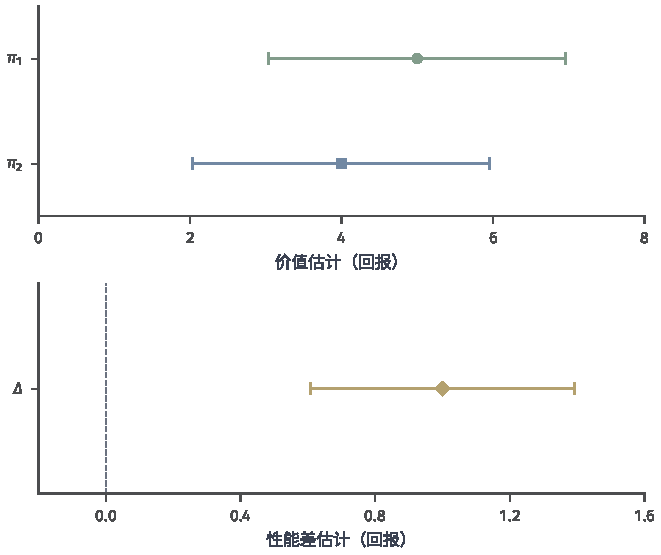
\includegraphics[width=112.000mm]{figures/10-reinforcement-learning/02-information-and-reward/matplotlib/rl-information-comparison.pdf}
  \caption{例~\ref{ex:rl-information-paired}~的教学区间。上组为两个价值的边际95\%正态近似区间，下组为共享轨迹计算的性能差区间；两组横轴各自标明量纲为回报。区间重叠与差是否包含0并非同一个判断。}
  \label{fig:rl-information-comparison}
\end{figure}

比较报告须列明候选数、产生候选所用的训练或评价记录、重复查询次数、置信水平和多重比较处理。候选集预先固定且有限时，可以分配各候选的失败概率，用并集界控制所有区间共同有效的事件；自适应增加候选不能直接沿用单候选区间。证据不足以排序时，就保留尚未排除的候选或报告无法排序。更多小数位不会增加证据。

% Outline: 4.4
\Needspace{35mm}
\section{固定经验下的策略学习与改进}
\label{sec:rl-information-offline-learning}

% Outline: 4.4.1
\subsection{策略学习的目标与数据边界}
\label{sec:rl-information-learning-boundary}

评价固定策略只检查指定行为，学习则要由日志生成新的候选。可以先以记录行为为拟合目标。\term{行为克隆}（behavioral cloning, BC）就是让策略在日志状态上给记录动作较高概率；在参数化策略类中，通过降低日志动作的平均负对数似然拟合参数：
$\min_{\bm\phi}\mathbb E_{\widehat P_D}[-\log\pi_{\bm\phi}(a\mid s)]$。
这一目标不使用奖励来重新分配概率。离线强化学习希望利用同一日志中的奖励选择行为，因此还要规定改进的比较基准。

拟合行为检查策略是否复现日志动作，提高估计回报检查学习目标是否上升。相对基线改进比较$J_H(\pi)$与$J_H(\pi_b)$，逼近最优则比较候选与允许策略类中最好的真实价值。后三者没有自动联系：优化器可能提高估计目标，却因查询日志未覆盖的动作而利用模型错误，降低真实回报。

\begin{example}[一次贪心更新利用了外推错误]
  \label{ex:rl-information-extrapolation}
  在单步教学任务中，日志只记录奖励为1的$a_0$；未记录的$a_1$真实奖励为$-10$。网络预测$\widehat Q(s,a_0)=1$、$\widehat Q(s,a_1)=5$，日志动作平方误差为0。按两个动作中的最大预测值作一次贪心更新，会选中$a_1$：估计回报从1升为5，真实回报从1降为$-10$。反复拟合原日志中的$a_0$仍不会提供$a_1$的正确后果。
\end{example}

行为克隆的目标可以用一个单状态例子看清：日志中$A$出现8次、$B$出现2次，设策略以概率$p$选$A$，平均负对数似然为$-0.8\log p-0.2\log(1-p)$，最小值在$p=0.8$。如果这两个动作的真实奖励分别为1和3，克隆策略期望奖励为$0.8(1)+0.2(3)=1.4$，而总选$B$能得3。这里两个动作都有记录，困难不是不可识别，而是拟合目标只复现动作频率，没有使用奖励来改进。

图~\ref{fig:rl-information-offline-pipeline}~把这类外推分成三个入口：策略生成新动作，价值备份查询新动作，规划器生成未观测状态动作。后续方法按限制这三个位置展开，也可组合使用。比较时保持训练记录与评价协议相同，说明优化对象、部署动作怎样产生以及额外假设；采用Transformer、扩散或流模型，并不单独说明策略是否改进。

\begin{figure*}[htbp]
  \centering
  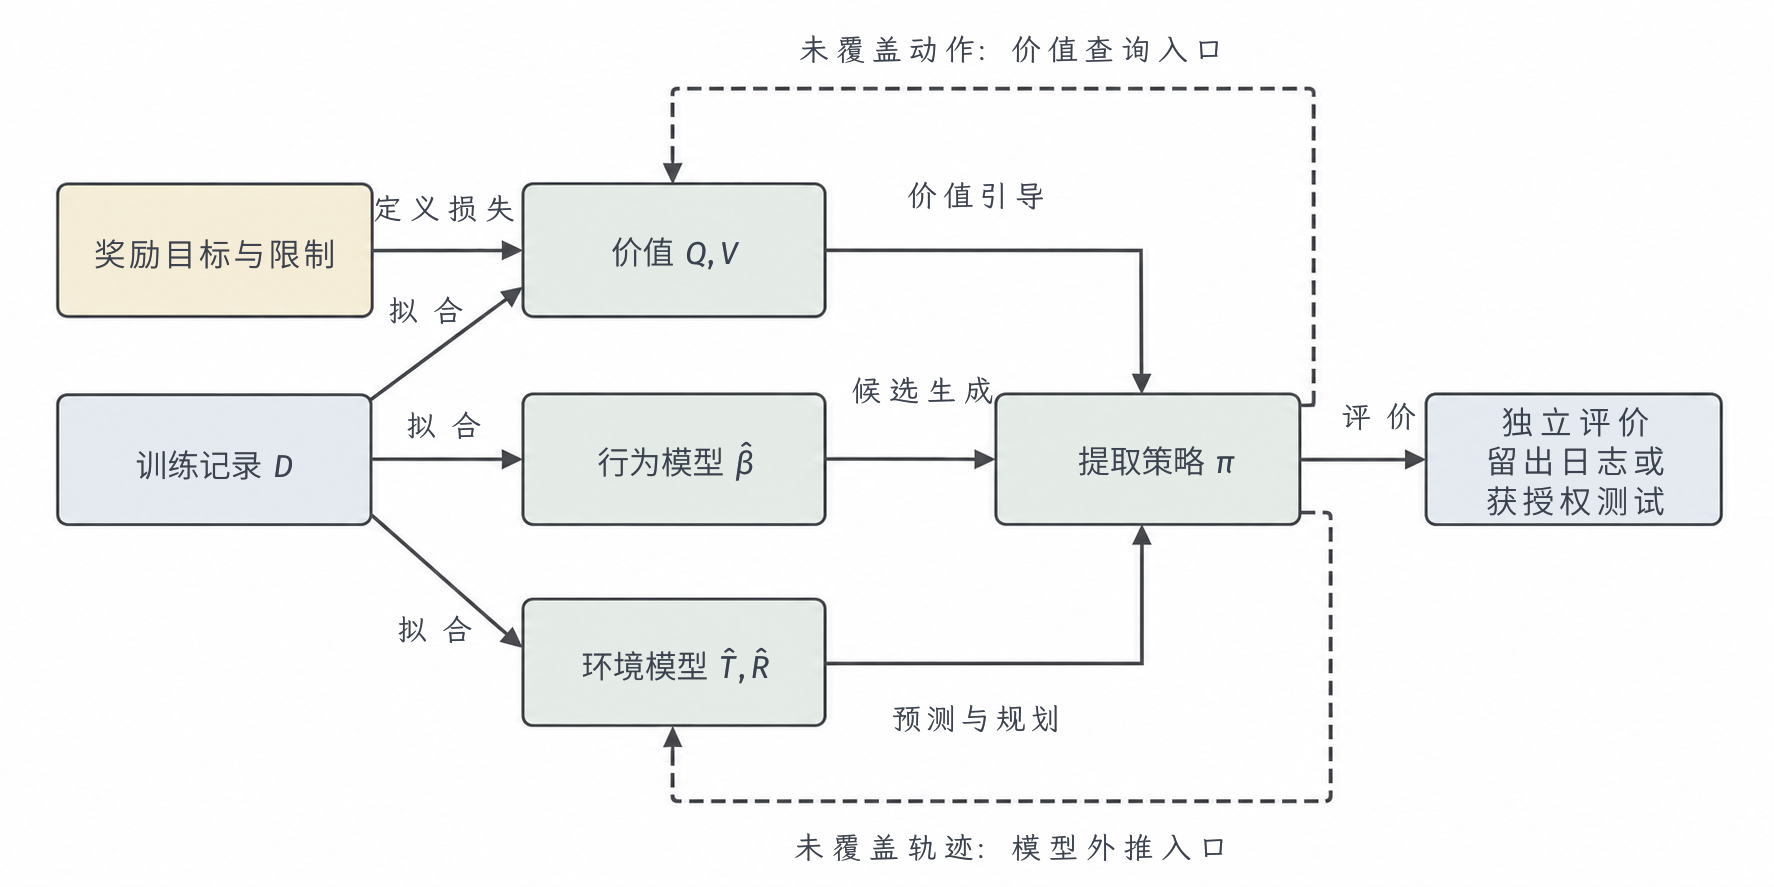
\includegraphics[width=157.400mm]{figures/10-reinforcement-learning/02-information-and-reward/generated/rl-information-offline-pipeline/figure.png}
  \caption{固定训练日志上的学习与评价。实线分别标注拟合、生成动作及评价，虚线标出外推可能进入的查询。行为约束限制动作来源，悲观价值限制对未支持动作的乐观估计，模型约束限制规划范围；任何一条学习路径仍需独立的评价证据。}
  \label{fig:rl-information-offline-pipeline}
\end{figure*}

% Outline: 4.4.2
\subsection{行为数据约束下的策略学习}
\label{sec:rl-information-behavior-constraint}

在例~\ref{ex:rl-information-extrapolation}~中，问题由策略选择未见动作触发，可以先约束候选偏离记录行为的程度。以下保持完全可观测与固定$D$，将价值目标改为无限折扣回报。TD3+BC沿用TD3的双评论家、目标网络和延迟行动者更新，在确定性行动者$f_{\bm\phi}(s)$的参数类中比较预测价值与动作平方偏差。对日志状态动作取平均，最大化价值减去偏差：
\begin{equation}
  \label{eq:rl-information-td3bc}
  \max_{\bm\phi}\ %
  \mathbb E_{(s,a)\sim\widehat P_D}
  \left[\lambda Q_{\bm\theta}(s,f_{\bm\phi}(s))
            -\lVert f_{\bm\phi}(s)-a\rVert_2^2\right].
\end{equation}
动作是向量时，范数比较各动作坐标，此处沿用动作符号$a$。为调节价值项与距离项的相对尺度，在含$N$条转移的一批训练记录上常取
$\lambda=\alpha/(\frac1N\sum_i|Q_{\bm\theta}(s_i,a_i)|)$，
其中$\alpha$控制相对强度，行动者更新时固定$\lambda$，分母为0时实现须有非零保护。按链式法则对行动者参数求梯度，可以看到两项各自推动动作的方向：
\[
  \mathbb E_{\widehat P_D}
  \left[(\nabla_{\bm\phi}f_{\bm\phi}(s))^\top
  \{\lambda\nabla_a Q_{\bm\theta}(s,a)|_{a=f_{\bm\phi}(s)}
          -2(f_{\bm\phi}(s)-a)\}\right].
\]
价值梯度推动动作朝预测价值较高处移动，距离梯度将它拉回记录动作。约束太弱可能再次利用外推，太强则接近模仿。两项的相对作用随奖励和动作尺度改变，因此比较$\alpha$必须同时给出归一化方式\scite{rl4-fujimoto2021-td3bc}

两项拉力也可手算。固定一个标量教学状态，记录动作$a=0$，暂设评论家曲线$Q(s,u)=-(u-0.6)^2$、$\lambda=1$。行动者若直接输出$u$，目标为$-(u-0.6)^2-u^2$，导数$1.2-4u$为0时得到$u=0.3$：它位于日志动作0与评论家峰值0.6之间。这只展示正则化怎样改变更新，不表示日志已证明0.3处的评论家预测正确。

平方距离还可能改变多模态行为的含义。另设左右绕障的路线参数为$-1$和1，日志各占一半，中间的0代表直行。单个确定性输出最小化平均平方偏差时得到0，却可能驶向障碍。复制均值并不等于复制两种合法路线的随机选择；这引出能够保留多个行为模式的动作生成器。

一种保留多个行为模式的办法是条件变分自编码器（conditional variational autoencoder, CVAE）。它用状态作为条件，用潜变量区分可能动作。训练时，编码器读取已记录的状态动作，将动作差别压进潜变量；解码器据状态与潜变量重构动作。部署没有待重构的真实动作，只能从先验抽潜变量，再由解码器产生候选。KL项使训练后验与采样先验保持联系，重构项让不同潜变量可以对应不同动作模式；两项都在拟合行为，不直接证明候选的真实回报。

若日志行为有多个动作模式，平方拟合可能得到模式之间日志记录稀少的均值动作。可以让行为模型生成不同模式，再在候选附近改进。\term{批量约束Q学习}（batch-constrained Q-learning, BCQ）以这种方式缩小价值筛选的动作范围。连续动作版本先在$(s,a)$记录上训练上述条件行为生成器，用$g_{\bm\omega}(s,\bm z)$表示解码器；生成候选时从规定潜变量先验采样，不再调用需要真实日志动作的编码器。随后由$\xi_{\bm\phi}(s,a)$给每个坐标加入$[-\Phi,\Phi]$内的扰动，$\Phi\geq0$，并截到合法动作域。生成$m$个候选后，仅按$Q_1$在这些修正候选中取最大值，得到执行动作：
\begin{equation}
  \label{eq:rl-information-bcq}
  a_j=g_{\bm\omega}(s,\bm z_j),\qquad
  \widetilde a_j=\operatorname{clip}_{\mathsf A}
                  (a_j+\xi_{\bm\phi}(s,a_j)),\qquad
  a_{\mathrm{exec}}\in\argmax_{\widetilde a_j,\ 1\leq j\leq m}
                  Q_1(s,\widetilde a_j).
\end{equation}

行为生成器以动作重构误差加潜变量后验相对标准先验的KL项训练。评论家备份也从下一状态生成$m$个候选，用目标网络的
$\eta\min(Q_1^-,Q_2^-)+(1-\eta)\max(Q_1^-,Q_2^-)$
评分，其中$\eta\in[0,1]$越大，越偏重两个评论家中的较小值。对候选取最高评分，构造$r_t+\gamma$倍继续价值的回归目标；真终止时后续为0。扰动网络在限幅内提高$Q_1$，目标网络缓慢更新。部署实际输出式~\eqref{eq:rl-information-bcq}~选中的动作，不是行为模型。候选数$m$为正整数，增加它会增加生成与价值计算；增大$\Phi$则放宽偏离日志的范围\scite{rl4-fujimoto2019-bcq}

例如，在一个标量教学状态下，生成器给出三个候选动作，依次为$-0.2$、$0.1$和$0.3$。扰动将它们改为$-0.15$、$0.1$和$0.25$，对应的$Q_1$评分依次为$0.4$、$0.8$和$0.6$，于是执行第二个动作$0.1$。这个筛选范围较小，却不说明三动作后果都已有充分记录：生成模型可能跨过日志缺少记录的动作区域，扰动也可能越出支持。BCQ限制的是最大化搜索范围，覆盖条件仍须检查。

其他行为正则方法也限制偏离，但度量和施加位置不同。\term{BEAR}（Bootstrapping Error Accumulation Reduction）旨在减少自举误差累积，用最大均值差异（maximum mean discrepancy, MMD）比较行动者与行为动作样本，即比较核特征中的分布均值，约束备份尽量少查询分布外动作；距离含义取决于核、样本和阈值\scite{rl4-kumar2019-bear}

这个距离先把动作映到一组用于比较分布的特征，再比较两组样本的平均特征。若只比较动作数值均值，等概率取$-1,1$与恒取0都会给均值0，无法辨别两种分布。采用更丰富的核特征，可以检查均值以外的模式差别；例如高斯核给相近动作较高相似度，远动作较低相似度。这里的核是比较动作相似性的函数，不是前面产生状态反馈的概率核。核与阈值决定能约束哪些差异，距离小仍不能证明动作后果都被日志覆盖。

\term{BRAC}（Behavior Regularized Actor Critic）考察行为正则化的行动者与评论家，比较将行为分布散度加入策略目标或价值递推的不同方式。\term{ReBRAC}（Revisited BRAC）重新考察这类设计，沿用TD3+BC，在行动者与评论家目标中分别调节行为惩罚，并检查网络、批量和归一化等实现因素。表~\ref{tab:rl-information-behavior-methods}~据此对照各自限制的位置；这些改动不增加真实转移记录\scite{rl4-wu2019-brac,rl4-tarasov2023-rebrac}

\begin{table*}[t]
  \centering
  \small
  \begin{tabularx}{\linewidth}{p{15mm}XXXX}
    \toprule
    方法 & 行为接近度 & 施加位置 & 执行动作来源 & 强度与代价 \\
    \midrule
    BEAR & 动作样本的核最大均值差异 & 行动者约束，间接限制备份 & 训练后的随机行动者；可对候选评分 & 阈值、核及拉格朗日权重；行为模型与样本比较 \\
    BRAC & 相对行为模型的KL等散度 & 策略正则，或同时进入价值递推 & 正则化行动者 & 散度权重；行为密度拟合误差 \\
    ReBRAC & 相对日志动作的平方距离 & 行动者及评论家目标的独立惩罚 & 确定性行动者 & 两处惩罚系数；日志记录的后继动作与实现配置 \\
    \bottomrule
  \end{tabularx}
  \caption{行为正则的不同位置。表中“接近”都不表示已经获得未见动作的真实后果；实际比较还需固定动作尺度、训练记录与选模预算。}
  \label{tab:rl-information-behavior-methods}
\end{table*}

还可以不用显式行为距离，改用回报条件区分日志中的动作模式。\term{Decision Transformer}是一种回报条件序列模型，将过去状态、动作与剩余回报按因果顺序编码，以监督动作预测拟合$\pi_{\bm\phi}(a_t\mid I_t,g_t)$。这里又回到有限时域，其常见条件为未折扣剩余回报$g_t=\sum_{k=t}^{H-1}r_k$，不是默认折扣$G_t$。部署由用户指定希望达到的$g_0$，每步扣去实际奖励，按$g_{t+1}=g_t-r_t$更新。训练中$g_t$描述已发生轨迹的结果，部署中它是目标愿望；条件相同不保证结果可实现\scite{rl4-chen2021-dt}

\begin{example}[回报条件不能控制外部随机结果]
  \label{ex:rl-information-return-conditioning}
  设单步教学任务的奖励与动作独立：公平硬币以$1/2$概率给1，否则给0。仅取回报1的轨迹训练条件动作模型，可以完全拟合成功轨迹记录；但部署持续输入目标1，成功概率仍为$1/2$。按结果条件化只排除了失败样本，并未得到能够改变成功概率的动作。
\end{example}

回报条件模仿由结果标签区分行为，显式距离约束则惩罚分布或动作偏离，二者目标不同。前者可以表示高回报轨迹中的动作模式，却要面对幸运随机结果、不可达目标和日志外状态。判断执行策略是否改进，仍需第~\ref{sec:rl-information-evaluation}~节的价值证据。

% Outline: 4.4.3
\subsection{价值估计与策略更新中的外推控制}
\label{sec:rl-information-pessimism}

例~\ref{ex:rl-information-extrapolation}~中的未见动作被高估，除了限制策略，也可以改变价值训练。\term{保守Q学习}（conservative Q-learning, CQL）对缺少日志记录支持的高价值增加惩罚，使策略不容易因这些预测而偏离日志\scite{rl4-kumar2020-cql}
这里保持无限折扣价值和固定训练记录，采用有限动作的一种常用形式。从所用价值函数类选择$Q$，最小化Bellman平方残差与保守正则之和。正则先对全部有限动作价值取指数、求和再取对数，使较高值有较大影响；再减去日志动作的平均价值，约束日志未覆盖的动作相对日志动作的乐观程度：
\begin{equation}
  \label{eq:rl-information-cql}
  \min_Q\
  \frac12\mathbb E_{\widehat P_D}\bigl[Q(s,a)-y(s,a,r,s')\bigr]^2
  +\alpha\mathbb E_{s\sim\widehat P_D^S}
       \left[\log\sum_{a'}e^{Q(s,a')}
                       -\mathbb E_{a\sim\widehat\beta_{D}}Q(s,a)\right].
\end{equation}
其中$\alpha\geq0$控制正则强度，$y$由固定目标网络$Q^-$构造。评价当前$\pi^{(k)}$时，按其下一动作分布取期望，可令
$y=r+\gamma\mathbb E_{a'\sim\pi^{(k)}(\cdot\mid s')}Q^-(s',a')$；
控制备份也可以使用规定的动作最大化版本，真终止处都将继续价值置0。
$\widehat\beta_{D}$是该状态下日志动作的经验分布。为检查正则修正的方向，对动作价值求导，得到
$\alpha(\operatorname{softmax}(Q)(a\mid s)-\widehat\beta_{D}(a\mid s))$；
于是无日志记录却预测很高的动作受到向下修正，日志动作得到相对支撑。连续动作不能直接枚举有限和，须按规定采样分布近似相应积分。

保守项可以看成让所有动作参与一次相对比较。Bellman回归只在日志动作上计算残差，未见动作的高预测可能没有任何修正；指数求和则会给高预测动作较大的梯度，再与日志动作频率相减。按动作价值坐标看，当某动作的softmax权重大于其日志频率时，沿保守项的负梯度更新会降低该动作的预测值。这是在控制策略容易利用的相对乐观程度，而非从未见动作获得真实负奖励标签。

沿用例~\ref{ex:rl-information-extrapolation}~的动作与日志，另设教学预测
$Q(a_0)=0,Q(a_1)=4$。未见$a_1$的正则梯度约为$0.982\alpha$，梯度下降会压低它。这解释了局部抑制机制，却不证明训练后所有$Q(s,a)$都是可信下界。CQL理论还依赖表格或特定逼近、采样误差、正则强度及策略更新条件；常用版本控制策略期望价值下界，不能扩大为每个动作的逐点下界。

也可以改变继续价值的计算，避免价值训练查询新行动者提出的日志未覆盖的动作。\term{隐式Q学习}（implicit Q-learning, IQL）从同一状态的日志动作价值中拟合偏向较高值的状态价值，再用它构造Q目标。要表达这种偏向，可用\term{期望分位数}（expectile）：以不对称权重计量高估和低估的平方误差，找出平均损失最小的位置。它不同于按概率质量切分的分位数，还考虑两侧偏差大小。对于平方可积的$X$和$\tau\in(0,1)$，比较所有实数位置$v$，定义
\begin{equation}
  \label{eq:rl-information-expectile}
  \ell_\tau(u)=|\tau-\mathbb I\{u<0\}|u^2,\qquad
  e_\tau(X)\in\argmin_v\mathbb E[\ell_\tau(X-v)].
\end{equation}
$\mathbb I$是指示函数，$u=X-v$为预测偏差。$\tau=1/2$使两侧权重相同，得到均值；$\tau>1/2$加重低估较大$X$的惩罚，使最优$v$向上移动。对离散分布求导，最优点满足
$\tau\mathbb E[(X-v)_+]=(1-\tau)\mathbb E[(v-X)_+]$。

先用一个状态的动作值观察IQL怎样改变拟合权重。我们先求上侧的状态价值$V$，再用$A(s,a)=Q(s,a)-V(s)$比较各日志动作。策略拟合时让优势较大的记录占更大权重，取$\exp(\lambda_{\mathrm{AWR}}A)$，其中$\lambda_{\mathrm{AWR}}\geq0$控制同一优势差被放大多少。它改变的是行为克隆中各记录的相对权重，后面再写成三组训练损失。

\begin{example}[三个动作的IQL更新与提取]
  \label{ex:rl-information-iql}
  在教学状态$s$，三个日志动作等频出现，目标Q值为0、1、3，取$\tau=3/4$。为找状态价值，先假设$v\in[1,3]$，将一项低估与两项高估按损失权重平衡：
  \[
    \tfrac34(3-v)=\tfrac14[(v-0)+(v-1)],
  \]
  解为$v=2$，确实落在假设区间；损失凸，故为全局最优点。对到达$s$的非终止转移，若奖励0.5、$\gamma=0.9$，继续价值便给出Q回归目标$0.5+0.9(2)=2.3$。

  提取策略时取$\lambda_{\mathrm{AWR}}=\log2$。三个优势$-2,-1,1$对应未归一化权重$1/4,1/2,2$。策略若可在所有分类分布中选择，则最大化加权对数似然等价于按等频日志动作的权重归一化，得到
  \[
    \pi(a_1\mid s)=1/11,\quad
    \pi(a_2\mid s)=2/11,\quad
    \pi(a_3\mid s)=8/11.
  \]
  若这些Q恰好等于单步真实奖励，提取策略的真实价值为$26/11$，高于等频行为的$4/3$，仍低于总选$a_3$的3。这一特殊情形也说明，拟合所得$V=2$不等于执行策略价值$26/11$。
\end{example}

在刚才的等频$0,1,3$例中，均值为$4/3$，$0.75$分位数为3，而$0.75$期望分位数为2。分位数只用两侧概率质量定位，期望分位数还平衡两侧距离，因而得到不同位置。IQL用上侧位置偏向较好的日志动作，再让策略更多拟合这些动作；随机奖励或随机后继仍由Q回归平均，不能把幸运结果也当成可选择的动作。

IQL在每个状态按日志动作的经验分布形成上述随机变量$Q(s,a)$。以下回到无限折扣价值，保持固定训练记录；$Q_{\bar{\bm\theta}}$为固定目标网络，$V_{\bm\psi}$为状态价值网络。先在各自参数类中最小化$L_V$拟合上侧位置，再最小化$L_Q$拟合奖励加继续价值，最后最小化$L_\pi$，用优势指数提高较好日志动作的拟合权重：
\begin{align}
  \label{eq:rl-information-iql}
  L_V(\bm\psi)
    &=\mathbb E_{(s,a)\sim\widehat P_D}
       \ell_\tau(Q_{\bar{\bm\theta}}(s,a)-V_{\bm\psi}(s)),\nonumber\\
  L_Q(\bm\theta)
    &=\mathbb E_{\widehat P_D}
       [Q_{\bm\theta}(s,a)-r-\gamma V_{\bm\psi}(s')]^2,\nonumber\\
  L_\pi(\bm\phi)
    &=-\mathbb E_{(s,a)\sim\widehat P_D}
       [\exp(\lambda_{\mathrm{AWR}}\widehat A(s,a))\log\pi_{\bm\phi}(a\mid s)],\\
  \widehat A(s,a)&=Q_{\bar{\bm\theta}}(s,a)-V_{\bm\psi}(s).
  \nonumber
\end{align}
每次更新将目标量固定，真终止时$V(s')=0$。$\lambda_{\mathrm{AWR}}\geq0$是逆温度，控制优势差怎样转为相对拟合权重。可先完成价值拟合再提取策略，也可交替训练，但策略梯度不反向改变价值目标。实践中还使用双Q较小值和权重截断，须报告阈值。上侧expectile施加在同状态的动作价值上，而Q平方回归仍平均奖励及随机转移，不挑选幸运反馈。原IQL用分开的$V$、$Q$目标保持了可选择动作与不可选择环境结果的区别\scite{rl4-kostrikov2022-iql}

\begin{algorithm}[固定经验上的IQL与策略提取]
  \label{alg:rl-information-iql}
  \begin{algorithmic}[1]
    \Require 固定$D$，$\gamma,\tau,\lambda_{\mathrm{AWR}}$，价值与策略更新预算，权重截断阈值
    \Ensure 可执行$\pi_{\bm\phi}$及训练、验证与最终评价记录的用途说明
    \State 初始化$Q_{\bm\theta},Q_{\bar{\bm\theta}},V_{\bm\psi},\pi_{\bm\phi}$
    \For{每次价值更新}
      \State 从$D$抽取转移批次，按$L_V$拟合日志动作Q值的expectile
      \State 按真终止标记屏蔽继续价值，构造固定目标$r+\gamma V_{\bm\psi}(s')$
      \State 按$L_Q$更新评论家，再缓慢更新目标Q参数
    \EndFor
    \For{每次策略提取更新}
      \State 固定价值网络，计算日志动作优势和截断后的指数权重
      \State 最小化加权负对数似然$L_\pi$
    \EndFor
    \State 固定提取策略，按第~\ref{sec:rl-information-evaluation}~节评价，不以$V$直接充当最终证据
  \end{algorithmic}
\end{algorithm}

算法~\ref{alg:rl-information-iql}~按给定更新预算先拟合价值，再用固定价值提取动作分布，最后将执行策略送往评价。表~\ref{tab:rl-information-extraction}~进一步对照提取方式：同一价值函数经不同动作来源形成不同策略，其逼近误差与覆盖风险也不同。

\begin{table*}[htbp]
  \centering
  \small
  \begin{tabularx}{\linewidth}{p{26mm}XXX}
    \toprule
    提取方式 & 动作来源与价值查询 & 逼近误差 & 覆盖风险 \\
    \midrule
    直接贪心 & 全动作优化或行动者提出动作；查询其Q值 & 动作优化不精确、评论家误差 & 容易主动寻找日志未覆盖的高估动作 \\
    优势加权拟合 & 用日志动作训练执行分布；训练查询日志动作的Q值 & 策略族与加权分布不匹配、优化误差 & 连续输出仍可能落在稀疏间隙 \\
    行为采样后筛选 & 生成$m$个候选，按Q取最大或重采样 & 行为生成偏差、有限$m$误差 & 生成概率非零不证明环境后果有支持 \\
    \bottomrule
  \end{tabularx}
  \caption{价值学习之后的三个动作接口。增大候选数或策略容量可能减少提取误差，也可能更充分地利用价值外推误差。}
  \label{tab:rl-information-extraction}
\end{table*}

扩散模型也可接入这些动作提取方式。

简单的单峰行动者可能难以拟合优势重加权后的多种动作模式。扩散动作模型从随机噪声开始，按学得的条件去噪步骤逐渐生成动作，借不同噪声样本保留多个模式。价值可以参与训练，使生成过程偏向高评分动作，也可以只在候选生成之后进行筛选。这两种连接改变的是梯度是否进入生成器，不能因为都生成动作就视为同一个策略更新。

\term{Diffusion-QL}（Diffusion Q-learning）将扩散动作建模与Q学习结合，拟合条件动作扩散模型，并在去噪目标外最大化生成动作的价值，让价值梯度经生成过程改变策略。行为建模与价值驱动训练由此结合，去噪步数则同时影响训练和推理成本\scite{rl4-wang2023-diffusionql}
\term{IDQL}（Implicit Diffusion Q-learning）将隐式Q学习与扩散动作模型结合，研究价值目标对应的行为重加权分布，以扩散行为模型生成候选，按评论家导出的权重重采样，或采用贪心提取变体。它试图减少简单行动者无法表示多模态隐含策略的误差；生成候选仍不提供新的环境后果证据\scite{rl4-hansenestruch2023-idql}

图~\ref{fig:rl-information-extraction}~区分价值梯度改变生成器与价值筛选已有候选。流模型也能通过可微变换把简单噪声变成动作分布，生成候选或提供动作映射；要据此说明改进，仍须接入有依据的价值加权、策略目标或规划准则。单独拟合条件生成模型没有完成这一比较步骤。

\begin{figure*}[htbp]
  \centering
  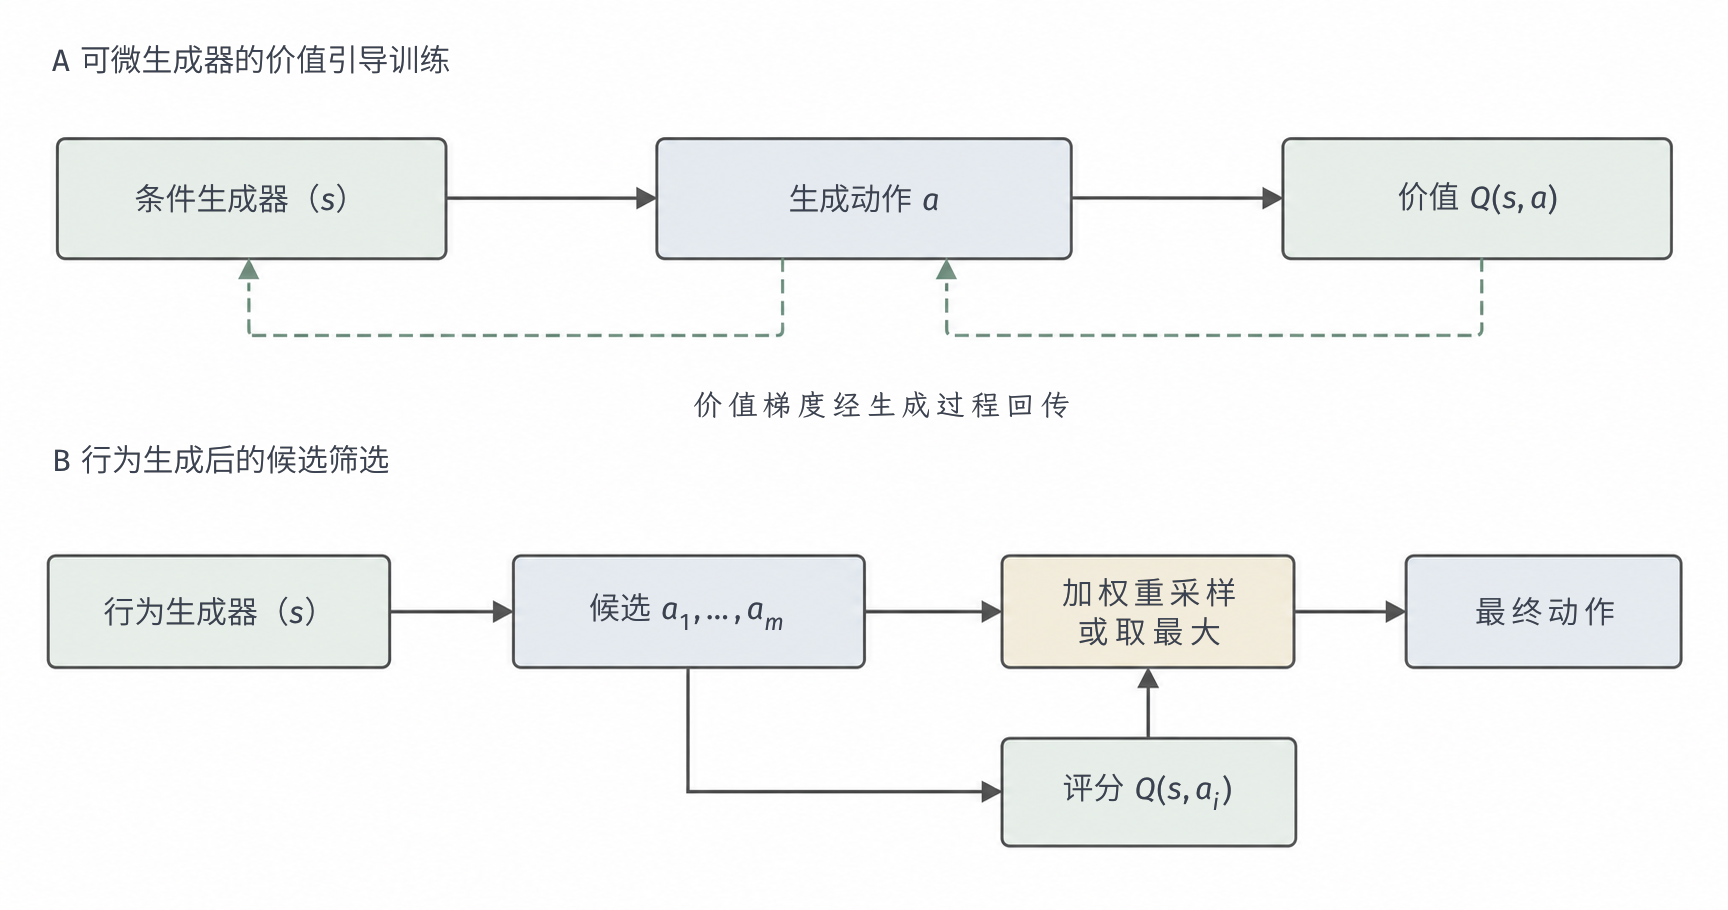
\includegraphics[width=157.400mm]{figures/10-reinforcement-learning/02-information-and-reward/generated/rl-information-extraction/figure.png}
  \caption{生成式动作的两种价值接口。实线表示动作生成、价值评价与候选选择。A的虚线将动作价值梯度经生成动作和可微生成过程回传到生成器；B把候选和对应评分分别送入筛选，再给出最终动作。A改变生成器，B筛选已有候选，两者属于不同的策略构造接口。}
  \label{fig:rl-information-extraction}
\end{figure*}

动作还可以组合为序列。近期\term{DEAS}（DEtached value learning with Action Sequence）研究动作序列上的价值学习，将其与显式行动者分离，以减轻动作块评价的过估计；其ICLR 2026正式版本研究长时程离线任务与动作序列模型。动作块减少显式选择次数，却扩大了组合动作空间；固定长度序列也不等于能够中途依反馈行动的Option，更不说明日志覆盖全部动作块。这里只将DEAS作为该接口的近期研究，基准表现不构成普遍最优性结论\scite{rl4-kim2026-deas}

% Outline: 4.4.4
\subsection{学习模型上的规划与策略优化}
\label{sec:rl-information-model-learning}

第~\ref{chap:rl-learning}~章允许新交互，因此规划器查询到模型的可疑预测后，还可采样校正；固定经验下无法这样验证。我们仍可从日志拟合$\widehat R(s,a)$和$\widehat T(s'\mid s,a)$，并计算不确定性分数$u(s,a)$。留出转移记录能检查其覆盖区域中的部分预测误差；日志未覆盖状态动作的真实后果却不能仅由小误差、小集成分歧或高似然证明。

\term{MOPO}（Model-based Offline Policy Optimization）在学习模型上进行离线策略优化，模型滚动时扣除不确定性惩罚：从日志状态出发，按当前策略在$\widehat T$中生成有限长度轨迹，以
$\widetilde R=\widehat R-\lambda u$作为模拟奖励，再混合真实与模拟转移更新策略并重复这一过程。模型只由真实$D$拟合，模拟转移保留来源标识。滚动长度控制误差可累积的范围，$\lambda$调节不确定区域的惩罚\scite{rl4-yu2020-mopo}

惩罚有两种不同含义。若$u$只是模型成员的分歧，扣去$\lambda u$会降低分歧大区域的评分，但成员也可能一致地错；这只是一项偏好调整。若能证明惩罚至少覆盖相关奖励和下一价值预测误差，扣除后才有依据称为保守下界。接下来把误差逐项写出来，说明这两个意义之间需要哪一步论证。

要把惩罚后的回报解释为真实价值下界，需要知道它扣除的量能否覆盖模型误差。固定$\pi$和无限折扣目标，令$\widehat d^\pi$为$\widehat T$下的归一化占用。为计算真实价值减去模型价值，将两个Bellman方程相减，并按模型轨迹的访问概率累积，得到
\begin{equation}
  \label{eq:rl-information-model-telescoping}
  J_M(\pi)-J_{\widehat M}(\pi)
  =\frac1{1-\gamma}\mathbb E_{\widehat d^\pi}
       \left[R-\widehat R
                  +\gamma(T-\widehat T)V_M^\pi\right].
\end{equation}
这里$(T-\widehat T)V$是两核给出的下一价值期望之差。共同$\mu_0$和有界价值使折扣尾项消失；占用已归一化，故保留$1/(1-\gamma)$。若在该策略访问区域内，
$|R-\widehat R|\leq u_R$且
$|(T-\widehat T)V_M^\pi|\leq u_T$，
则每处误差项不低于$-u_R-\gamma u_T$。按同一非负占用分布平均，得到扣除奖励与转移价值误差上界后的保守回报：
\[
  J_M(\pi)\geq
    \frac1{1-\gamma}\mathbb E_{\widehat d^\pi}
       [\widehat R-u_R-\gamma u_T].
\]
因此，$\lambda u$只有与实际误差上界建立联系，才具有上述下界含义。用它选择策略时，条件还须同时覆盖参与选择的候选，不能沿用单个预固定策略的界。所有集成模型也可能一致地学错；没有覆盖或正确结构支撑时，模型分歧仍只是启发式诊断。

除惩罚奖励外，\term{MOReL}（Model-Based Offline Reinforcement Learning）也是基于模型的离线强化学习方法，在不可信状态动作处转入低回报吸收状态，使规划器少离开可信区域\scite{rl4-kidambi2020-morel}
\term{COMBO}（Conservative Offline Model-Based Policy Optimization）在学习模型上进行保守离线策略优化，对模型滚动状态动作施加保守价值正则，不必先构造同一种显式不确定性分数\scite{rl4-yu2021-combo}
两者都仍需要真实交互记录和各自保证中的模型误差条件。表~\ref{tab:rl-information-model-methods}~在相同日志缺口下比较这些选择：未见动作若实际很好，保守限制会放弃可实现回报；若实际很差，限制可能阻止规划器利用错误预测。

\begin{table*}[t]
  \centering
  \small
  \begin{tabularx}{\linewidth}{p{17mm}XXXX}
    \toprule
    方法 & 限制位置 & 候选轨迹来源 & 真实交互记录依赖 & 保守程度与代价 \\
    \midrule
    MOPO & 模型奖励减去误差代理惩罚 & 日志状态出发的短模型滚动 & 动力学拟合及误差校准 & 惩罚系数、滚动长度；可能拒绝高回报稀疏区域 \\
    MOReL & 不可信区域进入低回报吸收态 & 悲观模型中的规划或学习 & 可信区域判定与模型置信 & 阈值与吸收惩罚；错误拒绝会缩小可达策略类 \\
    COMBO & 真实交互与模型生成转移上的保守价值正则 & 学习模型中的策略滚动 & 模型拟合及日志动作的价值支撑 & 正则及混合比例；过强会压低真实可行动作 \\
    \bottomrule
  \end{tabularx}
  \caption{模型法限制外推的三个位置。比较成立的前提是任务、日志、模型容量与查询预算相同；减少显式不确定性估计不等于不再需要误差依据。}
  \label{tab:rl-information-model-methods}
\end{table*}

另一种模型使用方式是直接生成整段轨迹。\term{Trajectory Transformer}是一种轨迹序列预测模型，自回归地预测状态、动作与奖励序列，规划时用束搜索保留高评分候选，再执行选中轨迹的首个动作；收到真实观测后重新搜索。改进还取决于搜索评分与候选可行性，不能仅由下一token预测损失推出。
\term{Diffuser}用扩散模型进行轨迹规划，按当前状态等条件，通过回报引导的扩散采样形成计划，也可执行首个动作后滚动重规划。前者搜索自回归候选，后者引导去噪生成计划，但两者轨迹都是模型预测，没有增加观测经验\scite{rl4-janner2021-trajectory,rl4-janner2022-diffuser}

部署接收反馈并重规划，不说明训练期间有在线调参权限。若为选超参数反复在真实环境执行计划，这些查询须计入第~\ref{sec:rl-information-limited-interaction}~节的新增预算。搜索与模型滚动的通用计算见第~\ref{chap:rl-planning}、\ref{chap:rl-learning}~章；固定日志下，规划器仍不能自行验证日志未覆盖区域的模型预测。

% Outline: 4.4.5
\subsection{策略改进的保证与比较}
\label{sec:rl-information-improvement}

前述三类限制都产生了候选，但候选价值超过估计基线还不等于真实改进。需要先规定比较哪些策略，以及估计误差能否同时约束它们。下面固定候选集合与基线，用共同误差事件计算选择后策略最多可能损失多少回报，不依赖特定网络或优化器。

\begin{theorem}[共同误差事件上的基线性能控制]
  \label{thm:rl-information-improvement}
  固定任务、初始分布、时域口径、非空候选策略集合$\Pi$及基线$\pi_b$，并假设所涉真实价值与估计值均为有限实数。给定$\varepsilon\geq0$；在日志与算法随机性所定义的概率空间上，若可测事件$C_{\mathrm{conf}}$中每个
  $\pi\in\Pi\cup\{\pi_b\}$均满足
  $|\widehat J(\pi)-J(\pi)|\leq\varepsilon$，且从$\Pi$中选出的可测策略$\widehat\pi$满足
  $\widehat J(\widehat\pi)\geq\widehat J(\pi_b)$，则该事件中真实价值满足
  \[
    J(\widehat\pi)\geq J(\pi_b)-2\varepsilon.
  \]
  若另给定$\delta\in[0,1]$且$\mathbb P(C_{\mathrm{conf}})\geq1-\delta$，结论也以至少$1-\delta$的概率成立。
\end{theorem}

\begin{proof}
  为把估计上的选择规则转为真实价值比较，在共同事件内插入候选和基线的估计值：
  \[
  \begin{aligned}
    J(\widehat\pi)
    &\geq\widehat J(\widehat\pi)-\varepsilon\\
    &\geq\widehat J(\pi_b)-\varepsilon\\
    &\geq J(\pi_b)-2\varepsilon.
  \end{aligned}
  \]
  第一、三步分别使用$\widehat\pi$与$\pi_b$的共同误差界，第二步使用选择规则。事件$C_{\mathrm{conf}}$发生时这条链必成立，故结论概率不低于$\mathbb P(C_{\mathrm{conf}})$。
\end{proof}

这一界允许真实回报比基线低$2\varepsilon$，并不保证严格提高。将选择阈值提高到
$\widehat J(\widehat\pi)-\widehat J(\pi_b)>2\varepsilon$，同样推导才给出严格正的真实增量。共同事件是关键条件：预固定单策略的95\%区间不能直接约束从许多候选中选出的最好者；候选集若由评价记录生成，还须处理适应性。

两侧误差可以先用数值检查。若候选估计价值为0.8、基线为0.7，二者误差各不超过0.1，允许的真实值仍包括候选0.7、基线0.8；估计领先0.1不能保证真实领先。候选估计领先必须严格超过0.2，才能排除两侧误差同时取最不利方向。这说明阈值不是任意保守系数，而来自比较时两份估计都可能出错。

共同误差界也可以进入候选策略的构造。若估计备份高的动作恰好也是日志稀少的动作，直接贪心可能选中正向估计误差；可以先扣除覆盖该误差的不确定性半径，再比较动作。\term{悲观值迭代}（pessimistic value iteration, PEVI）按这个思路反向规划。

一个单步教学例能显示扣除半径的作用。两个动作的奖励均值估计为$(0.6,0.8)$，假设已证有效的半径为$(0.05,0.4)$，悲观值就是$(0.55,0.4)$，于是选择第一个动作。若真实均值为$(0.58,0.4)$，两项绝对误差均在给定半径内；直接按估计贪心会选第二个动作，损失$0.18$，悲观选择则没有损失。此时最优动作半径给出的界为$2(0.05)=0.1$。这些构造值不提供半径有效性的统计证明；实际还须根据采集协议、模型或函数类证明共同事件。最优策略访问处缺少证据时，半径仍可很大，界也会很宽。表格或线性模型中成立的半径构造，不能仅凭同样使用悲观惩罚就移给深度CQL。

为明确其保证，改用完全可观测、时间齐次的有限MDP：$S,\mathsf A$有限非空，$H$为正整数，$t=0,\ldots,H-1$，$0\leq r_t\leq1$，不折扣，终端价值为0。日志$D$来自该MDP并保留完整转移字段；采集协议及算法随机性规定下述概率空间。真实备份作用于$v:S\to\mathbb R$：
\[
  (\mathcal B_t v)(s,a)
    =R(s,a)+\sum_{s'}T(s'\mid s,a)v(s').
\]

这项反向规划与在线探索的乐观备份方向相反。在线时，可以暂按较高价值尝试不确定动作，再用新经验修正；固定日志无法补试，因而先扣除误差半径，避免把未证实的好处当成行动依据。没有样本的动作需要用完整可能回报范围给大半径，不能因无法计算样本误差就设为0。下面的更新把固定日志不能补采记录的限制转成可计算目标。

从$\widehat V_H=0$按$t=H-1,\ldots,0$反向计算时，由同一训练日志$D$构造备份估计$\widehat m_t(s,a)$和非负半径$u_t(s,a)$。表格实现可以对相应$(s,a)$转移记录中的$r+\widehat V_{t+1}(s')$求平均，估计一次动作的奖励加继续价值；没有记录时，可例如约定$\widehat m_t(s,a)=0$、$u_t(s,a)=H-t$，用完整剩余回报范围覆盖未知备份，不能把缺失当作零误差。需要一个概率至少为$1-\delta$的共同可测事件$C_{\mathrm{pess}}$，其中$0<\delta<1$，使下式对所有$s\in S$、$a\in\mathsf A$及$t=0,\ldots,H-1$同时成立：
\begin{equation}
  \left|\widehat m_t(s,a)
       -(\mathcal B_t\widehat V_{t+1})(s,a)\right|
       \leq u_t(s,a).
  \label{eq:rl-information-pevi-confidence}
\end{equation}
这里$\widehat V_{t+1}$本身由$D$递归生成，误差界必须涵盖这一依赖；只对事先固定的$v$给出逐点置信区间还不够。减去半径后，再把数值截到剩余回报的允许范围：
\begin{equation}
  \begin{aligned}
    \widehat Q_t(s,a)
      &=\min\{H-t,\max\{0,\widehat m_t(s,a)-u_t(s,a)\}\},\\
    \widehat V_t(s)&=\max_{a\in\mathsf A}\widehat Q_t(s,a).
  \end{aligned}
  \label{eq:rl-information-pevi-backup}
\end{equation}
令$\widehat\pi_t(\cdot\mid s)$只给最大化动作分配概率，即每一步都对$\widehat Q_t$精确贪心。双侧误差界及截断使残差$(\mathcal B_t\widehat V_{t+1})(s,a)-\widehat Q_t(s,a)$位于$[0,2u_t(s,a)]$。若$V_t^\pi(s)$表示该有限MDP中从$s$起的剩余期望回报，$\pi^*$为全部时变马尔可夫策略中的最优者，则在$C_{\mathrm{pess}}$内，对每个初态$s$都有
\begin{equation}
  V_0^*(s)-V_0^{\widehat\pi}(s)
     \leq2\sum_{t=0}^{H-1}
       \mathbb E_{\pi^*}\!\left[u_t(s_t,a_t)\mid s_0=s\right].
  \label{eq:rl-information-pevi-gap}
\end{equation}
非负残差及精确贪心先给出$\widehat V_t\leq V_t^{\widehat\pi}$，因此控制$V_0^*-\widehat V_0$足以控制真实策略损失。再把$V_t^*-\widehat V_t$沿$\pi^*$的后继状态递推展开，每步残差至多为$2u_t$，便得到式~\eqref{eq:rl-information-pevi-gap}。所以右侧期望沿真实环境中的最优策略轨迹计算，已经取得的$D$及其半径保持固定；它不是把半径沿学得策略平均，也不是无条件的严格改进\scite{rl4-jin2021pessimism}。

也可以在候选形成时保留基线对日志记录稀少的状态动作区域的行为。\term{SPIBB}（Safe Policy Improvement with Baseline Bootstrapping）用基线自举约束策略改进，即日志记录稀少处沿用基线，其他动作才重新分配概率。有限MDP中以计数阈值$N_{\min}$识别稀少对，令
$\mathcal U_{\mathrm{rare}}=\{(s,a):N(s,a)<N_{\min}\}$，
其中$N(s,a)$为日志中的状态动作计数。要求$\mathcal U_{\mathrm{rare}}$内$\pi(a\mid s)=\pi_b(a\mid s)$，在其余动作上优化经验模型价值。例如基线动作概率$(0.6,0.3,0.1)$的第三项稀少，则保持0.1，而不是删去它再归一化；剩下0.9的概率可以在前两项间调整。

原始$\Pi_b$-SPIBB界依赖有限状态动作、有界奖励、已知且可执行的基线、按计数建立的模型置信条件及规定的受约束求解，控制的是相对基线容许损失。损失还随置信半径、折扣累积和经验模型增益变化，所以名称中的“安全”不表示每次运行超过基线。神经网络近似、模型误设或基线概率错误都不能直接继承表格结论\scite{rl4-laroche2019-spibb}

\begin{table*}[t]
  \centering
  \small
  \begin{tabularx}{\linewidth}{p{28mm}XXX}
    \toprule
    共同报告项 & 行为克隆 & 可复现行为策略 & 等预算离线改进方法 \\
    \midrule
    价值证据 & 留出OPE或独立测试；不是拟合准确率 & 原始版本、真实测试或日志回报及其条件 & 同一评价器、置信处理和查询权限 \\
    偏离与悲观设置 & 模型容量、拟合与执行动作的产生方式 & 原收集分布与版本 & 行为惩罚、价值惩罚、模型可信阈值 \\
    训练成本 & 训练记录遍历、批大小、更新次数 & 复现基线所需成本单列 & 评论家、生成器、模型及调参总成本 \\
    推理成本 & 一次动作预测或采样 & 原控制器调用成本 & 候选数、去噪步数、搜索与滚动长度 \\
    \bottomrule
  \end{tabularx}
  \caption{方法比较的报告口径，而非虚构的实验结果表。真实测试、离线估计和理论性能界分别标注，不能放在同一列中当作等强度证据。}
  \label{tab:rl-information-reporting}
\end{table*}

表~\ref{tab:rl-information-reporting}~将训练收益、证据类型及成本分别报告。基线本身可能回报很低，也可能违反业务安全要求，因此接近基线既不表示接近全局最优，也不说明满足碰撞概率或资源成本约束。基线性能界只控制给定条件下的相对回报；执行安全和约束保证由第~\ref{chap:rl-trustworthy}~章展开。

% Outline: 4.5
\section{有限新增经验下的策略修正}
\label{sec:rl-information-limited-interaction}

回到定理~\ref{thm:rl-information-unseen-action}~，原日志只含$a_0$的零奖励，无法区分两环境。若权限放宽，执行一次$a_1$，确定性奖励$+1$或$-1$便能排除一个解释。这里新增的是实际动作后果，而非一次模型预测。奖励有噪声时，一次查询通常还不能辨清环境，获得查询权限也不意味着估计误差已经可忽略。

这种追加交互记录的做法必须服从每轮协议：开始前声明可执行策略、步数、重置次数、专家帮助权限和验证用途。专家动作与主动随机探索的选择机制不同，新增日志要记录实际机制。即使用于最终报告而不参与梯度更新，试跑也消耗真实交互预算。

新经验加入后，原离线保守构造也要随证据重查。行为约束过强会挡住已有新增交互记录支持的动作，突然取消又可能让尚未校准的评论家驱动危险外推。\term{AWAC}（Advantage Weighted Actor Critic）采用优势加权的行动者与评论家设计，将离线与在线经验用于优势加权动作拟合，减少对显式行为密度的依赖\scite{rl4-nair2021-awac}
IQL也可将新经验接入原有$V,Q$与加权策略计算。\term{Cal-QL}（Calibrated Q-Learning）通过校准Q价值处理保守初始化的数值尺度：在下估当前策略价值时，用参考策略价值限制过度压低，减少微调初期仅为恢复尺度所作的更新。这是价值尺度校准，不是任意任务的概率校准保证\scite{rl4-nakamoto2023-calql}

\begin{table*}[t]
  \centering
  \small
  \begin{tabularx}{\linewidth}{p{18mm}XXXX}
    \toprule
    起点 & 新旧经验混合 & 评论家变化 & 行为限制变化 & 探索恢复要点 \\
    \midrule
    AWAC & 旧日志与在线回放用于动态规划和优势拟合 & 用当前继续策略的价值更新优势 & 加权似然的隐式接近度随训练记录改变 & 行动者必须真正产生可补足覆盖的新动作 \\
    IQL微调 & 新转移加入价值和策略训练 & 日志动作expectile与Q目标随新分布变化 & 温度、截断和混合比例决定偏离程度 & 不查询日志未记录动作的Q值不等于主动探索已经充分 \\
    Cal-QL & 离线初始化后混合在线经验 & 参考价值校准限制过度低估 & 保守强度与新证据一起检查 & 减轻初始价值尺度失配，仍需覆盖新增行为 \\
    \bottomrule
  \end{tabularx}
  \caption{有限交互修正中的组件职责。三行不是新的互斥算法分类；混合比例、约束强度和探索预算都需报告，不能只比较最终训练步数。}
  \label{tab:rl-information-finetuning}
\end{table*}

表~\ref{tab:rl-information-finetuning}~列出的组件可以接入同一轮修正。算法~\ref{alg:rl-information-round}~先采集新增交互记录并更新训练记录组，再形成候选，最后重新评价。新经验同时改变覆盖与行为分布，所以旧评价器的概率和误差条件也需要重新核对。

\begin{algorithm}[一轮有限经验修正]
  \label{alg:rl-information-round}
  \begin{algorithmic}[1]
    \Require 当前日志$D^{(k)}$、基线、候选，收集预算$B_k$与独立评价预算$E_k$
    \Ensure 更新后的候选集合与本轮证据支持的回报比较结论
    \State 固定本轮收集策略及版本，声明可访问状态、重置和帮助权限
    \State 在$B_k$内收集经验，保存策略概率、轨迹边界及用途标识
    \State 构成$D^{(k+1)}$，重新检查覆盖及新旧交互记录的混合权重
    \State 更新表示、价值模型、行为模型或转移与奖励模型，按选定接口提取候选
    \State 固定待比较策略，在保留日志或$E_k$内的独立交互上重新评价
    \State 依据置信规则保留、替换或拒绝候选，记录下一轮需补采的状态动作、奖励或行为概率字段
    \State 扣除收集、验证、重置及专家调用预算；预算用尽时停止
  \end{algorithmic}
\end{algorithm}

新增经验有两个可能用途：帮助排除环境解释，或检验一份已经固定的策略。前者可以随已观察反馈调整下次查询，后者需要保持待评价策略和统计目标不变。若一边看分数一边改策略，得到的是适应过程的记录，不能直接作为最终固定策略的独立测试；两种用途都要计入真实查询预算。

除了总预算，协议还决定动作能否根据上一批反馈改变。下面在相同两次查询下，只改变反馈可以进入决策的轮次。

\begin{example}[相同两次查询与不同适应轮次]
  \label{ex:rl-information-batches}
  沿用两个单步环境：$a_0$奖励0，$a_1$分别恒为$+1$或$-1$。为教学比较，假设先验各为$1/2$，共允许两个新回合，每回合一次动作。

  两次动作若都须在取得反馈前确定，预先选几次$a_1$都使两环境的平均收集回报为0。允许分两轮时，可先执行$a_1$，正奖励后再选$a_1$，负奖励后改选$a_0$；两环境总回报为2和$-1$，先验平均为$1/2$。
\end{example}

这项差距属于收集期间总回报，不是所有最终指标的差距。若只要求收集结束后确定动作，一次性设计中安排一次$a_1$也可辨认环境。相同样本预算配合不同反馈时机，仍可能产生不同的行动过程，因此多轮方法须报告原日志、每轮新增预算和反馈使用时机，并将反复测试的选择偏差纳入证据处理。

% Outline: 4.6
\section{两类信息限制叠加时的强化学习}
\label{sec:rl-information-combined}

% Outline: 4.6.1
\subsection{两类限制下的决策目标与可用信息}
\label{sec:rl-information-combined-target}

此前讨论了怎样用历史表示处理执行时状态不可见，离线评价则暂时假设日志记录完整状态。现在撤掉完整状态假设并保留固定经验：日志中的历史未必包括收集者实际使用的所有线索。因此，不能只将评价式中的$s_t$换成$\bm z_t$。需要先固定目标量，再分别核对执行策略可读取的历史、日志实际保存的字段和采集者选动作时读取的观测或状态。

以下恢复有限时域$H$，固定$\mu_0$、$0\leq\gamma<1$和执行可得历史$I_t$，以$\Pi$表示允许的历史策略类。可以针对一个$J_H(\pi)$、两个候选的差或相对基线增益提出问题；若要找$\Pi$内的最优行为，就需要比较全部相关候选。一个候选可评价，只回答该候选的问题，不足以推出能够找到全局最优。

\begin{table*}[htbp]
  \centering
  \small
  \begin{tabularx}{\linewidth}{XXX}
    \toprule
    执行策略可读历史 & 日志实际字段 & 采集者选动作的依据 \\
    \midrule
    只见位置与历史动作、奖励 & 同样的全回合历史与边界 & 同样历史及独立随机数：可建立历史条件校正 \\
    可以保留起始提示 & 日志只保留最近窗口 & 收集者记住提示：执行策略所需的历史未被日志完整保存 \\
    只见传感观测 & 记录动作概率但缺少概率所条件化的上下文 & 专家还看到未记录状态：不能把边缘频率当成随机分配机制 \\
    回合开始重置记忆 & 片段无回合标识、无前缀 & 行为控制器跨片段保留记忆：初始化机制未知 \\
    \bottomrule
  \end{tabularx}
  \caption{离线POMDP中的三类不同的决策依据与记录字段。动作概率需要连同它所依据的历史字段和收集协议解释；一个额外字段不能自动修复全部缺口。}
  \label{tab:rl-information-information-sets}
\end{table*}

表~\ref{tab:rl-information-information-sets}~第二行的日志缺少部署可保留的提示，因而无法重建待评价策略所需的可得历史；第三行缺少专家选动作的依据，还可能改变动作分组与结果之间的统计关系。这两种遗漏分别涉及隐藏状态与未记录的采集依据，却阻断评价的不同步骤。要判断模型是否足够，应按当前价值或动作比较检查，而非要求恢复所有隐藏状态名称。

例如，交换隐藏状态名称会改变参数表示，却不改变任何可执行策略的价值，控制无需唯一的隐藏语义。两个同样预测原日志的模型则可能在强制执行别的动作后给出不同后果；这种差异会改变策略判断。先声明目标结论，才能确定哪些模型差异必须识别。

\begin{definition}[给定问题上的决策等价]
  \label{def:rl-information-decision-equivalence}
  决策等价以给定的允许策略类、时域、初始条件与目标结论为条件。两个潜在模型若对该问题涉及的全部价值或动作比较给出相同结论，则在该问题上决策等价。该等价不要求隐藏状态名称一致，也不延伸到未声明的新奖励或策略类。
\end{definition}

% Outline: 4.6.2
\subsection{策略结论的可识别程度}
\label{sec:rl-information-identification-levels}

以表~\ref{tab:rl-information-information-sets}~为起点，离线POMDP至少要核对三个条件。日志应完整保留执行策略所需的观测、历史动作和奖励并具有正确回合边界；行为应只依据记录历史和独立随机化，或满足另一个明确识别条件；目标历史动作应有行为支持。物理状态隐藏不等于行为机制不明：控制器若也只见记录历史，隐藏状态虽影响反馈，却没有额外进入动作选择。

日志未必能对每个目标都满足这些条件。为了说明已记录字段的总体分布与结构假设到底排除了哪些模型，可以把具有同一可观测总体分布、又满足既定结构假设的模型保留下来，再查看它们对目标量给出了哪些答案。

可以回接只记录$a_0$零奖励的单步例子。若事先允许$a_1$的奖励为$[-1,1]$内任意数，那么每个不同奖励都对应一份与日志相容的环境。即使选一个网络给$a_1$预测0.4，其他相容环境也没有被日志排除。需要保留的是所有尚未排除的解释，以及它们对问题给出的答案；多次初始化得到的几个网络，并不自动代表这个完整集合。

\begin{definition}[一致模型集合与识别集合]
  \label{def:rl-information-identified-set}
  给定可观测日志总体分布$p_{\mathrm{obs}}$与结构假设集合$\mathcal A_0$，一致模型集合定义为
  \[
    \mathcal M(p_{\mathrm{obs}},\mathcal A_0)
       =\{M:M\text{满足}\mathcal A_0
                  \text{且产生}p_{\mathrm{obs}}\}.
  \]
  每个$M$同时指定潜在环境与相容的记录生成机制。将目标量$\theta_{\mathrm{tar}}(M)$在这些模型中的取值收集为识别集合
  $\mathcal I_{\mathrm{tar}}=\{\theta_{\mathrm{tar}}(M):M\in\mathcal M\}$，假设$\mathcal M$非空。
  $\mathcal I_{\mathrm{tar}}$为单元素时，$\theta_{\mathrm{tar}}$被点识别；若非单元素但严格包含在预先允许范围内，则得到部分识别。对于策略排序，需单独检查所有允许模型是否给出相同次序；若存在相反排序，则排序不可识别。
\end{definition}

这里$\theta_{\mathrm{tar}}$表示要回答的目标数字，如某策略的回报或两策略的回报差，不是训练参数。$\mathcal M$收集尚未排除的环境及收集机制，$\mathcal I_{\mathrm{tar}}$则把这些解释转成可能答案。若所有解释给同一个数，答案唯一；若只知道一个范围，还要看当前决策是否真的需要精确数值，还是只需知道差的符号。

确定数值与确定决策是不同要求。例如，性能差$\theta_{\mathrm{tar}}(M)=J_M(\pi_1)-J_M(\pi_2)$若原可取$[-10,10]$，日志和结构将其缩小到$[-1,2]$，便已缩小了目标量的可取范围，但正负值仍并存，不能排序。若缩小到$[1,2]$，数值仍未唯一确定，符号却足以说明$\pi_1$较好。下面按目标是否点识别、是否只有部分范围、是否仍不能回答决策展开；部分识别本身不等于无法决策。

一致模型和识别集合描述总体分布已知时的限制，有限日志还会引入采样误差，需要再构造相应目标量或识别集合的统计置信集合。一个模型拟合有限日志很好，既没有排除其他总体相容模型，也没有单独控制采样误差。

接下来将专家与部署者看到的线索分开。专家知道类型$U$，部署者却只看见相同画面；专家因此可能只在某种类型下选$a_0$，只在另一种类型下选$a_1$。日志中两组奖励的比较就同时改变了动作与类型。表中的$r(a_0),r(a_1)$表示某类型若分别执行两个动作会得到的奖励，未选动作的数值是教学模型的构造假设，不能从实际日志直接读出。我们用两份不同构造检验：保留下来的实际记录相同，是否仍能有相反的部署价值。

\begin{example}[同样日志与相反的动作价值]
  \label{ex:rl-information-confounding}
  构造单步教学任务，观测$o$恒定，类型$U\in\{0,1\}$等概率且未记录，专家却能看到它。下面给出两个模型中专家的动作和每种类型执行两动作的潜在奖励：
  \[
  \begin{array}{cc|c|rr}
    \text{模型}&U&\text{专家动作}&r(a_0)&r(a_1)\\
    \hline
    M_+&0&a_0&1&3\\
    M_+&1&a_1&-1&1\\
    M_-&0&a_1&3&1\\
    M_-&1&a_0&1&-1
  \end{array}
  \]
  两模型都以$1/2$记录$(o,a_0,1)$、以$1/2$记录$(o,a_1,1)$。部署看不到$U$，若始终选一个固定动作，其价值须按总体类型概率平均该动作后果，而非只平均专家选它的类型：
  \[
  \begin{array}{c|rr}
    &J_1(\pi_{a_0})&J_1(\pi_{a_1})\\
    \hline
    M_+&(1-1)/2=0&(3+1)/2=2\\
    M_-&(3+1)/2=2&(1-1)/2=0
  \end{array}
  \]
  因此，相同记录分布在两模型中对应相反的最优固定动作。
\end{example}

只用$o$拟合动作频率，会得到$\widehat\beta(a_0\mid o)=\widehat\beta(a_1\mid o)=1/2$。用它作普通IS，对任一固定动作目标都算得
$(1/2)\times2\times1=1$，既不是0也不是2。边缘上两动作都出现，并未恢复条件随机化：专家选该动作的样本只来自特定类型，不能代表总体类型执行该动作的结果。

行为机制是否含有额外隐藏依据，是其中一个关键区别。\term{隐藏混杂}（hidden confounding）指未记录变量同时影响动作选择与后果，观察到的动作组因而不能直接代表随机试验组。图~\ref{fig:rl-information-confounding}~对照普通隐藏状态与这种共同原因；箭头是声明的因果生成假设，不是拟合日志自动发现的事实。只有在行动前的共同历史足以阻断采集动作与潜在后果的额外联系，并且目标行动有相应支持时，才可用该历史层内的记录比较行动后果；条件分布拟合准确并不能证明这一生成假设。这里用它判断日志能否支持目标策略评价，相关因果识别条件可参考\BookChapterRef{chap:causal-inference}{卷2《数学准备：概率、因果与决策》中讨论因果响应的章节}。

\begin{figure*}[htbp]
  \centering
  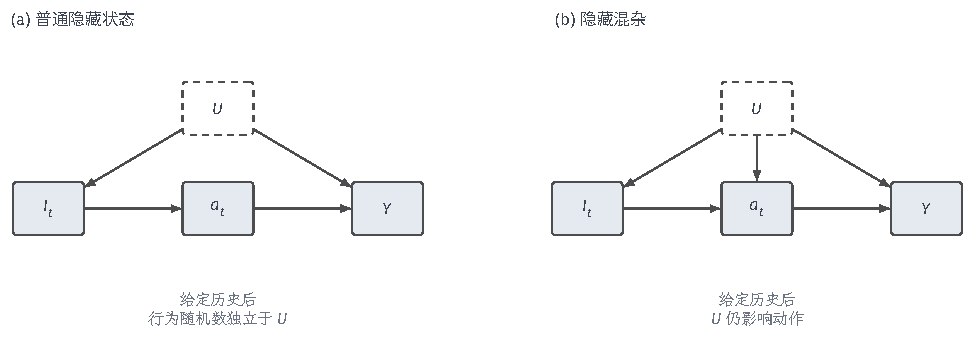
\includegraphics[width=163.714mm]{figures/10-reinforcement-learning/02-information-and-reward/tikz/rl-information-confounding.pdf}
  \caption{隐藏状态与隐藏混杂的区别。两图中的$U$均未记录，$I_t$为记录历史，$Y$为未来反馈。左图假设行为仅由$I_t$和独立随机数决定；右图多出$U\to a_t$，给定$I_t$仍不能阻断动作与后果之间的未记录共同原因。箭头表示因果假设。}
  \label{fig:rl-information-confounding}
\end{figure*}

有时可以用代理变量补充对隐藏量的间接观测，或增加传感器观测，但识别仍需明确的条件独立、可逆性或完备性等结构。字段变多不说明这些条件成立。部分POMDP离策略评价工作利用代理观测和矩阵秩条件处理隐藏机制，不能将这类结论改写为训练循环网络即可消除混杂\scite{rl4-tennenholtz2020-pomdp-ope}

% Outline: 4.6.3
\subsection{完全可识别时的历史表示与决策学习}
\label{sec:rl-information-full-identification}

先考虑不含上述隐藏混杂的一组条件：日志从回合开始完整保留$I_t$，行为以已知$\beta_t(a_t\mid I_t)$随机选择，给定历史后的随机数与潜在环境独立；目标也只使用记录历史，初始分布和环境共同，目标轨迹有行为支持。于是每个历史层内的动作按已知机制分配，物理状态隐藏不再给行为增加未知依据。我们可以据此计算目标与行为的可见回合记录比，获得点识别目标价值所需的校正。

隐藏状态本身并不阻止评价。仍用上面的$M_+$教学环境，若收集者不再按类型选动作，而是对每种类型都用独立公平随机数选$a_0$或$a_1$，两个动作组就都含有同样的总体类型混合。在总体上，$a_0$组奖励均值为$(1-1)/2=0$，$a_1$组为$(3+1)/2=2$，正好对应始终执行该动作的价值。状态类型仍不可见，改变的是动作组不再由类型挑选；正确随机化给出了将记录反馈用于目标行动的依据。

现在将第~\ref{sec:rl-information-estimators}~节的校正用于以可见历史为依据的策略。可见回合记录写成
\[
  \tau^o=(o_0,a_0,r_0,\ldots,o_H).
\]
给定历史和动作后的反馈分布记作$q(y_{t+1}\mid I_t,a_t)$。上述行为条件使目标与行为共享反馈因子。将轨迹密度按时间展开，再以目标密度除以行为密度，共同初始项和反馈项约去，得到
\begin{equation}
  \label{eq:rl-information-history-is}
  \frac{p_\pi(\tau^o)}{p_\beta(\tau^o)}
   =\frac{p(o_0)\prod_{t=0}^{H-1}
                  \pi_t(a_t\mid I_t)q(y_{t+1}\mid I_t,a_t)}
          {p(o_0)\prod_{t=0}^{H-1}
                  \beta_t(a_t\mid I_t)q(y_{t+1}\mid I_t,a_t)}
   =\prod_{t=0}^{H-1}\frac{\pi_t(a_t\mid I_t)}
                              {\beta_t(a_t\mid I_t)}.
\end{equation}
隐藏状态已在共同反馈因子中积分，因此最终只保留历史条件动作比。也可以先在完整隐藏轨迹上消去共同环境项，再求和隐藏状态；由于两策略的动作概率都只依赖可见历史，才能将它们提出该求和。

这一消去不能通过将$I_t$随意替换为$o_t$保留。行为若记住早期提示，只按当前画面拟合出的边缘频率就不是实际动作条件概率。专家若还看到例~\ref{ex:rl-information-confounding}~中的$U$，其动作项会随隐藏类型变化，无法从隐藏状态求和中提出，校正便失去依据。

识别条件成立后，可以直接按完整历史评价，或用有依据的充分表示降低计算成本。正确POMDP已知时用精确信念，预测结构可识别时可用PSR；潜在模型、循环或注意力记忆则需要检查允许动作上的预测或控制充分性。相应地，FQE可以在有限时域历史树上回归，行为约束作用于$\pi(a\mid I)$，提取动作时查询同一历史或经过论证的充分表示。直接保留历史减少了压缩假设，却可能使历史动作组合非常稀疏。

将完整历史换成$\bm z_t$，需要同时保留两种关系。一是目标策略和行为策略是否能从该表示确定实际动作概率，二是表示是否保留计算目标继续回报所需的历史差别。只证明网络能预测下一帧，不足以同时证明这两点；尤其不能把专家未记录的线索通过训练自动补进$\bm z_t$。识别是日志与生成条件提供的依据，表示是利用这些依据的计算选择。

这些计算仍有表示构造、行为概率估计、有限轨迹采样与优化误差，报告时应分开。训练用burn-in恢复记忆，部署却每$L$步清零，会变成不同策略；训练读到回合开始提示，部署只有窗口，也不是原来评价的对象。总体可识别排除了相同记录总体分布对应不同目标值的不唯一性，但在有限训练记录下，所选网络与优化程序仍未必给出准确估计。

早期提示任务可以将表示错误与不可识别分开。假设行为在每种提示下随机尝试两个出口，完整历史也被记录，则动作价值在总体上可识别。一个编码器保留$c$，另一个只重建走廊图像；延迟很长时，提示帧占平均重建损失的比例很小，两者重建误差可能相近。按原例不折扣成功奖励，前者仍可达到1，后者至多$1/2$。此时失败来自编码遗漏，不能解释为环境本来无法识别。

% Outline: 4.6.4
\subsection{部分可识别时的历史表示与决策学习}
\label{sec:rl-information-partial-identification}

若同一日志和结构仍容许多个价值，就需要保留定义~\ref{def:rl-information-identified-set}~中的一致模型集合$\mathcal M$，而不是选一个拟合模型当作唯一真相。对于固定$\pi$，比较$\mathcal M$内各模型的价值，取下确界和上确界，计算
$[\inf_MJ_M(\pi),\sup_MJ_M(\pi)]$，
作为识别集合的上下包络；也可改变允许的混杂强度，检查敏感性范围。包络只描述最小和最大边界，未必每个中间值都可实现。有限日志还须在外层加入总体分布未知的采样误差。

确定价值差的正负可能不必分别确定两个价值的数值。固定两个候选，在每个相同模型中先计算$\pi_1$价值减去$\pi_2$价值，再对$\mathcal M$取下确界。若这个最小边界仍为正，全部允许模型便给出同一排序；只看平均模型不够，因为另一个同样符合日志的模型仍可能反转次序。

\begin{example}[不知道共同偏移，仍知道谁更好]
  \label{ex:rl-information-partial-order}
  构造由$u\in[0,10]$参数化的一致模型，并令
  $J_u(\pi_1)=u+1$、$J_u(\pi_2)=u$。两个价值包络$[1,11]$与$[0,10]$大幅重叠，同一模型中的差却恒为1，因此$\pi_1$总较好。若将单独包络端点相减，$1-10=-9$对应为$\pi_1$取$u=0$、为$\pi_2$取$u=10$；这是松的包络差，不是任一共同模型的真实性能差。
\end{example}

\begin{theorem}[共同模型下的性能差确定排序]
  \label{thm:rl-information-partial-order}
  给定非空一致模型集合$\mathcal M$，在共同的任务、初始分布和时域口径下，假设两个固定候选策略在每个模型中的价值均为有限实数。若
  \[
    \inf_{M\in\mathcal M}
          [J_M(\pi_1)-J_M(\pi_2)]>0,
  \]
  则所有允许模型都给出$\pi_1$优于$\pi_2$的排序，两个单独价值区间即使重叠也不影响结论。
\end{theorem}

\begin{proof}
  将下确界记为$c>0$。定义保证任意同一个$M\in\mathcal M$均满足
  $J_M(\pi_1)-J_M(\pi_2)\geq c>0$，于是每个模型的排序相同。比较两策略时未切换模型，下确界也无须由某个模型取到，不等式仍成立。
\end{proof}

同一模型比较的要求与前面配对日志有相似的消差思路，但不确定性的来源不同。配对评价让两估计共用一条随机轨迹，可能消去采样波动；这里让两价值共用同一个尚未识别的环境，消去共同未知收益。增加独立日志可减小前者的波动，未必消除后者的模型歧义。两个单独区间因此不能不加判断地相减来替代共同模型差。

这里两候选共享未识别收益$u$，而“多得1”由额外结构假设给定，不能从拟合日志自行宣称。若允许策略只有$\pi_1,\pi_2$，为使选择在每个相容模型中都有依据，可以先各自对$u\in[0,10]$取最坏回报，再在两策略中最大化；最坏价值1和0会选中$\pi_1$。直接计算相对$\pi_2$的共同模型差下界则给出改进1。若另加不得偏离已覆盖历史的约束，且它排除了$\pi_1$的新历史，允许类只剩$\pi_2$，这项已由结构支持的改进也被放弃。保守限制可防止无依据推断，也可能因策略类过窄损失回报；系统的鲁棒优化见第~\ref{chap:rl-trustworthy}~章。

增加同类样本可以缩小采样误差，却不会自动排除总体上仍相容的模型。图~\ref{fig:rl-information-identification-width}~假设总体识别区间$[1,3]$，仅为示意将外层统计半径设为$2/\sqrt n$。样本增加时，外层范围缩到$[1,3]$而非单点。这是区分两种宽度的解析草图，不是算法经验曲线，也不是已经推导的置信保证。

\begin{figure}[htbp]
  \centering
  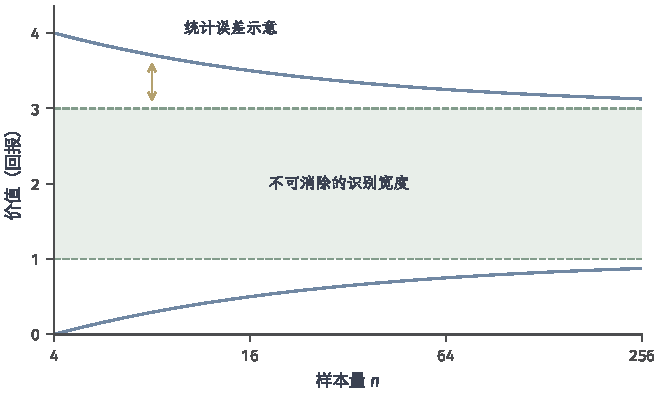
\includegraphics[width=112.000mm]{figures/10-reinforcement-learning/02-information-and-reward/matplotlib/rl-information-identification-width.pdf}
  \caption{教学识别区间$[1,3]$与示意外层范围$[1-2/\sqrt n,3+2/\sqrt n]$。实线范围随样本量缩小，虚线之间的非零宽度来自允许模型仍有差异；半径公式仅用于解释两种不确定性。}
  \label{fig:rl-information-identification-width}
\end{figure}

% Outline: 4.6.5
\subsection{不可识别时的学习边界与信息补充}
\label{sec:rl-information-unidentifiable}

若一致模型仍支持相反排序，当前目标决策就没有被识别。例~\ref{ex:rl-information-confounding}~的日志在两个模型下似然完全相同，最优动作却分别为$a_0$、$a_1$；缺口是专家选择所依据的未记录类型及其他动作的反事实后果。更细的当前观测编码不会补出未记录的类型及各类型下未尝试动作的后果，复杂模型收敛到任一解释也不能证明排序正确。

可以通过收缩目标或补充依据继续推进。缩小$\Pi$只比较日志支持的策略，或将全局最优改为基线附近的有限决策，改变的是要回答的问题。增加已知动力学、行为随机化或代理观测等可核验假设，改变的是允许模型集合。新假设须有外部依据才能排除相容解释，方便拟合的设定不能冒充原日志中的事实。

\begin{table*}[htbp]
  \centering
  \small
  \begin{tabularx}{\linewidth}{p{26mm}XX}
    \toprule
    缺失的记录或模型约束 & 可补采字段或补加假设 & 仍须核验的条件 \\
    \midrule
    较早提示未记录 & 从真实回合开始的长历史或足够记忆摘要 & 提示是否确实保留；部署可用性与回合边界一致 \\
    行为机制不明 & 当时动作概率、策略版本及相关上下文 & 动作概率所依据的历史字段完整且正确；潜在类型上的支持仍可能缺失 \\
    当前状态混叠 & 新传感器、主动辨识动作或代理变量 & 新观测能否区分与控制有关的状态；代理识别条件 \\
    目标行为无覆盖 & 受控随机交互、指定区域的实验 & 查询确实覆盖目标历史动作；代价和安全权限允许 \\
    初始或任务条件不明 & 初始状态、目标及采样分层元数据 & 评价分布与部署分布一致，或有正确校正 \\
    \bottomrule
  \end{tabularx}
  \caption{补采字段与补充假设要对应具体缺口。记录隐藏类型可以消除部分混杂，却未必补齐每种类型下未尝试的动作；新增字段与新增行为各有不同作用。}
  \label{tab:rl-information-information-repair}
\end{table*}

表~\ref{tab:rl-information-information-repair}~逐项对应了可补采的日志字段或补加的结构假设。单独补记概率未必够：例~\ref{ex:rl-information-confounding}~中专家在每种类型上都确定性行动，即使记录$U$，该类型的另一动作仍无支持。识别固定策略价值，还需在允许类型内受控随机行动，或有依据的跨类型、跨动作结构。更长的同类日志不能替代这些行为概率字段或模型结构假设。

若允许有限交互，可以分别安排状态辨识与策略验证预算。辨识选择能区分相容模型的传感或动作，并在需要时更新表示；验证则固定新策略、其可读取的历史及记忆初始化协议，取得独立的策略回报证据。自适应辨识取得的记录不能未经处理便当作独立最终测试。权限不足，或新反馈仍在相容环境中同分布时，无法判断的结论应保留。网络容量可帮助降低表示或拟合误差，却不能仅凭同分布的可见记录辨清本来不可区分的环境。

% Outline: 4.7
\section{本章小结}
\label{sec:rl-information-summary}

章首的小车问题现在可以分别回答。速度不可见时，需要由历史保留线索，或用信念与记忆形成决策依据；缺少左转经验时，需要检查收集机制与覆盖，判断左转后果能否从日志确定。Tiger说明模型已知仍可能值得付费辨认当前状态，未覆盖动作反例则说明状态完全可见也仍可能无法识别价值。仅增加记忆不能补齐动作后果，仅补充同类行为也不能找回未记录的线索。

排除了同样日志对应不同答案的歧义以后，还需要用有限记录计算价值；这一步会有样本波动、行为概率误差和模型误差。再用估计值改策略时，策略可能主动寻找高估动作，因此还要检查估计是否覆盖新的选择。行为约束限制策略偏离日志记录中的行为，悲观目标扣除未证实的收益，二者都需要自己的误差依据。最后评价的对象是实际提取出的执行策略，不能用价值网络的训练损失或模型内回报替代它。答案能够确定、数值能够估计、目标能够优化和策略能够验证，分别跨过了不同的障碍。

两类限制叠加时，执行历史、日志字段和收集者选动作的依据要共同核对。在完整历史、共同环境与初始条件、正确随机化机制和目标支持下，隐藏状态可从共同反馈项中积分，概率比只含历史条件动作概率。存在未记录行为依据时，相同日志却可能对应相反排序。部分识别仍可能通过共同模型差作出有限决策，排序不可识别时则需收缩结论或补采能区分候选模型的反馈或补加有依据的结构约束。随策略结论报告执行策略可读历史、日志机制、覆盖范围、表示假设、查询预算及误差依据，才能确定它适用于哪里。

\chapter{奖励受限下的强化学习}
\label{chap:rl-reward}

一台配送机器人已经学会移动和避障，但这只解决了“能做什么动作”；我们还必须告诉它“什么样才算一次好的配送”。前几章默认环境每步都会返回一个可信的数值奖励，本章要处理的正是这个奖励本身出问题的情形。请人示范路线可以提供可用动作，但示范者选择电梯，可能为了更快，也可能为了省电或保持包裹水平——单凭动作记录，背后的计分标准未必已经确定，还需要进一步判断这些记录究竟支持哪一种目标解释。

即使已经明确约定“正确签收且包裹完好”、也能拿到可靠的总分，学习仍有困难：终局失败只告诉我们这次配送坏了，却没有直接标出是核对、装载还是搬运哪一步出的错，需要想办法把最终结果联系回早期决策。反过来，如果贪图反馈及时，改成每移动一米就给分，反馈倒是又快又密，机器人却可能靠不停地绕路刷高分、根本不去交付——这是数值标准本身定错了，靠增加反馈或加快传播都无法补救。因此，反馈“表达了什么”“能否说明每一步的局部贡献”“是否真的符合我们想要的行为”，是三个必须分别解决的问题。

第~\ref{chap:rl-learning}章虽然不知道期望奖励是多少，但仍假定每次交互后都能读到一个奖励样本；第~\ref{chap:rl-information}章则检查能看到哪些观测、历史记录是否完整，以及日志的状态动作覆盖是否足以支持决策。本章保留前两章的全部学习工具，只改变喂给它们的反馈。我们要分别判断三件事：当根本没有可信的标量奖励时，示范、偏好、检查等其他记录能约束哪些行为目标；当只有一条轨迹的总分时，怎样用它更新中途的局部决策；当训练分数确实提高时，实际行为是否真的满足了最初的要求。图~\ref{fig:rl-reward-map}说明这三个问题如何共同支撑反馈学习。它们是可以叠加的限制，而不是必须排队依次排除的三种故障。

\begin{figure*}[htbp]
  \centering
  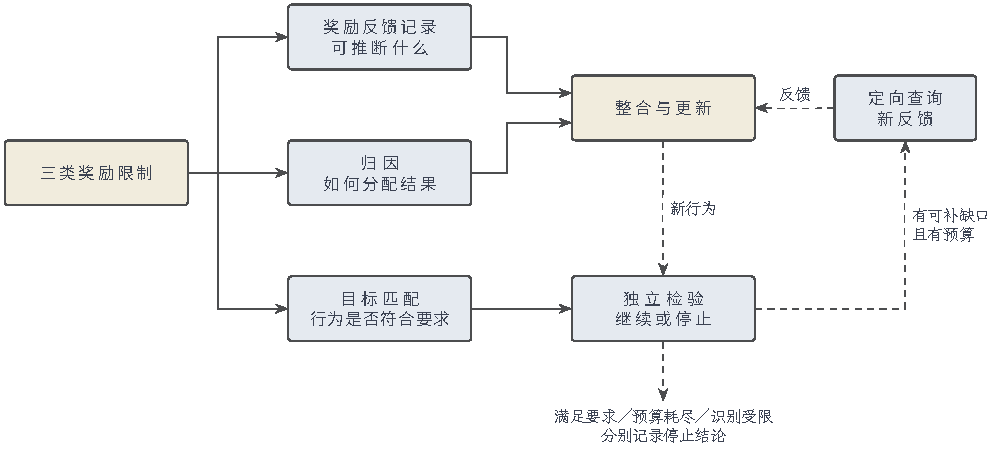
\includegraphics[width=169.000mm]{figures/10-reinforcement-learning/02-information-and-reward/tikz/rl-reward-map.pdf}
  \caption{三类奖励限制与反馈学习的关系。实线表示观测、归因和目标匹配分别为反馈整合、策略更新及行为检验提供依据，不规定三者的解决顺序；虚线表示取得新行为和新反馈后进入下一轮。停止可能因为证据已满足要求，也可能因为预算耗尽或区分候选奖励所需的反馈无法取得，三者支持的结论不同。}
  \label{fig:rl-reward-map}
\end{figure*}

本章仍用$r_t$表示执行$a_t$后的奖励，用$J(\pi)$表示未归一化的期望折扣回报。为观察反馈落在哪个环节，我们另设一个四步配送任务：机器人依次核对包裹、装载、搬运和交付，状态包含包裹身份、位置及完好情况。这个案例不沿用前文随机网格的精确动力学；除特别说明外，反馈在交付后才给出。本章用于计算的人工数字都是教学假设。

% Outline: 5.1
\section{奖励信号的三类限制}
\label{sec:rl-reward-limits}

% Outline: 5.1.1
\subsection{奖励观测受限}
\label{sec:rl-reward-observation}

机器人不知道一条路线的平均耗电量时，仍可在每次执行后读电表、再用样本均值估计期望耗电。若固定路线、负载及其他运行条件，独立重复执行，且耗电量的期望有限，就可以用可信的电表读数估计同一条件下的期望耗电；有限次执行仍有抽样误差。这仍是第~\ref{chap:rl-learning}章讨论过的未知奖励期望估计。但若目标改为“把包裹妥善交给收件人”，而日志里只记录了移动距离，问题的性质就变了：距离既没说明交给了谁，也没说明包裹有没有破损。此时缺少的是能够表达目标的观测，而不是均值估得不够精确——收集再多的距离记录，也判断不了交付质量。

同一次配送其实可以留下多种不同记录：专家当时怎样装载（示范了一个动作）、收件人给这次配送打几分（一个评分）、两条路线哪条更合意（一次比较）、包裹编号是否通过核对（一次检查）。它们绝不是四种等价的“正确标签”：动作记录描述已经发生的行为，评分给出某个尺度上的数值，比较只给相对先后，检查则只判断某个指定条件成不成立。因此必须先说清每条记录评价的对象，才能决定它应该进入动作拟合、奖励学习还是条件验证。

\begin{definition}[替代反馈的形式与粒度]
  \label{def:rl-reward-feedback}
  \term{示范}（demonstration）记录决策者实际采取的行为，可以是某状态上的动作，也可以是整条轨迹。\term{评分}（rating）按照约定尺度给被评价对象一个数值。\term{偏好}（preference）记录在相同比较条件下，评价者如何排列两个或多个对象。\term{验证反馈}（verification feedback）判断对象是否满足指定条件，并可附带检查证据。反馈的\term{粒度}（granularity）是这次判断实际评价的单位，可以是动作、步骤、轨迹片段或完整轨迹。记录到达的时间不必等于被评价动作发生的时间。
\end{definition}

粒度和到达时间是两回事，不能混为一谈。签收之后才补记一条“装载时身份错误”，它评价的仍是装载那一步，只是这条记录到达得晚；而“这次配送 0 分”评价的是整条轨迹，并不等于给每一步都打上了 0 分的标签。把一个轨迹总分送进各步的策略更新，本质上是在用总结果去估计各动作的影响（这是下一节奖励归因要处理的事），并没有自动把评价对象细化到每一步。

这四种记录描述的行为和评价内容各不相同。示范只告诉我们“当时做了什么”，对没有选择的动作毫无评价；带等距尺度的标量评分还能表达评价之间的差距，但若分数只是有序等级（比如一星到五星只表示好坏次序），数字之差就不再自动对应评价之差——把等级用于期望回报前，必须显式规定等级到训练效用的编码方式。偏好可以只给顺序而不给绝对分数；验证器的“通过”标记则只支持被检查的那一个条件。表~\ref{tab:rl-reward-forms}还单列了查询权限：读取已有的示范记录，与获准继续向专家追问，是两种不同的访问能力，前者不能代替后者。

\begin{example}[等级排序没有确定期望效用]
  \label{ex:rl-reward-ordinal-score}
  策略甲各以$1/2$概率得到1星和5星，策略乙总得4星。直接按星数计分时，甲的期望分为3，乙为4。若星级只表达次序，将1、4、5星分别编码为0、1、100仍保留这些等级的排序，此时甲的期望为50，乙为1，比较结果反转。因此，等级次序本身没有确定怎样比较这两种随机结果；按平均星数优化，可以作为任务方明确选择的训练目标约定。
\end{example}

\begin{table*}[htbp]
  \centering\small
  \begin{tabularx}{\linewidth}{@{}>{\raggedright\arraybackslash}p{17mm}*{5}{>{\raggedright\arraybackslash}X}@{}}
    \toprule
    形式 & 反馈对象 & 粒度 & 噪声来源 & 查询权限 & 可推断对象 \\
    \midrule
    示范 & 已执行动作与上下文 & 动作、轨迹 & 次优专家、漏记任务指令或专家当时可见的状态 & 固定日志或另行授权的专家查询 & 行为条件分布；附加理性假设下的奖励约束 \\
    评分 & 单个被评价行为 & 步骤、片段、轨迹 & 尺度漂移、反应延迟 & 可只提供历史评分 & 该尺度下的评价函数 \\
    偏好 & 同条件候选行为 & 一对片段或轨迹 & 次序效应、偏好异质性 & 固定比较或主动选对 & 比较概率、相对效用 \\
    验证 & 产物或状态关系 & 步骤、结果 & 规则遗漏、执行误差、误判 & 可离线复查或在线调用 & 指定条件的通过情况 \\
    \bottomrule
  \end{tabularx}
  \caption{四种反馈形式及其记录对象。形式说明记录表达什么，查询权限说明还能补充什么。人类、AI、规则和执行器描述反馈来源，同一来源可以产生多种形式。}
  \label{tab:rl-reward-forms}
\end{table*}

例如，人和模型都可以提供示范、评分或成对偏好。身份核对规则可以返回通过标记，实际执行开箱操作的检查器也可以返回破损结果。这里“人类反馈”回答谁在判断，“偏好反馈”回答判断怎样记录，两者可以同时描述同一条记录，不是互斥类别。

% Outline: 5.1.2
\subsection{奖励归因受限}
\label{sec:rl-reward-credit-limit}

假设日志已经准确记下“包裹完好、交付成功”，我们仍然不知道这份成功里哪些先前决策值得强化：核对身份、平稳搬运、甚至选了一条容易的路线，都可能与成功同时出现。\term{奖励归因}（reward credit assignment）要做的，就是把长期结果联系回此前的具体决策，为每一步的局部更新提供“贡献”判断。第~\ref{chap:rl-learning}章已经用回报、TD 误差和优势估计来传播结果；本节则要进一步检查这些工具实际读到了哪些结果评分和过程标签，以及还有哪些贡献始终没有被观测到。

四步配送如果只在最后才得到成功分，那么前三步即时奖励为 0，但这个 0 既不表示它们没有贡献，也不表示检查器判定它们出错——它只说明当前的计分规则还没有给出对早期步骤的局部评价。要更新早期动作有两条不同的路子：一是把终局结果沿动作概率的梯度回传（传播已有结果），二是补充新的过程检查（取得新的评价证据）。

\begin{table*}[htbp]
  \centering\small
  \begin{tabularx}{\linewidth}{@{}>{\raggedright\arraybackslash}p{27mm}*{3}{>{\raggedright\arraybackslash}X}@{}}
    \toprule
    现象 & 缺口 & 主要影响 & 不能直接推出什么 \\
    \midrule
    非零奖励很少 & 多数尝试没有区分信号 & 难以探索到成功轨迹 & 一旦成功就能正确归因 \\
    反馈延迟长 & 行动与反馈相隔许多步 & 贡献需跨步传播；随机轨迹下估计可能更难 & 回报方差必然增大或反馈语义错误 \\
    只有轨迹总分 & 局部贡献未被观测 & 无关动作也可能分享相同结果 & 每一步都有独立监督 \\
    反馈噪声大 & 相同行为的判断不稳定 & 估计方差和误排序增加 & 噪声一定来自时间延迟 \\
    \bottomrule
  \end{tabularx}
  \caption{影响奖励归因的四种反馈性质。非零奖励少、反馈来得晚、只评价整条轨迹及判断有噪声，可以在同一任务中同时出现，但各自造成的缺口不同。}
  \label{tab:rl-reward-credit-limits}
\end{table*}

反馈到达得晚，不等于回报方差必然增大。确定性终局得分无论晚到多少步，方差仍为零。若固定策略和随机得分$X$的分布，只把奖励发生时刻从0移到$h$，在固定$\gamma<1$下，折扣回报的方差为$\gamma^{2h}\operatorname{Var}(X)$，反而不大于原方差。较长交互中，随机状态、动作及评分噪声可能使局部贡献更难估计；判断方差怎样变化时，必须固定所比较的估计量及其他条件。若只是记录晚到、奖励所属时刻不变，离线计算的回报也不会因此改变。

按照表~\ref{tab:rl-reward-credit-limits}，我们可以先区分尚未找到成功行为与已经找到成功行为却不清楚贡献这两种情况。机器人始终找不到收件人时，增加探索或提供成功示范可能补上行为线索。若日志中已有许多成功配送，但身份核对总与无关的扫码动画一起出现，就需要辨认哪一个动作影响结果。重复收集相同组合未必能区分二者；给每次动画播放加分虽然增加了反馈频率，也没有提供能区分各动作贡献的评价依据。

% Outline: 5.1.3
\subsection{奖励与行为目标不匹配}
\label{sec:rl-reward-mismatch-limit}

若计分规则是“每移动一米得一分”，机器人就能靠不断绕圈把回报刷得很高，却始终不完成配送。这里要特别注意：优化器并没有失灵，它正忠实地最大化给定分数；出问题的是数值标准本身没有表达交付要求。要诊断这种偏差，必须把两件事分开——我们真正希望发生的行为，与训练实际在优化的数值。

\begin{definition}[奖励、回报、效用与行为要求]
  \label{def:rl-reward-objective}
  单步奖励$r_t$是交互协议返回的标量，累计回报$G_0=\sum_t\gamma^t r_t$按约定的时间权重汇总这些标量。\term{效用}（utility）表示决策者如何评价结果或结果分布，可记为$u(\tau)$或策略评价泛函$\mathcal U(\pi)$，不预设它等于$J(\pi)$。\term{行为要求}（behavioral requirement）规定希望发生什么以及在什么条件下发生，例如交给正确收件人、保持包裹完好并满足能耗要求。\term{代理奖励}（proxy reward）是训练所用的数值编码；它是否表达了这些要求，须用独立证据检验。
\end{definition}

据此再看三种限制：里程计分即使即时且准确，也可能遗漏任务目标；“正确收件人且完好”的终局标记可以表达明确的成功条件，但早期动作要经过多步才得到反馈。有效路线示范能够帮助行动，却未必确定各项奖励权重。同一任务还可以同时具备三种限制，例如示范不记录破损、评分延迟到终局，训练又额外奖励里程。

选择学习办法要先定位缺口。缺少可靠信号时需要补充能表达目标要求的示范、评分、偏好或验证结果，缺少局部贡献时需要检查结果怎样进入更新，标准遗漏要求时则需要修订目标。训练损失下降只能说明模型更符合所选训练准则，不能同时证明反馈覆盖充分、归因正确和编码完整。交付身份、完好情况及能耗的独立检查应在优化前约定；若事后随行为改变标准，就失去了判定偏差的共同依据。这一判断以配送要求、可接受行动及评价条件已经约定为前提：代理分数只是要求的数值表达，目标是否达成仍需对相应行为和结果取证。目标、训练信号与行为边界的区分可参考\BookChapterRef{chap:trust-alignment}{卷3《基础、理论与可信性》中讨论目标对齐与行为约束的章节}。

% Outline: 5.2
\section{奖励观测受限下的强化学习}
\label{sec:rl-reward-alternative}

假设配送日志拿不到可靠的逐步奖励，但保留了专家路线、两条路线的比较或签收检查结果。这时可以走三条不依赖唯一奖励的路子：直接用动作示范拟合策略、用偏好约束效用的相对大小、或用验证结果构造策略更新信号，而不必先反推出一个唯一的数值奖励。每种反馈究竟能约束什么，完全取决于记录实际表达的内容以及它在什么假设下产生。

% Outline: 5.2.1
\subsection{替代反馈与可推断对象}
\label{sec:rl-reward-inference}

在同一个配送任务中，示范可以记录专家选择电梯，偏好可以记录收件人更喜欢平稳但较慢的配送，身份验证则只检查是否交给正确的人。选择电梯没有单独说明“慢一些更好”，身份通过也没有证明包裹无破损。若把这些记录统一改成“正例”，我们就无法再分清它们支持哪种结论、排除了哪种目标解释。

当状态在示范与部署时都可读取、且两者使用相同状态字段时，策略$\pi(a\mid s)$给出某状态上的动作分布，占用度量$d^\pi(s,a)$汇总长期访问状态和动作的概率；价值$V^\pi,Q^\pi$预测给定奖励和策略下的后续回报。奖励$R(s,a)$规定单步期望计分，效用表达评价者怎样看待结果。状态不可见时，执行策略只能以部署可得历史$I_t$为依据，不能把训练日志中的特权状态直接作为部署时可读取的决策依据。这些对象相互联系，但一条记录对其中一个对象施加约束，并不自动唯一确定其他对象。表~\ref{tab:rl-reward-inference}列出各类记录可以支持的学习对象。

\begin{table*}[htbp]
  \centering\small
  \begin{tabularx}{\linewidth}{@{}>{\raggedright\arraybackslash}p{22mm}*{4}{>{\raggedright\arraybackslash}X}@{}}
    \toprule
    反馈 & 候选推断对象 & 额外假设 & 训练交互 & 拟合所得对象 \\
    \midrule
    状态动作示范 & 策略 & 记录的状态或可得历史足以确定专家的条件动作分布，覆盖可用 & 行为克隆不需要 & 动作分布 \\
    专家与策略轨迹 & 占用、软价值 & 共同环境，轨迹采样口径一致 & 占用匹配通常需要 & 策略或价值函数 \\
    专家轨迹 & 奖励、特征期望 & 专家理性、奖励函数类、动态模型 & 需规划或采样权限 & 奖励候选及策略 \\
    标量评分 & 评价函数 & 尺度、对象与时间归属明确 & 拟合本身不需要 & 评分预测器 \\
    成对偏好 & 效用差、策略 & 比较模型与共同条件 & 拟合可离线；在线RL另需新采样 & 奖励模型或偏好策略 \\
    过程、结果验证 & 条件通过概率 & 规则有效、检查前提满足 & 在线更新需可调用验证 & 验证信号与策略 \\
    \bottomrule
  \end{tabularx}
  \caption{不同记录可支持的推断、假设及所得模型或策略。同一反馈可以用于多个学习对象，同一对象也可以结合多种反馈。“不需要交互”只说明拟合阶段的访问要求，不表示固定示范记录已覆盖新策略将访问的状态和动作。}
  \label{tab:rl-reward-inference}
\end{table*}

一个单步例子即可看出不唯一性。任务只有左、右两个动作，专家总选左；奖励$(R(\text{左}),R(\text{右}))=(1,0)$和$(10,9)$都能使左最优。若记录只保留甲、乙、丙的确定排序，效用$(3,2,1)$和$(100,2,0)$也都给出甲优于乙、乙优于丙，但它们的效用差不同，未必在同一个随机偏好模型中产生相同比较概率。排序只给出先后次序，完整比较概率还给出选择频率；即使概率已知，共同加法常数等歧义通常仍然存在。

新增查询能否解除歧义，取决于它提出了什么新问题。若允许主动查询，我们可以比较此前未比较的路线，或询问专家在当前策略偏离后怎样恢复。按同一采集或评价协议取得新的独立记录，并满足相应矩条件时，可以提高已涉及行为的估计精度；仅重复使用已有记录不会增加这类统计证据，也不会补出从未涉及的要求。能识别的是动作、排序还是奖励，仍须按记录内容及生成假设分别判断。

% Outline: 5.2.2
\subsection{从示范直接学习策略}
\label{sec:rl-reward-bc-dagger}

专家既然已经给出了可用动作，最直接的想法就是让自己的策略在相似状态、或在部署时能读到的相同历史下复现这些动作。前一章把“拟合日志里实际采取的动作”称为\term{行为克隆}（behavioral cloning, BC）；在这里，它把示范记录中的状态（或可得历史）当作条件变量，把专家动作当作监督标签，本质上是一个监督学习问题。要衡量一个离散动作策略复现示范的程度，可以惩罚它给专家动作分配的概率太小。设任务有$t=0,\ldots,H-1$共$H$步，专家在各时刻访问状态的分布为$\nu_t^{\mathrm E}$；对这些状态以及专家在其中选择的动作取期望，再对时间平均，得到总体负对数似然
\begin{equation}
  L_{\mathrm{BC}}(\bm{\theta})
  =-\frac1H\sum_{t=0}^{H-1}
  \mathbb E_{\substack{s\sim\nu_t^{\mathrm E}\\
              a\sim\pi_{\mathrm E}(\cdot\mid s)}}
       \log\pi_{\bm{\theta}}(a\mid s).
  \label{eq:rl-reward-bc}
\end{equation}
最小化该损失，就是在专家访问分布上最大化示范动作的平均对数概率，并不要求每条记录的概率都同时增加。训练时用专家示范训练样本$D_{\mathrm E}$的平均负对数似然估计这个期望，其中$D_{\mathrm E}$是按声明采集机制取得的有限示范记录组；候选策略类给出允许的条件动作分布，学习规则还要规定目标构造、初始化、更新、停止与策略读出。训练拟合与独立评价使用不同职责的样本，不能仅凭训练动作似然较高断言部署回报改善。一次参数更新可写为
$\bm{\theta}^{(k+1)}=\bm{\theta}^{(k)}
-\eta\nabla_{\bm{\theta}}\widehat L_{\mathrm{BC}}$，
完成一次参数拟合，其中$\eta$为步长。这些示范记录由专家产生，不是当前策略执行得到的；每次遍历都要为记录计算策略概率和梯度，但不需要奖励标签或重新运行环境。

连续动作还可以用平方误差$\mathbb E\lVert f_{\bm\theta}(s)-a\rVert_2^2$拟合动作数值；在无限容量下，最小化这个误差得到的是条件均值。但均值动作未必能用。设想专家绕障时等概率选择$-1$和$1$（左绕或右绕），两者都是有效路线，可它们的均值$0$却可能让机器人直冲障碍。要保留示范中的多种可行动作模式，就得显式表示一个多模态的动作分布，而不能只输出平均动作。均值出错还可能有另一个原因：日志漏记了任务指令，导致相同观测其实对应不同的专家动作；这种情况下单纯加大网络也无法恢复未记录的指令。

即使动作在专家示范覆盖的状态上拟合得很准，也不能保证策略实际运行时同样准。这里存在一个被称为“复合误差”的现象：专家几乎不会走进错误走廊，因此示范里没有那些状态；而克隆策略只要偶发走错一步，就会落入示范从未覆盖的状态，此后只能在陌生状态上继续决策、往往又走错，错误于是一层层累积。为看清早期错误为何代价更大，下面在共同环境中比较专家与学习策略，用“第一次与专家分歧”的概率给出一个保守上界。

先看$H=4$的尺度。若在第一步选错走廊，后面四步都可能付额外成本；若直到最后一步才与专家不同，只剩一步可能受影响。将每个可能分歧位置的最坏后果分别累计，出现$4+3+2+1=10$这个系数。若每个专家状态分布上的分歧概率至多$0.05$，相应保守成本差界为$0.5$。这不是每次错误都实际损失余下全部成本，而是用单步成本上限控制最不利情况；下面正式说明概率条件。

\begin{theorem}[行为克隆的首次分歧界]
  \label{thm:rl-reward-bc}
  给定正整数$H$和$\varepsilon\geq0$。考虑共同非空有限状态集、各状态非空有限合法动作集、共同初始分布与共同转移核的$H$步任务，每步成本$c_t(s,a)\in[0,1]$，总成本记为
  $C_H(\pi)=\mathbb E_\pi\sum_{t=0}^{H-1}c_t(s_t,a_t)$。
  专家动作映射为$g_{\mathrm E}$，其诱导策略为$\pi_{\mathrm E}(\cdot\mid s)=\delta_{g_{\mathrm E}(s)}$；记该策略在时刻$t$的状态分布为$\nu_t^{\mathrm E}$。若合法Markov学习策略$\pi$在每个专家状态分布上均满足
  \[
    \mathbb E_{s\sim\nu_t^{\mathrm E}}
    \bigl[1-\pi(g_{\mathrm E}(s)\mid s)\bigr]\leq\varepsilon,
  \]
  则
  \[
    C_H(\pi)-C_H(\pi_{\mathrm E})
    \leq \frac{H(H+1)}2\varepsilon.
  \]
  非平稳专家可把时间加入状态，结论不变。
\end{theorem}

\begin{proof}
  将两条轨迹放在同一概率空间中，使它们从相同状态出发，并在尚未出现动作分歧时共用环境转移的随机性。另在完整专家轨迹的每个$s_t^{\mathrm E}$上，抽取服从$\pi(\cdot\mid s_t^{\mathrm E})$的候选动作。令$B_t$表示该候选动作不同于专家动作；定理假设给出$\mathbb P(B_t)\leq\varepsilon$。

  首次分歧以前，两条轨迹的状态、动作和成本相同，所以截至$t$已发生分歧，只可能是在某个$j\leq t$出现了$B_j$。这个事件包含于$\bigcup_{j=0}^{t}B_j$，由并集界，其概率不超过$(t+1)\varepsilon$。分歧后两条轨迹可以任意发展，但单步成本均在$[0,1]$内，额外成本至多为1；未分歧时额外成本为0。对这一指示变量上界取期望，再按时间求和，
  \[
    C_H(\pi)-C_H(\pi_{\mathrm E})
    \leq\sum_{t=0}^{H-1}(t+1)\varepsilon
    =\frac{H(H+1)}2\varepsilon.
  \]
  并集界使用的是完整专家轨迹上的事件概率，并未假定“此前尚未分歧”条件下的错误率也等于$\varepsilon$，因此没有额外引入条件分布假设。
\end{proof}

由于每步成本至多为1，总成本差本身还不超过$H$，可以将界的右端取为$H$与上述二次项中的较小值。二次项来自一次早期分歧可能影响余下多步的估计，不是所有任务都会二次恶化的断言；若机器人能迅速恢复，实际额外成本可以小得多。

复合误差的根源是专家轨迹与学习策略执行轨迹所访问的环境状态分布不一致。一个自然的补救办法，是让专家专门对学习策略实际误入的状态补动作标签。\term{数据集聚合}（Dataset Aggregation, DAgger）反复执行当前策略、就它访问到的状态向专家查询，再把新标签对应的状态动作记录追加到训练样本中重新拟合。它改变的是交互训练记录的状态覆盖范围，使偏离后的状态也进入下一轮训练，而不是只在专家原有轨迹附近打转。图~\ref{fig:rl-reward-dagger}分别画出执行、查询和聚合三步；Ross 等给出了这一归约及其在线学习分析\scite{ross2011}。

\begin{algorithm}[一轮DAgger更新]
  \label{alg:rl-reward-dagger}
  \begin{algorithmic}[1]
    \Require 已聚合训练记录$D^{(k)}$，策略$\pi^{(k)}$，专家查询接口，轨迹预算$m$
    \Ensure 新增训练记录$D^{(k+1)}$与候选策略$\pi^{(k+1)}$
    \State 在获准环境中执行$m$条$\pi^{(k)}$轨迹，记录实际访问的状态
    \State 对这些状态查询$a_{\mathrm E}=g_{\mathrm E}(s)$，保留失败及偏离后的状态
    \State 将新标注记录$(s,a_{\mathrm E})$追加到$D^{(k)}$，保留重复记录，得到$D^{(k+1)}$
    \State 在聚合训练记录上最小化模仿损失，得到$\pi^{(k+1)}$
    \State 在独立轨迹上评价任务表现，并记录查询数与执行风险
  \end{algorithmic}
\end{algorithm}

\begin{figure}[htbp]
  \centering
  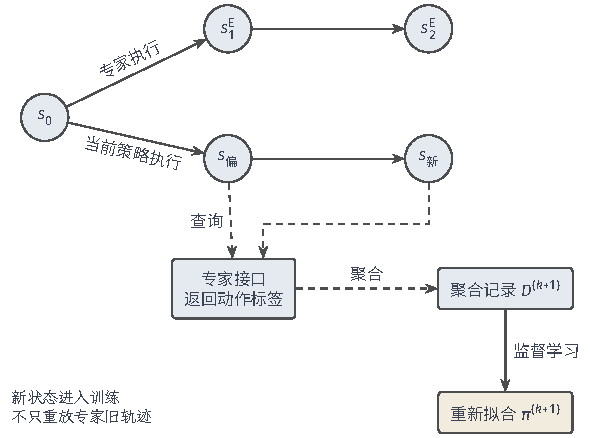
\includegraphics[width=99.977mm]{figures/10-reinforcement-learning/02-information-and-reward/tikz/rl-reward-dagger.pdf}
  \caption{DAgger补充当前策略偏离后的状态。两条轨迹从同一起点出发，分歧后对当前策略访问的新状态查询专家；新标签随追加后的状态动作训练记录进入下一轮。查询只取得动作标签，不表示专家已在环境中执行该动作。}
  \label{fig:rl-reward-dagger}
\end{figure}

例如，当前策略误入$s_{\text{偏}}$，专家标注“返回”。在二动作策略中，用logit $z$表示返回的对数几率，返回概率为$\sigma(z)$，其中$\sigma(z)=(1+\exp(-z))^{-1}$将实数转换为概率。若当前$z=0$，该标签的负对数似然梯度是$\sigma(0)-1=-1/2$；以$0.2$为步长下降，得到$z=0.1$，返回概率由$0.5$升至约$0.525$。这次更新利用了原专家示范未覆盖的错误状态。取得这些标签也有成本：每轮执行$m$条$H$步轨迹需要$mH$个环境步、至多$mH$次查询，并要重新拟合不断追加的训练记录组。

能否持续改善自身访问分布上的模仿损失，可以用在线学习的遗憾来描述：每轮损失在该轮策略访问分布上计算，比较基准则是预先指定策略类$\Pi$中，同一策略在全部轮次上的平均损失。若这些总体损失可直接获得，平均遗憾小意味着迭代策略的平均损失接近类内最小值，因而至少有一轮不超过该平均上界。

\begin{theorem}[理想化DAgger的无遗憾归约]
  \label{thm:rl-reward-dagger}
  固定正整数$H,K$、共同环境中的非空候选策略类$\Pi$，以及非负可测的模仿损失$\ell:\Pi\times S\to[0,\infty)$；假设下面各项期望均为有限实数，并给定有限常数$\varepsilon_{\mathrm{reg}}$。令$\nu_t^{\pi^{(k)}}$为第$k$轮策略在时刻$t$的状态分布，
  $\bar\nu^{(k)}=H^{-1}\sum_{t=0}^{H-1}\nu_t^{\pi^{(k)}}$，并定义
  $\ell_k(\pi)=\mathbb E_{s\sim\bar\nu^{(k)}}\ell(\pi;s)$。若$K$轮在线拟合满足
  \[
    \frac1K\sum_{k=1}^K\ell_k(\pi^{(k)})
    -\inf_{\pi\in\Pi}\frac1K\sum_{k=1}^K\ell_k(\pi)
    \leq\varepsilon_{\mathrm{reg}},
  \]
  则至少一轮$k$满足
  \[
    \ell_k(\pi^{(k)})
    \leq\inf_{\pi\in\Pi}\frac1K\sum_{j=1}^K\ell_j(\pi)
        +\varepsilon_{\mathrm{reg}}.
  \]
\end{theorem}

将遗憾不等式中的比较项移到右侧，就得到各轮自身分布损失的平均上界。再在实际生成的$K$个策略中取损失最小的一轮，利用
\[
  \min_k\ell_k(\pi^{(k)})
  \leq\frac1K\sum_k\ell_k(\pi^{(k)}).
\]
即可得到定理的结论。比较策略在所有轮次的分布上评价，分布本身不必相同。这个结果首先约束模仿损失；使用有限样本还要加入估计误差，混合执行专家时还要控制混合分布与自身分布的差异。若进一步推成任务成本界，需要模仿损失能控制动作错误，并且一次错误后专家恢复的额外成本有统一上界。平均遗憾条件本身不足以保证任意实现都具有线性时域成本界。实现时可以保存各轮候选，并按预先分配的预算，用独立验证回合比较它们；若选择依据是各候选自身访问分布上的模仿损失，还需为这些状态取得专家动作标签。验证误差须对参与选择的候选共同受控，选定后再用未参与选择的测试回合报告表现。若按任务回报选择，应另报告该指标的评价依据，不能把模仿损失的存在性结论直接当作任务回报保证。

动作模仿得像，不等于动作的后果代价相同。机器人“走错一条可以立刻返回的支路”和“把包裹交给错误的收件人”，在动作标签上都可能被记为与专家不符，但前者只多走几步、可以轻易挽回，后者却可能无法撤回。要在这两种错误之间合理地分配更新，光知道专家的正确动作还不够，还必须知道候选动作之后的长期代价。仅有动作标签时，DAgger 无法区分两种错误动作的后续代价；于是需要代价敏感的模仿或后续价值查询。\term{基于搜索的结构化预测}（search-based structured prediction, SEARN）将序贯预测转为代价敏感学习，通常通过后续执行估计各动作的代价；其中SEARN是方法专名，不是该英文名称逐词首字母的缩写。\term{聚合价值模仿}（Aggregate Values to Imitate, AggreVaTe）则聚合当前访问状态上的专家后续成本，使“动作不同但成本接近”也能进入比较。与仅查询专家动作相比，这些方法还需专家对动作后果或长期价值作出评价，相应获取成本也须单列。专家还可能无法评价陌生状态，采集时的策略执行也可能造成风险；读取固定示范不意味着已经获准执行这些查询\scite{rl5-daume2009searn,rl5-ross2014aggrevate}

% Outline: 5.2.3
\subsection{从示范推断占用与奖励}
\label{sec:rl-reward-occupancy-irl}

只在专家出现过的状态上逐动作模仿，仍可能漏掉一种长期差异：策略在常见走廊里选了与专家相同的动作，却在装载区停留得更久。要比较“整条策略长期都在做什么”，需要一个汇总不同时刻状态动作分布的量，这正是第~\ref{chap:rl-overview}~章的折扣占用度量。这里采用$0\leq\gamma<1$的无限折扣设定，回合结束后以原始奖励为零的吸收状态延拓，并把终止后的占用也计入总质量：
\begin{equation}
  d^\pi(s,a)=(1-\gamma)\sum_{t=0}^{\infty}
       \gamma^t\mathbb P_\pi(s_t=s,a_t=a).
  \label{eq:rl-reward-occupancy}
\end{equation}
该分布同时记录策略怎样选动作以及环境允许到达哪些状态。在共同环境中，完整占用匹配不仅要求已见状态上的动作相符，还约束这些状态出现的频率。对于平稳马尔可夫策略，在$d^\pi(s)>0$处可以由$d^\pi(s,a)/d^\pi(s)$恢复动作分布。比较前必须将专家和策略样本按同一折扣及吸收延拓方式加权；若在不同长度回合中均匀抽取非终止转移，通常得到的是另一种采样分布，不是这里的$d^\pi$。

怎样让策略的占用分布去逼近专家？一个思路是训练一个“判别器”：让它判断某个状态动作对究竟来自专家示范还是当前策略。专家与策略的访问分布越接近，最优来源判别就越困难；于是可以交替训练判别器和调整策略，以降低两份占用的可区分程度。能否充分匹配，还取决于策略类、判别器函数类、正则权重和实际优化结果。\term{生成对抗模仿学习}（generative adversarial imitation learning, GAIL）采用这一占用匹配目标。令$C_{\bm\omega}(s,a)$为判别器给出的“来自专家”的概率：判别器在允许的概率函数中尽量正确区分来源，策略则在共同环境可实现的策略中尽量降低这种可区分程度，并以非负权重$\lambda$鼓励动作熵。使用归一化占用，可写为
\begin{equation}
  \min_\pi\max_C
  \left\{\mathbb E_{d^{\mathrm E}}\log C
    +\mathbb E_{d^\pi}\log(1-C)
    -\lambda\mathcal H_d(\pi)\right\},
  \label{eq:rl-reward-gail}
\end{equation}
其中$\mathcal H_d(\pi)=\mathbb E_{d^\pi}[-\log\pi(a\mid s)]$在策略访问分布上计算动作熵。若暂不限制判别器函数类，固定两份占用，在有总质量的位置逐点最大化判别项，得到
$C^*=d^{\mathrm E}/(d^{\mathrm E}+d^\pi)$；
代回判别项，得到$-\log4+2\operatorname{JS}(d^{\mathrm E}\Vert d^\pi)$。这里$\operatorname{JS}$是Jensen--Shannon散度，即分别计算两个分布相对于它们平均分布的KL，再取平均；值越小表示访问分布越难区分。若$\lambda>0$，策略目标还会用较高的动作熵补偿一部分占用差异，因此即使函数类足够丰富、优化精确，最优取舍也未必是精确复现专家占用。这个推导说明判别器提供的是占用差异的度量，不是唯一真实奖励的识别结果\scite{rl5-ho2016gail}。

固定两份占用，并在训练时对专家和策略来源等量抽样，可以手算判别器含义。某状态动作在专家分布中占$0.8$，在当前策略中占$0.2$；一旦抽到它，专家来源概率为$0.8/(0.8+0.2)=0.8$。若两边在该处频率相同，来源概率为$1/2$。判别器给高专家概率，是说这类访问相对更像示范，并不是给出了真实任务奖励；以它构造策略信号是占用匹配的设计选择。

实际训练先用当前策略采集轨迹，将专家与策略样本分别标为1和0，通过交叉熵拟合判别器。随后冻结判别器，以
$\widetilde r_t=-\log(1-C_{\bm{\omega}}(s_t,a_t))$
构造策略优化的奖励：最大化这个负对数项，等价于降低式~\eqref{eq:rl-reward-gail}中的策略判别项。若两个策略样本分别得到$C=0.8$和$C=0.2$，奖励约为$1.609$和$0.223$，第一项更鼓励模仿专家，却没有证明它满足示范未记录的配送要求。若优化器使用未归一化回报，还要按前文约定换算为
$\widetilde J(\pi)=(1-\gamma)^{-1}\mathbb E_{d^\pi}\widetilde R$，
其中$\widetilde J$只表示判别奖励的回报。将整个目标乘同一正常数不改变最优策略，但会改变梯度尺度；若只换算奖励项，还必须相应调整正则化权重，才能保留两项之间的取舍。

为了比较当前策略的占用，通常需要继续与环境交互，专家一侧则可以使用固定轨迹。新轨迹采集和判别器、策略的交替优化构成主要成本，判别器过拟合、两份占用支持几乎不交叠或策略更新滞后，都可能妨碍匹配。即使占用相同，也未必满足全部轨迹要求；例如要检查步骤次序，可能需在状态中加入此前步骤的执行记录。

占用判别并不是从示范学习的唯一入口。若希望避免独立奖励网络与策略网络的对抗更新，可以直接学习软动作价值，即计入动作熵后评价后续回报的$Q$。\term{逆软Q学习}（Inverse soft-Q Learning, IQ-Learn）用软Bellman关系将奖励与策略都写成同一个$Q$的函数。在有限离散动作、熵温度取1时，先对合法动作的指数评分求和再取对数，得到软状态价值，再据此归一化动作概率，并由Bellman残差表示隐含奖励：
\begin{equation}
  \begin{aligned}
    V_Q(s)&=\log\sum_a\exp Q(s,a),\\
    \pi_Q(a\mid s)&=\exp\{Q(s,a)-V_Q(s)\},\\
    R_Q(s,a)&=Q(s,a)-\gamma\mathbb E_{s'\mid s,a}V_Q(s').
  \end{aligned}
  \label{eq:rl-reward-iq}
\end{equation}

软价值在这里有两个作用：把动作评分转成概率，并从备份关系读出隐含奖励。令某状态两个$Q$值为$\log3$和0，温度为1，则指数权重为3和1，$V_Q=\log4$，动作概率为$3/4,1/4$。若这是单步终止任务，后继价值为0，隐含奖励就是这两个$Q$值。因而改变$Q$同时改变概率和奖励解释；它不是先识别唯一奖励，再固定奖励单独优化策略。

式~\eqref{eq:rl-reward-iq}让一个$Q$同时导出动作分布和隐含奖励，但还没有规定怎样从专家示范转移记录选择$Q$。为使专家行为在隐含奖励下取得较高评价，同时限制奖励幅度，IQ-Learn采用专家奖励项与正则项组成的目标。这里选原论文讨论的$\chi^2$正则形式，保持上述温度1及归一化占用。令$\mu_0$为共同初始状态分布，$\kappa>0$为尺度参数，$c=1/(4\kappa)$为奖励平方项的系数；在选定的有界$Q$函数类内最大化
\[
  \mathcal J_{\mathrm{IQ}}(Q)
  =\mathbb E_{d^{\mathrm E}}
       \left[R_Q(s,a)-cR_Q(s,a)^2\right]
     -(1-\gamma)\mathbb E_{s_0\sim\mu_0}V_Q(s_0).
\]
\begin{example}[一个软Q同时改变奖励与动作概率]
  \label{ex:rl-reward-iq-step}
  取单步、单状态、两个动作$A,B$的教学任务，$\gamma=0$，专家总选$A$，$c=1/4$。直接将两个表格值$Q_A=Q(s,A)$、$Q_B=Q(s,B)$作为参数，则$R_Q(s,a)=Q(s,a)$，上述目标成为
  \[
    \mathcal J(Q_A,Q_B)
      =Q_A-\tfrac14Q_A^2-\log(e^{Q_A}+e^{Q_B}).
  \]
  从$Q_A=Q_B=0$出发，目标对两参数的梯度为$(1/2,-1/2)$。以$0.2$为步长上升，得到$(Q_A,Q_B)=(0.1,-0.1)$，对应$\pi_Q(A\mid s)=e^{0.1}/(e^{0.1}+e^{-0.1})\approx0.5498$。同一次Q更新既提高专家动作的概率，也改变隐含奖励；这里没有先固定一个独立恢复的真实奖励再求策略。
\end{example}

第一项提高专家访问位置上的隐含奖励，平方项抑制这些位置的奖励幅度，不是对策略样本奖励平方作正则。最后一项扣除软价值的初态评价，抵消整体抬高$Q$带来的线性奖励增量；整体平移仍可能改变平方正则项。由软Bellman关系，
$(1-\gamma)\mathbb E_{\mu_0}V_Q
=\mathbb E_{d^{\pi_Q}}R_Q+\mathcal H_d(\pi_Q)$；
因此目标比较专家与$\pi_Q$的隐含奖励，同时扣除上述策略熵项；优化对象仍是决定奖励及策略的$Q$，不能将它当作固定奖励下的策略目标。这一平方正则来自$\chi^2(d^{\pi_Q}\Vert d^{\mathrm E})$占用差异的对偶形式。在离散状态动作上，该散度是
$\sum_{s,a}[d^{\pi_Q}(s,a)-d^{\mathrm E}(s,a)]^2/d^{\mathrm E}(s,a)$，
比较的是策略占用相对专家占用，不是“恢复真实奖励”的误差。散度对应完整的对偶函数范围，受限$Q$类下采用的是相应受限目标。若策略占用超出专家支持，这种散度可以无穷大；有限训练记录与受限函数类下的目标不能自动排除该问题\scite{rl5-garg2021iq}

占用的$\chi^2$差异也不是奖励预测误差。取两处的专家占用为$(0.75,0.25)$、策略占用为$(0.5,0.5)$，差异为$0.25^2/0.75+0.25^2/0.25=1/3$。相同绝对偏离在专家较少访问处占更大权重，说明它计量的是相对访问差别。若专家给某处零质量而策略为正，完整散度会无穷；有限函数类中的平方正则代理不能自动保证消除这项支持缺口。

平方项与占用差的联系，可以先固定两份分布，只观察一个状态动作。令其专家质量为$p>0$、策略质量为$q\geq0$，暂把该处奖励$r\in\mathbb R$作为自由变量，$c>0$固定。比较专家与策略的奖励再惩罚专家加权的奖励平方，得到$(p-q)r-cpr^2$。对$r$求导并令其为0，最优奖励为$(p-q)/(2cp)$，代回便有
\[
 \max_{r\in\mathbb R}\{(p-q)r-cpr^2\}
   =\frac{(p-q)^2}{4cp}.
\]
对各状态动作求和，右侧成为策略相对专家的$\chi^2$占用差乘$1/(4c)$。这说明奖励的线性比较与平方惩罚可以对应访问分布的距离，而非奖励测量误差。这里两份分布和自由奖励固定用于解释该联系；实际IQ-Learn用受限$Q$同时决定奖励和策略，仍需另查表示、支持与优化条件。

为了给出一次可执行的更新，先看只用专家转移的离线形式。同一折扣与吸收延拓下，占用流量恒等式给出
$\mathbb E_{d^{\mathrm E},T}[V_Q(s)-\gamma V_Q(s')]
=(1-\gamma)\mathbb E_{\mu_0}V_Q(s_0)$，
其中$T$为真实转移核。设批次$\{(s_i,a_i,s'_i)\}_{i=1}^n$按专家归一化占用及转移采样，记单样本残差
$\widehat\delta_i=Q(s_i,a_i)-\gamma V_Q(s'_i)$。
用这些样本构造原论文离线形式的经验损失，并下降更新：
\[
  \widehat L_{\mathrm{IQ}}(\bm\theta)
  =\frac1n\sum_{i=1}^n
      \left[V_{Q_{\bm\theta}}(s_i)-Q_{\bm\theta}(s_i,a_i)
                    +c\widehat\delta_i^2\right],
  \qquad
  \bm\theta^{(k+1)}
  =\bm\theta^{(k)}-\eta\nabla_{\bm\theta}\widehat L_{\mathrm{IQ}}.
\]
这里$\eta>0$为步长，$\widehat\delta_i$也由$Q_{\bm\theta}$计算；所示梯度针对这一经验损失。原始轨迹可按几何折扣抽样或用等价权重，不能把任意回合的非终止转移均匀平均冒充该占用。确定性转移下$\widehat\delta_i=R_Q(s_i,a_i)$；随机转移下，条件均值仍为$R_Q$，但
$\mathbb E[\widehat\delta_i^2\mid s_i,a_i]
=R_Q(s_i,a_i)^2+\gamma^2\operatorname{Var}[V_Q(s'_i)\mid s_i,a_i]$。
故单后继平方项是经验代理，不是总体奖励平方项的无偏估计。例如，在另一个随机转移系统中，固定某状态动作对，取$Q(s,a)=1/2$、$\gamma=1/2$，下一软价值以相同概率为0或2。此时$R_Q(s,a)=1/2-(1/2)\times1=0$，但一次采样残差为$1/2$或$-1/2$，其平方均值为$1/4$。多出的$1/4$正是$\gamma^2\operatorname{Var}(V_Q(s'))$，所以经验平方还会惩罚随机后继价值的波动。吸收状态的唯一虚拟动作没有动作熵，仍须按共同协议计入占用；环境原始奖励在那里为零，不表示学出的$R_Q$必须强置零。

在线版本还可以采集策略转移，用它们估计软价值项；离线版本不需要刷新策略轨迹，却仍受固定专家转移记录的状态动作支持限制。连续动作通常需要参数化行动者近似软策略，而不再直接枚举动作求和。减少独立网络的对抗循环，也不意味着$R_Q$已具有唯一的奖励语义。

从示范反推奖励，可以先用一个最小的路线选择问题看清能推出什么、推不出什么。设电梯路线用时 4、耗能 1，楼梯用时 2、耗能 5，以非负权重$w_t,w_e$计分$R=-w_t\,\text{用时}-w_e\,\text{耗能}$。若假定专家是理性最优的、她选了电梯，就要求电梯回报不低于楼梯，即$-4w_t-w_e\geq-2w_t-5w_e$，化简得$w_t\leq2w_e$。注意这个选择只给出权重之间的一个不等式，选不出唯一权重：$(1,1)$与$(1,2)$都满足它。下面的逆强化学习把这种“专家不比备选差”的条件推广到多步动作的价值上。

若我们要解释专家为何选择这些动作，而不只复现行为，就需要约束奖励本身。\term{逆强化学习}（inverse reinforcement learning, IRL）寻找能够支持专家选择的奖励。先考虑已知环境模型、合法确定性专家动作映射$g_{\mathrm E}:S\to\mathsf A$及其诱导策略$\pi_{\mathrm E}$。Ng与Russell把专家最优性写成奖励约束：在每个相关状态$s$上，对每个合法备选动作$a\in\mathsf A(s)$要求$Q_R^{\pi_{\mathrm E}}(s,g_{\mathrm E}(s))\geq Q_R^{\pi_{\mathrm E}}(s,a)$。这表示遵循专家的后续策略时，专家动作不比备选动作差。但零奖励也满足所有不等式，使全部动作并列最优；要缩小候选范围，还需规定奖励函数类、幅度约束或动作价值间隔。专家若只是近似最优，容许误差也必须明示\scite{ng2000irl}

无法恢复唯一奖励时，还可以问策略在某一奖励类中是否具有接近专家的回报。\term{学徒学习}（apprenticeship learning）采用这一较弱目标，用示范约束长期行为特征。假设奖励为$R_{\bm w}(s,a)=\bm w^\top\bm\phi(s,a)$，其中$\bm\phi$为选定的状态动作特征，$\bm w$为权重。定义归一化特征期望$\bm m_\pi=\mathbb E_{d^\pi}\bm\phi(s,a)$后，利用占用与未归一化回报的关系可得
\begin{equation}
  J_{\bm w}(\pi)-J_{\bm w}(\pi_{\mathrm E})
  =\frac{\bm w^\top(\bm m_\pi-\bm m_{\mathrm E})}{1-\gamma}.
  \label{eq:rl-reward-feature}
\end{equation}
若权重满足$\lVert\bm w\rVert_2\leq1$，且两份特征期望的欧氏距离不超过$\delta$，Cauchy--Schwarz不等式给出绝对回报差至多$\delta/(1-\gamma)$。匹配特征因此可以同时控制这类线性奖励的回报差，却无法保证特征未编码的破损要求。计算候选策略的特征期望还需要模型规划或环境采样权限\scite{rl5-abbeel2004apprentice}

特征匹配提供的是奖励类内的统一回报界。假设教学特征期望$\bm m_\pi-\bm m_{\mathrm E}=(-0.05,0.05)^\top$，欧氏长度约为$0.0707$，$\gamma=0.9$。对所有长度不超过1的权重，回报差绝对值至多约$0.7071$；若实际权重为$(1,0)^\top$，差为$-0.5$。我们无需知道实际权重也能给该类统一界，但特征外的要求不在这个界中，不能把它解释成奖励已恢复。

专家也可能在多条可行路线间变化选择，单纯要求一个动作最优不足以描述示范频率。\term{最大熵逆强化学习}（maximum entropy inverse reinforcement learning）用轨迹概率模型解释这些变化：较高累计奖励的轨迹取得较大概率，同时保留选择的不确定性。在固定起点、有限时域及确定性动力学的简化设定下，以环境允许的轨迹为候选集合，取
\[
  p_{\bm w}(\tau)=\frac{\exp\{\bm w^\top\bm f(\tau)\}}{Z(\bm w)},
  \qquad \bm f(\tau)=\sum_t\gamma^t\bm\phi(s_t,a_t).
\]
$\bm f(\tau)$是整条轨迹的折扣特征和，$Z(\bm w)$对所有可行轨迹的指数权重求和，使概率归一化。最大化示范平均对数似然，其梯度为
$\mathbb E_{\widehat P_{D_{\mathrm E}}}\bm f-\mathbb E_{p_{\bm w}}\bm f$，
因此更新增加示范中出现更多、模型中出现更少的特征权重。配分函数和模型期望的计算需要动态规划或采样近似\scite{rl5-ziebart2008maxent}
在随机动力学下，直接给完整未来轨迹加权可能连环境噪声概率也一并改变，而智能体只能选择动作，不能选择噪声。最大因果熵表述按时间使用已经揭示的观测：每个动作只能依据行动前的可得历史$I_t$选择，环境仍按真实转移核$T$生成后继；未来才出现的观测不能反过来作为早期动作的决策依据\scite{rl5-ziebart2010causal}

最大熵轨迹拟合的梯度，可以用一个特征看清。若特征为“选电梯路线”，示范中它出现$80\%$，当前轨迹模型预测$50\%$，该权重的似然上升方向就是$0.8-0.5=0.3$。示范项推动提高已见特征，配分函数的导数扣掉模型自身已经给出的特征期望，避免只把所有轨迹评分一起抬高。这个频率解释依赖给定可行轨迹与噪声模型，不说明示范者的真实奖励唯一。

\begin{table*}[htbp]
  \centering\small
  \begin{tabularx}{\linewidth}{@{}>{\raggedright\arraybackslash}p{25mm}*{4}{>{\raggedright\arraybackslash}X}@{}}
    \toprule
    路线 & 可用训练记录 & 学习对象 & 训练结果 & 所需权限 \\
    \midrule
    直接模仿 & 专家状态动作 & 条件动作分布 & 策略 & BC可只用日志；DAgger另需执行与查询 \\
    占用匹配 & 专家及策略轨迹 & 占用差异、判别器 & 策略 & 通常持续采样环境 \\
    软价值学习 & 专家及可用转移 & 软$Q$及隐含奖励 & 价值、策略 & 离线或在线版本分开 \\
    特征期望匹配 & 示范特征与模型行为 & 特征期望差 & 一类奖励下可用的策略 & 规划或采样候选策略 \\
    奖励推断 & 专家行为与理性模型 & 奖励参数 & 奖励候选及对应策略 & 动态模型或可用于估计转移核的记录 \\
    \bottomrule
  \end{tabularx}
  \caption{示范学习路线的可用记录、所得模型或策略及查询权限。各方法学习的对象不同；即使算法输出奖励候选，也不表示示范记录已唯一确定该奖励。}
  \label{tab:rl-reward-imitation}
\end{table*}

表~\ref{tab:rl-reward-imitation}应按所求结论来读，而不只按方法名称选择。专家选电梯既可能看重每步能耗低，也可能看重包裹保持水平；两种奖励都支持当前动作，却可能在电梯停运后选择不同替代路线。因此，恢复原环境的可用策略，比恢复可跨环境使用的奖励要求更弱。第~\ref{sec:rl-reward-ambiguity}节将用未比较路径具体检验这一区别。

% Outline: 5.2.4
\subsection{从评分与偏好学习奖励或策略}
\label{sec:rl-reward-preference}

当评价者不方便亲自示范动作时，他往往仍能看着机器人刚完成的行为打个分。\term{通过评价强化手动训练智能体}（Training an Agent Manually via Evaluative Reinforcement, TAMER）就是用人工给出的标量反馈拟合一个评价函数，再按预测评分选择动作。要特别注意，这里拟合的是“人此刻的评价”，并不自动等于环境给出的长期回报；而且人从看到动作到按键反馈存在延迟，必须先判断这次按键对应的是哪一个动作，不能简单地把按键到达时刻当作被评价动作的时刻\scite{rl5-knox2009tamer}。

让人类对每一段行为都在同一尺度上打出精确分数，往往很困难；一个更容易的问法是：在包裹和路线条件相同的情况下，这两段配送你更愿意要哪一个？为了从这种带噪声的二选一记录里学出一个评价函数，需要把“两段的效用差”与“被选中的概率”联系起来。令$x,y$为两个片段，$u_{\bm\omega}(x)$为片段效用，$\sigma(z)=(1+\exp(-z))^{-1}$为逻辑函数。\term{Bradley--Terry模型}假定效用差越大，$x$胜出的概率越高，具体关系为
\begin{equation}
  \mathbb P_{\bm{\omega}}(x\succ y)
    =\sigma\!\left(u_{\bm{\omega}}(x)-u_{\bm{\omega}}(y)\right).
  \label{eq:rl-reward-bt}
\end{equation}
这种关系是关于比较噪声的可检验假设，不是所有偏好都必然满足的定义。原模型用两个正强度的相对大小表示成对选择概率，将强度取对数，就得到这里的效用差形式\scite{rl5-bradley1952paired}

比较概率比确定的排序更具体。若在相同条件下反复比较，$x$有$80\%$的概率胜出，在温度为1的Bradley--Terry模型中，需要$\sigma(\Delta)=0.8$，即$\Delta=\log(0.8/0.2)=\log4$。效用$(\log4,0)$和$(10+\log4,10)$给相同比较概率，说明记录约束的是差值。只知道“多数时候更喜欢$x$”，则尚未确定这个频率或效用差。

拟合时，应让实际被选对象取得较大的预测选择概率。用$b=1$记录选$x$，用$b=0$记录选$y$，并记$\Delta_j=u_{\bm{\omega}}(x_j)-u_{\bm{\omega}}(y_j)$。对$n$个条件独立的比较记录，最小化平均负对数似然
\begin{equation}
  L_{\mathrm{pref}}(\bm{\omega})
  =-\frac1n\sum_{j=1}^n
    \left[b_j\log\sigma(\Delta_j)
      +(1-b_j)\log\sigma(-\Delta_j)\right],
  \label{eq:rl-reward-bt-loss}
\end{equation}
就能以比较标签更新效用参数。损失对$\Delta_j$的导数为$(\sigma(\Delta_j)-b_j)/n$：预测选择概率低于实际标签时，下降更新会增大相应效用差，反之会减小。给两边效用加同一常数不改变似然，所以这个常数不可由比较识别；若同时拟合噪声温度，效用尺度还可能与温度混淆。

要将片段评价用于逐步决策，还需约定效用怎样从局部奖励组成。一种参数化为
$u_{\bm{\omega}}(x)=\sum_{t=0}^{L_x-1}\gamma^t
\widehat R_{\bm{\omega}}(s_t,a_t)$，
其中$L_x$为片段长度，片段起点重新编号为0。这个局部和是附加建模假设，不是成对偏好记录本身能确定的事实。片段长度不同时，比较总量与比较平均质量采用不同标准，改用平均分就改变了效用模型。标注者差异可以用分组或条件变量表示，呈现顺序也应随机化并记录。若稳定偏好形成循环，固定标量效用的严格排序无法表达它；若只是偶尔出现循环标签，则可能是比较噪声。两种情况需分别诊断，不能一律删掉不一致标签。

Deep RL from Human Preferences将片段比较、奖励拟合和策略更新接成循环：奖励模型为策略提供信号，更新后的策略又产生新的待比较片段。相应的语言模型训练常称为\term{基于人类反馈的强化学习}（reinforcement learning from human feedback, RLHF），即将人类评价学成奖励，再用它优化生成策略。经典安排先用指令和目标回答的监督拟合取得初始策略，通常称为监督微调（supervised fine-tuning, SFT）；再用偏好拟合奖励模型，随后优化带参考策略约束的奖励，并独立评价新行为。奖励模型拟合准确与策略行为符合要求，是两个需要分别检验的结论\scite{christiano2017}

在语言模型中，完整回答是被评价对象，词元（token）则是每步生成的文本单位，作为策略动作，二者粒度不同。令$q$为任务提示，包含指令和问题条件，$y=(y_0,\ldots,y_{T-1})$为含结束符的回答，生成前缀构成$s_t=(q,y_{<t})$，动作是$a_t=y_t$。这里采用最大长度内自然结束的有限序列，以未折扣总分评价，相当于$\gamma=1$，不使用无限折扣占用公式；强制截断时的评分及续接规则需要另行规定。奖励模型$\widehat r_{\bm{\omega}}(q,y)$预测完整回答的标量分数，价值模型$V_{\bm{\psi}}(s_t)$预测前缀之后的回报，策略$\pi_{\bm{\theta}}$逐token采样。图~\ref{fig:rl-reward-rlhf}区分这三种计算：一个序列分数可以传播到各步更新，却没有增加逐token独立标签。InstructGPT给出了经典语言模型RLHF流程\scite{ouyang2022instructgpt}

这条路径中三种模型回答不同问题。策略决定下一个token，奖励模型评价已经完成的回答，价值模型预测当前前缀之后还可能得到多少回报。将序列分数用于前面token的更新，需要回报或优势估计连接它们，不能把序列评分当成每个token都已有正确标签。参考策略则是一份固定比较基准；本轮旧策略是这批回答的实际采集者，会在下一轮刷新，两者可以不同。

为更新这批token动作，需要将终局评分与偏离参考策略的代价放入同一回报。冻结当前轮旧策略$\beta=\pi^{(k)}$、奖励模型和参考策略$\pi_{\mathrm{ref}}$，在旧策略样本上构造
\begin{equation}
  \widetilde r_t
  =\mathbf1\{t=T-1\}\widehat r_{\bm{\omega}}(q,y)
  -\lambda_{\mathrm{KL}}\log\frac{\beta(a_t\mid s_t)}
                      {\pi_{\mathrm{ref}}(a_t\mid s_t)}.
  \label{eq:rl-reward-token-reward}
\end{equation}
其中$\lambda_{\mathrm{KL}}>0$控制参考偏移的惩罚。旧策略和参考策略在各允许前缀的共同合法token集合上均须为正，新策略也不能超出该支持。采样对数概率比可以为负；只有在给定前缀并按$\beta$对动作取期望时，它才等于非负的前向KL。按照自然结束时$V_{\bm{\psi}}(s_T)=0$的边界条件，计算
$\delta_t=\widetilde r_t+V_{\bm{\psi}}(s_{t+1})-V_{\bm{\psi}}(s_t)$
及$\widehat A_t=\sum_{j=t}^{T-1}\lambda^{j-t}\delta_j$。
其中$0\leq\lambda\leq1$调节未来TD误差的权重，$\widehat A_t$用来判断当前token相对基线是否值得增加概率。令$\varrho_t(\bm{\theta})=\pi_{\bm{\theta}}(a_t\mid s_t)/\beta(a_t\mid s_t)$，并以$\epsilon>0$指定概率比剪裁范围。PPO式更新在参数化策略类中最大化下面各回答求和项的样本平均：
\begin{equation}
  \sum_{t=0}^{T-1}
  \min\!\left\{\varrho_t\widehat A_t,\,
  \operatorname{clip}(\varrho_t,1-\epsilon,1+\epsilon)\widehat A_t\right\}.
  \label{eq:rl-reward-ppo}
\end{equation}
取两项中的较小值，限制的是样本代理目标对概率比变化的收益，不是为真实策略施加硬概率约束。价值参数另用回报目标回归；本次策略更新将奖励和优势视为固定，下一轮才刷新旧策略与轨迹。参考KL也可以放进显式损失，但需使用配套推导，避免在奖励和损失中重复计罚。序列采样、参考概率计算、奖励打分及价值拟合，都是这一安排的计算成本。

可以用一条两token的教学回答区分两种概率比，第二个token为结束符。设已采到的两个token各有旧概率$0.4$、参考概率$0.2$，终局评分为1，$\lambda_{\mathrm{KL}}=0.1$。参考比均为2，每步扣$0.1\log2$，所以局部信号约为$(-0.0693,0.9307)$，未折扣总分约为$0.8614$。若当前新策略在其中一步给该token概率$0.48$，PPO比率是$0.48/0.4=1.2$。前一种比率衡量相对固定参考的偏移，后一种衡量本批更新相对采集策略的变化，不能互换。

\begin{figure*}[htbp]
  \centering
  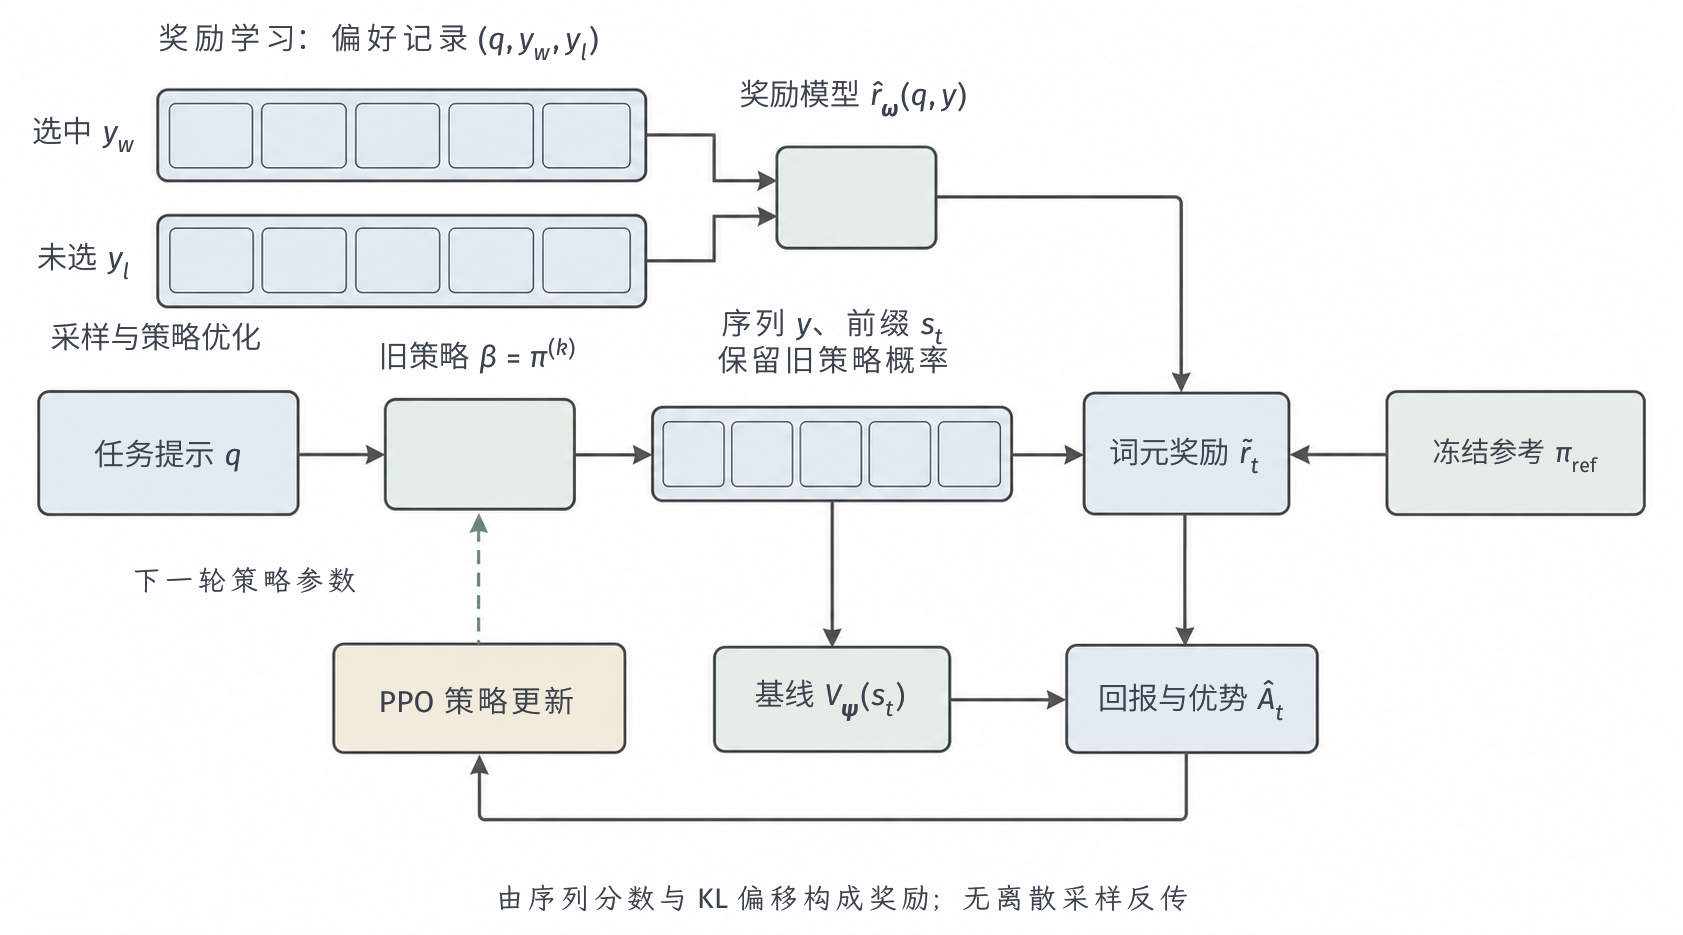
\includegraphics[width=157.400mm]{figures/10-reinforcement-learning/02-information-and-reward/generated/rl-reward-rlhf/figure.png}
  \caption{PPO式RLHF中的评价粒度。偏好标签训练完整回答评分器；旧策略逐token生成并记录采样概率，价值模型读取前缀提供基线。序列分数、旧策略概率与参考概率按式\eqref{eq:rl-reward-token-reward}构造逐token奖励，再经回报和优势估计进入策略更新；参考偏移不在更新器中重复计罚。图中连线表示回答、评分、采样概率及相应的训练信号，不表示通过离散采样端到端反向传播。图中省略部分批次字段连线：奖励模型评分仍读取本批$(q,y)$，PPO仍读取本批动作及旧策略概率。词元槽仅为示意，不规定回答长度。}
  \label{fig:rl-reward-rlhf}
\end{figure*}

逐token累加参考代价还会影响长短回答的权重。要把它与完整回答上的KL对应起来，可以使用序列概率分解所得的链式法则：
\[
  D_{\mathrm{KL}}(\pi(\cdot\mid q)\Vert\pi_{\mathrm{ref}}(\cdot\mid q))
  =\mathbb E_\pi\sum_{t<T}
    \log\frac{\pi(a_t\mid s_t)}{\pi_{\mathrm{ref}}(a_t\mid s_t)}.
\]
作为教学例，假设两个回答得分都为1，长度分别为2和4，各token的采样对数比恰好都是$0.1$。取$\lambda_{\mathrm{KL}}=0.5$，扣除参考代价后的样本分数分别为$0.9$和$0.8$。差异来自累加项，并不说明奖励模型明确偏好短回答；真实对数比也未必同号或恒定。若将KL或策略损失除以长度，就会改变长短回答的相对权重，而不是只做无影响的数值缩放。选择哪种聚合应依据任务标准，不能将一种归一化当成通用答案。

偏好标签不必都由人提供。Constitutional AI按照明确原则生成批评和修订，结合监督修订与AI偏好，再由AI偏好学习奖励、优化策略\scite{bai2022constitutional}
给定评分函数后，更换评价者不改变优化式的形式，却改变评分依据和误差来源，这些条件将在第~\ref{sec:rl-reward-sources}节检查。现在先固定奖励$r$，考察完整回答的概率分布如何在奖励与参考偏移之间取舍。下面在有限候选回答集合上优化全部概率分布，以便精确求解；实际网络只允许选择其参数可表示的分布，范围更小。

固定任务提示$q$，令$\mathcal Y$为有限非空的候选回答集合，$r(q,y)\in\mathbb R$，参考策略在每个候选上都满足$\pi_{\mathrm{ref}}(y\mid q)>0$，并取$\lambda_{\mathrm{KL}}>0$。在$\Delta(\mathcal Y)$上比较
\[
  F_q(\pi)=\mathbb E_{y\sim\pi(\cdot\mid q)}r(q,y)
   -\lambda_{\mathrm{KL}}D_{\mathrm{KL}}(\pi(\cdot\mid q)\Vert
                                    \pi_{\mathrm{ref}}(\cdot\mid q)).
\]
Gibbs变分结论表明，该目标的唯一最优分布是以参考概率为起点、按指数奖励重新加权：
\begin{equation}
  \begin{aligned}
    \pi^*(y\mid q)&=
      \frac{\pi_{\mathrm{ref}}(y\mid q)\exp(r(q,y)/\lambda_{\mathrm{KL}})}{Z(q)},\\
    Z(q)&=\sum_{z\in\mathcal Y}\pi_{\mathrm{ref}}(z\mid q)
                              \exp(r(q,z)/\lambda_{\mathrm{KL}}).
  \end{aligned}
  \label{eq:rl-reward-kl-optimum}
\end{equation}
有限集合、有限奖励与参考正支持保证$0<Z(q)<\infty$。这个结论把奖励差与最优策略相对参考策略的对数概率比联系起来，因而可用于随后将偏好拟合写成策略目标；它不保证参数化网络能够表示$\pi^*$。相关分布优化结论可参考\BookChapterRef{chap:information-theory-and-statistical-geometry}{卷2《数学准备：概率、因果与决策》的“概率分布的分析与优化”章}。

最优解并不把全部概率放在最高分回答上，而是以参考概率为起点，按$\exp(r/\lambda_{\mathrm{KL}})$重新加权。假设两个回答的参考概率都是$1/2$，奖励为$(\log3,0)$，$\lambda_{\mathrm{KL}}=1$，则$Z=2$，最优概率为$(3/4,1/4)$。若参考策略给某回答零概率，任何有限KL的策略也必须给它零概率，此时只能在参考支持内优化，不能沿用全回答空间的正支持结论。

从指数加权式取对数，得到$\log(\pi^*/\pi_{\mathrm{ref}})=r/\lambda_{\mathrm{KL}}-\log Z(q)$，于是奖励可写为“相对参考的对数概率”加$\lambda_{\mathrm{KL}}\log Z(q)$。后一个量对同一提示的所有回答相同。成对比较只需要奖励差，因此共同项恰好消去；这才使偏好拟合可以直接写成策略概率的目标，不是无条件地将奖励模型删掉。

这个精确解还提供了另一种偏好拟合方式。假定同一任务提示的偏好满足以$r$为效用的Bradley--Terry模型，便可把奖励差改写为最优策略相对参考策略的对数概率比差：
\begin{equation}
  \begin{aligned}
    r(q,y_{\mathrm w})-r(q,y_{\mathrm l})
    =\lambda_{\mathrm{KL}}\left[
      \log\frac{\pi^*(y_{\mathrm w}\mid q)}
                    {\pi_{\mathrm{ref}}(y_{\mathrm w}\mid q)}
      -\log\frac{\pi^*(y_{\mathrm l}\mid q)}
                    {\pi_{\mathrm{ref}}(y_{\mathrm l}\mid q)}
    \right].
  \end{aligned}
  \label{eq:rl-reward-dpo-change}
\end{equation}
其中$y_{\mathrm w}$和$y_{\mathrm l}$分别表示胜出和落选回答。同一任务提示的两边都有$\lambda_{\mathrm{KL}}\log Z(q)$，所以作差后消去；不同任务提示的归一化常数通常不能抵消。于是可以直接用策略概率比预测偏好，而不单独拟合奖励。以参数化策略替代$\pi^*$，将方括号内的量记为$z_{\bm{\theta}}(q,y_{\mathrm w},y_{\mathrm l})$，再最小化胜出标签的负对数似然，就得到\term{直接偏好优化}（direct preference optimization, DPO）：
\begin{equation}
  L_{\mathrm{DPO}}(\bm{\theta})
  =-\mathbb E_{(q,y_{\mathrm w},y_{\mathrm l})\sim\widehat P_{D_{\mathrm{pref}}}}
         \log\sigma\!\left(\lambda_{\mathrm{KL}} z_{\bm{\theta}}\right).
  \label{eq:rl-reward-dpo}
\end{equation}
期望在固定偏好记录$D_{\mathrm{pref}}$上计算，每条记录含同一任务提示及其胜出、落选回答。一次更新计算两条完整回答在当前策略和固定参考下的对数概率，再按式~\eqref{eq:rl-reward-dpo}下降；这个步骤既不采集新轨迹，也不训练显式价值模型。单条记录的梯度为
$-\lambda_{\mathrm{KL}}\sigma(-\lambda_{\mathrm{KL}} z_{\bm{\theta}})
[\nabla\log\pi_{\bm{\theta}}(y_{\mathrm w}\mid q)
-\nabla\log\pi_{\bm{\theta}}(y_{\mathrm l}\mid q)]$。
沿负梯度更新，局部方向提高胜出回答相对落选回答的对数概率。沿用均匀参考的双回答例，策略logit差就是$z$；当$z=0$且$\lambda_{\mathrm{KL}}=1$时，梯度为$-1/2$，以$0.2$为步长下降后$z=0.1$，胜出回答的概率约为$0.525$\scite{rafailov2023dpo}

DPO比较的是相对参考的变化，而非只看当前回答概率。另设两个回答的参考概率为$(0.8,0.2)$，当前概率为$(0.6,0.4)$，第一个是偏好标签中的胜者。两相对比为$0.75$和2，因此$z=\log(0.75)-\log2=\log(3/8)$。取$\lambda_{\mathrm{KL}}=1$，模型的胜出比较概率为$3/11\approx0.273$，即使当前第一个回答概率0.6仍高于第二个0.4。这个双回答例子说明偏好边际和动作概率是两个对象，更新关注相对参考提升了哪一个回答。

显式奖励模型加PPO，要给新采样回答评分并更新策略；标准DPO只在固定偏好比较记录上优化分类式损失。两者使用的训练记录和学习对象不同。上述换元解释了DPO与KL正则化最优策略的联系，却没有把DPO变成通常意义上的在线强化学习。实际模型类未必能表示$\pi^*$，有限记录未必覆盖所有回答，偏好也未必满足Bradley--Terry假设，所以不能由理想关系推出精确恢复最优策略。若在外层反复采样、标注再运行DPO，便形成迭代式偏好学习；在线访问和能区分候选奖励的新反馈来自外层协议，不来自分类损失本身。

% Outline: 5.2.5
\subsection{从过程与结果验证构造策略更新}
\label{sec:rl-reward-verification}

如果任务有明确的标准答案或可执行的产物，我们还可以绕开“逐对询问偏好”，直接检查候选是否满足某些条件：运行程序测试、按等价规则比对数学答案、或核对配送是否正确签收。这类检查可以反复使用同一标准，但它只能评价实际被检查到的那一个条件，不能因为几项检查通过就断言整个任务都已正确完成。

\begin{definition}[过程反馈与结果反馈]
  \label{def:rl-reward-verification}
  \term{结果反馈}（outcome feedback）评价行为结束后的产物或状态，例如答案是否等价、包裹是否正确签收。\term{过程反馈}（process feedback）评价中间状态、动作或步骤间关系，例如装载后身份是否一致、推导是否由前提合法推出。\term{可验证奖励}（verifiable reward）由明示验证规则产生；其可验证性依赖这条规则、检查时采用的前提和检查实现，不表示完整行为目标已经得到验证。
\end{definition}

过程与结果提供的证据也不能相互替代。推导可能使用非法除法却偶然得到正确答案，所以结果通过不足以证明过程有效；反过来，每步合法的变换也可能只是在反复改写题目，没有回答问题。表~\ref{tab:rl-reward-verifiers}据检查对象和前提比较验证器，自动检查是否可信仍要逐项判断。

\begin{table*}[htbp]
  \centering\small
  \begin{tabularx}{\linewidth}{@{}>{\raggedright\arraybackslash}p{21mm}*{4}{>{\raggedright\arraybackslash}X}@{}}
    \toprule
    检查器 & 可检查对象 & 检查前提 & 反馈粒度 & 主要漏检 \\
    \midrule
    规则验证器 & 格式、身份、答案等价 & 解析与等价规则符合标准 & 字段、步骤、结果 & 格式正确但内容错误；解析漏洞 \\
    执行器 & 代码、操作的实际结果 & 沙箱、程序测试用例、执行环境有效 & 工具调用或整次运行 & 未执行的程序测试用例、超时与资源副作用 \\
    形式检查器 & 形式命题及证明 & 形式化忠实，公理和检查内核可信 & 推理步骤、完整证明 & 证明了错误形式化的命题 \\
    模型评判器 & 开放式内容与解释 & 训练覆盖、提示及标准适用 & 片段、回答 & 风格偏好、位置偏差、共同模型盲点 \\
    \bottomrule
  \end{tabularx}
  \caption{四种验证器实际检查的对象及漏检范围。执行测试只支持所执行的程序测试用例，形式检查只支持所形式化的命题；两者都不能自行证明完整需求已被正确检查。}
  \label{tab:rl-reward-verifiers}
\end{table*}

拿到候选的验证得分后，可以比较同一任务提示下多个回答，为策略提供相对信号。\term{组相对策略优化}（group relative policy optimization, GRPO）以这组回答的得分为基准，给高于组均值的回答正信号，给低于均值的回答负信号，从而不必另拟合价值基线。沿用有限序列的未折扣评价，令旧策略$\beta$对$q$独立采样$m$个回答$y_i$，其验证或奖励模型得分记为$v_i$；这里$i$编号候选，不是$r_t$中的动作时刻。为中心化得分并统一组内尺度，定义
\begin{equation}
  \bar v=\frac1m\sum_{i=1}^m v_i,\qquad
  s_v=\sqrt{\frac1m\sum_{i=1}^m(v_i-\bar v)^2},\qquad
  \widehat A_i=\frac{v_i-\bar v}{s_v+\epsilon_{\mathrm{num}}},
  \label{eq:rl-reward-grpo-advantage}
\end{equation}
标准差使用分母$m$，$\epsilon_{\mathrm{num}}>0$防止分母为零。结果监督时，同一个$\widehat A_i$可以用于回答$i$的全部token，但它只表示该回答相对本组得分的高低，既不是逐token标签，也不是对状态价值函数的估计。

若两个回答都先完成相同的身份核对，随后一个正确装载、另一个拿错包裹，终局得分可以分别为1和0。组内信号会给第一条完整回答正值、第二条负值，连共同的核对步骤也使用不同符号。它适合推动完整行为概率，却不能据此判断核对在第二条轨迹中是错误动作；要作这种局部判断，仍需过程证据或有依据的归因。

为了将这个组信号接入策略更新，令$T_i$为回答长度，$\varrho_{i,t}=\pi_{\bm{\theta}}(y_{i,t}\mid q,y_{i,<t})/
\beta(y_{i,t}\mid q,y_{i,<t})$为当前与旧策略的token概率比，$\ell_{i,t}^{\mathrm{clip}}$为式~\eqref{eq:rl-reward-ppo}中以$\widehat A_i$替代$\widehat A_t$的剪裁项。一个常见实现先在每个回答内平均token项，再在组内平均，并扣除参考偏移代价，最大化代理目标
\begin{equation}
  \widehat{\mathcal L}_{\mathrm{GRPO}}
  =\frac1m\sum_{i=1}^m\frac1{T_i}
      \sum_{t=0}^{T_i-1}
       \left(\ell_{i,t}^{\mathrm{clip}}-\lambda_{\mathrm{KL}} k_{i,t}\right),
  \label{eq:rl-reward-grpo}
\end{equation}
其中$k_{i,t}$是所选参考KL估计或局部近似，常用形式为
$k=\exp(-\ell)+\ell-1$，$\ell=\log(\pi_{\bm{\theta}}/\pi_{\mathrm{ref}})$；
若当前策略和参考策略在同一合法token集合上都为正，且动作由$\pi_{\bm{\theta}}$采样，那么给定前缀有$\mathbb E_{\pi_{\bm{\theta}}}\exp(-\ell)=1$，从而$k$的期望等于前向KL。旧策略采样不自动满足这个分布条件；复用旧样本时若没有分布校正，样本平均就不能当成精确KL，更不能证明硬约束成立。长度平均、剪裁和采样KL都属于代理目标的选择，与无近似的期望奖励梯度需要区分。

GRPO中选用的$k$还区分了样本值与期望值。普通对数比$\ell$可以为负；而$e^{-\ell}\geq1-\ell$给出$e^{-\ell}+\ell-1\geq0$，所以这种样本项每次都非负。它的KL含义仍依赖正确的动作抽样分布，非负并不使旧策略样本平均自动成为当前策略的精确KL。计算形式与概率依据需要分别检查。

\begin{example}[一组验证得分的更新信号]
  \label{ex:rl-reward-grpo}
  假设$m=4$，四个得分为$(1,1,0,0)$，则$\bar v=0.5$、$s_v=0.5$。忽略极小稳定项，相对信号为$(1,1,-1,-1)$。为计算一次更新，再设任务只有一步和两个动作，成功动作概率为$p=\sigma(z)$，当前$z=0$，不加KL惩罚，概率比处在未剪裁区。这组样本对logit的梯度为
  \[
    \frac14\{2(1)(1-p)+2(-1)(-p)\}=\frac12.
  \]
  用$0.2$为步长上升，得到$z'=0.1$，成功动作概率约为$0.525$。若整组全为1或全为0，中心化后的分子都为0；稳定项只能使计算有限，不能产生奖励梯度。若实现保留KL项，正则化仍可能产生梯度。
\end{example}

标准化还改变不同结果的相对幅度。若四个分数为$(1,0,0,0)$，均值为$1/4$，标准差为$\sqrt3/4$；忽略数值稳定项，成功样本信号为$\sqrt3$，三个失败样本各为$-1/\sqrt3$。这与前面两个成功、两个失败时的$\pm1$不同。更大幅度来自本组成功比例较低，并不表示检查器证明这次成功更重要或各步骤贡献更大。

上述算例给出的是组内相对信号，不能直接当作无偏真实优势。即使不除以标准差，组均值含样本自身也会改变梯度期望。为了看清这一点，固定$q$和得分函数$v$，从$\pi$独立同分布采样，记$\bm g_i=\nabla\log\pi(y_i\mid q)$。利用$\mathbb E\bm g_i=0$，可得
\[
  \mathbb E\left[\frac1m\sum_i(v_i-\bar v)\bm g_i\right]
  =\left(1-\frac1m\right)\nabla\mathbb E_\pi v.
\]
缩放因子来自$\bar v$中与$\bm g_i$相关的自身得分，其余独立样本的交叉期望为零。再除以随机$s_v$，还会引入与组内成功比例有关的权重；二值奖励混合组中，较少见结果的标准化绝对值更大。改用不含自身的组均值可以消除这个特定缩放，但不能同时消除标准化、剪裁或复用旧样本造成的偏差。

“组均值作基线”与前章动作前固定基线的条件不同：这份均值包含正在被加权样本的自身得分，因而与其概率梯度相关。独立的其他回答部分会在期望中抵消，自身那一份却扣掉了$1/m$的梯度；所以即使只中心化也会出现上面的缩放。数值稳定或每项非负并不修复这种统计依赖，重复使用旧策略样本还要另查分布校正。

组内比较只要求给出$v_i$，并未规定它必须来自规则。DeepSeekMath提出GRPO，并讨论结果奖励模型、过程奖励模型和迭代刷新，反馈并不限于规则判分\scite{rl5-shao2024deepseekmath}
DeepSeek-R1原始技术报告中的R1-Zero及R1推理训练使用正确性、格式等规则奖励；但R1完整多阶段流程还包含监督微调及用于通用任务回答的模型奖励，不能用推理阶段的反馈概括全部训练\scite{deepseek2025r1}

\term{基于可验证奖励的强化学习}（reinforcement learning with verifiable rewards, RLVR）说明奖励由明示规则产生，GRPO则说明拿到分数后如何更新策略，两者不是同一个分类依据。验证器将未满足条件的候选判为通过，称为假阳性（false positive）；解析偏差、测试泄漏或长度与表达偏好也可能被策略用来增加得分。增加同一任务提示的采样数可提供更多组内比较，却不会补齐未检查要求。在多轮工具任务中，还要明确评分针对动作格式、工具执行还是最终完成情况；将终局成功平均分给工具调用，并没有取得独立的动作正确性标签。更长交互的前沿问题见第~\ref{chap:rl-overview}章，语言模型实现由应用卷承接。

% Outline: 5.2.6
\subsection{反馈来源与目标可识别性}
\label{sec:rl-reward-sources}

回到配送任务，已有示范可能足以复现动作，偏好记录可能足以预测路线胜负，验证器可能足以判断签收身份。要判断目标是否可识别，必须先指定想要哪种结论，再检查产生同样反馈的候选解释是否都支持它。奖励即使不唯一，候选奖励也可能一致支持当前动作；偏好即使预测准确，也不能说明未被评价的要求已经学会。这正是前章可识别性在目标反馈上的应用。

同一对行为的胜负标签可以由人判断，也可以由模型判断。比较这两种来源，主要要检查判断依据、成本和误差是否相同，而不是仅比较记录格式。形式相同不意味着评价质量相同。

\term{基于AI反馈的强化学习}（reinforcement learning from AI feedback, RLAIF）由AI承担部分评价，再用所得反馈学习策略。\term{原则指导反馈}（constitutional feedback）则以明确原则指导评价或修订，用这些原则产生批评、修订示范或偏好。前者说明评价来源，后者说明判断依据；原则不是与示范、偏好互斥的记录类型，其选择仍须由外部目标约定。

\begin{table*}[t]
  \centering\small
  \begin{tabularx}{\linewidth}{@{}>{\raggedright\arraybackslash}p{22mm}*{5}{>{\raggedright\arraybackslash}X}@{}}
    \toprule
    来源或协议 & 判断依据 & 相关偏差 & 可追溯性 & 查询成本 & 外部校验 \\
    \midrule
    人类反馈 & 任务知识、个人偏好、指南 & 疲劳、群体差异、顺序效应 & 需保留指南与标注群体 & 人工时间 & 交叉复核、真实结果 \\
    RLAIF & AI知识与提示中的标准 & 共享训练偏差、风格偏好 & 需记录模型和提示版本 & 推理及抽查成本 & 独立人评、规则或执行 \\
    原则指导反馈 & 显式原则及其解释 & 原则遗漏、冲突解释 & 原则可见不等于执行透明 & 原则维护与评价成本 & 逐原则反例测试 \\
    模型评判器 & 学得评分或比较函数 & 分布外失准、位置与长度偏差 & 需记录反馈模型的训练样本组成及模型版本 & 批量打分与刷新 & 留出来源、实物或程序检查 \\
    \bottomrule
  \end{tabularx}
  \caption{反馈来源及协议的判断依据、成本与校验方式。RLAIF可使用原则指导的模型评判器，因此同一系统可以同时属于多行，不能按互斥类别解读。}
  \label{tab:rl-reward-sources}
\end{table*}

假设人工标注员和模型都只看终点照片，两者都判断“已送达”，却都看不到包裹内部破损。增加来源一致性没有增加包裹内部破损的检查记录，因此不能推出包裹完好。来源分歧也未必是噪声：一位收件人看重速度，另一位看重省电，可能确实采用不同取舍，不应直接删除其中一方的反馈。

表~\ref{tab:rl-reward-sources}列出的外部校验，也应注明被评价行为的任务条件和适用范围。评价器只在身份、路线条件等必要字段齐全的短距离配送记录上检查过，就不能直接用于长路线、身份缺失或新包裹，并声称同样可靠。现有证据只支持已检验策略在这些配送条件和评价标准下的结论；要判断多个奖励解释是否会造成实际失配，还要比较未见行为上的排序。

% Outline: 5.3
\section{奖励归因受限下的强化学习}
\label{sec:rl-reward-credit}

假设我们已经约定了“配送成功”的确切含义、也能拿到可靠的终局反馈，剩下的问题是：怎样用这一个结果去更新核对、装载等早期动作。此时目标与反馈语义都已固定，但结果回溯、过程判断、奖励变换和辅助目标这几种做法改变的学习对象并不相同：有的需要新增步骤标签或专家评价，有的只是改变记账方式或训练安排；它们能否保持原目标，所要求的条件也各不相同。

% Outline: 5.3.1
\subsection{基于长期结果回溯构造局部学习信号}
\label{sec:rl-reward-redistribution}

在四步配送中，早期核对决定是否拿对包裹，中间搬运可能只是执行既定方案。REINFORCE或多步回报能将终局成功用于核对动作的更新，但搬运和提示播放也可能收到同一个成功回报。前章的基线和自举分别减少共同波动、缩短传播路径，并没有直接测量“改变这个动作会使结果变化多少”。这里回用第~\ref{chap:rl-learning}章的估计方法，进一步检查局部信号所表达的贡献。

\term{奖励重分配}（reward redistribution）将同一结果重新记到轨迹上的不同位置，使结果与关键事件的时间联系更短。要判断这种记账是否仍优化原目标，必须按原来的折扣权重比较整条轨迹的新旧奖励，而不能只比较未折扣总和。若要求逐轨迹保持回报，应满足
\begin{equation}
  \sum_{t=0}^{H-1}\gamma^t\widetilde r_t
    =\sum_{t=0}^{H-1}\gamma^t r_t.
  \label{eq:rl-reward-redistribution}
\end{equation}
逐轨迹相等足以保持每个策略的期望回报；也可以使用较弱条件，但需要期望相等对全部待比较策略成立。另要检查信号何时可得。依赖整段历史的新奖励通常不是原状态上的马尔可夫奖励，需要相应表示；若它依赖记账时刻之后才发生的结果，只加入过去历史仍不能使反馈当时可得。

例如$H=4$、$\gamma=0.9$，原奖励$(0,0,0,1)$对应初始回报$0.9^3=0.729$。若全部移至$t=0$，新奖励应为$(0.729,0,0,0)$；若移至$t=1$，则应为$(0,0.81,0,0)$，两者按折扣计算仍为$0.729$。直接移成$(1,0,0,0)$只保留未折扣总和，没有保留原目标。若轨迹长度可变，同样忽略折扣还会改变快慢路径的排序。

保持总回报也不意味着可以直接用新奖励计算reward-to-go，即从当前动作起的后续奖励回报，包含该动作的奖励。假设终局成败取决于最后一个动作，却将全部结果事后记到$t=0$，末步的局部回报就变为0，用它更新末步策略会丢掉该动作的影响。第~\ref{chap:rl-learning}章之所以能删去过去奖励，是因为过去结果不受当前动作影响；事后前移的信号不满足这个因果条件。将不变的完整轨迹回报与整条轨迹的对数概率梯度相乘，仍保留原目标梯度。要改用局部更新，还须另外证明重分配与估计器的配套条件。

这个失效可用四步任务的最后一次交付手算。前面三步固定，末步选择正确收件人的概率为$p=\sigma(\theta)$，成功得1、失败得0，$\gamma=0.9$。原起点目标是$J=0.729p$，导数为$0.729p(1-p)$。若事后把成功分全部记成$t=0$的$0.729$，总目标仍相同，但末步之后的重分配回报为0；用它乘末步对数概率梯度会给出零更新。完整轨迹回报仍含末步结果，乘它的对数概率梯度才能保留原导数。过去奖励可被删去所需的因果条件，不能只由总和相等推出。

一种重分配依据是观测、动作前缀对最终回报预测的影响。令$m_t$预测看到前缀后的最终回报，将$m_t-m_{t-1}$视为读入新一步记录后的回报预测增量；取$m_{-1}=0$且$m_{H-1}=G_0$，相邻差求和恰为$G_0$。若将其记为折扣局部奖励，且$0<\gamma\leq1$，可取$\widetilde r_t=\gamma^{-t}(m_t-m_{t-1})$以抵消记账位置的折扣。末端预测不等于真实回报时必须补残差，否则总回报也改变了。实际学习还需控制预测误差和$\gamma^{-t}$的放大；RUDDER用回报预测与贡献分析构造信号，其机制入口已在第~\ref{chap:rl-learning}章介绍。

回报预测增量仍不等于改变动作所产生的干预贡献。假设正确核对后屏幕总会闪光，日志中闪光与成功高度相关；但关闭闪光不会改变交付，拿错包裹才会导致失败。归因模型只依据相关性时，可能把奖励分给闪光。检验应改变无关标记、受控比较关键动作，并观察实际交付结果；仅有回报预测误差下降不足以证明贡献判断正确。对动作干预作比较，还要固定动作前的共同条件，说明允许的干预及其后续执行规则，并检验支持与相应的混杂控制条件；单纯的预测增量没有提供这些条件。这个区分用于判断局部奖励信号能否解释动作贡献，可参考\BookChapterRef{chap:causal-inference}{卷2《数学准备：概率、因果与决策》中讨论因果响应的章节}。

% Outline: 5.3.2
\subsection{基于过程反馈构造局部学习信号}
\label{sec:rl-reward-process}

若终局日志无法区分核对错误与中途换包，可以新增装载前的身份检查。这个检查提供新的中间证据，而不是将原总分分摊到各步。需要先明确它评价什么：读码动作、装载后的身份关系和到达时的包裹状态对应不同决策，只有步骤边界和被检关系清楚，才能确定反馈监督的对象。

图~\ref{fig:rl-reward-process}把人工标注、规则检查、执行记录和模型步骤评价放到同一轨迹中，标明各自覆盖的步骤。例如执行记录只证明包裹放入箱内，不证明身份正确；模型觉得搬运平稳，也不能替代破损检查。推理任务中的逐步骤评价同样需要明确标签标准及标注范围。

在Lightman等的工作中，标注者按统一规范把数学解答的步骤判为正、负或中性。带标签的解答前缀成为训练样本，\term{过程奖励模型}（process reward model, PRM）学习在题目和已生成前缀给定时预测这三类标签的概率。训练对象是这个评价模型：只对已有步骤标签拟合分类概率，未被评价的步骤不能自动补成正例。模型预测的步骤分数还须聚合，才能比较两份完整解答\scite{lightman2023verify}。

过程奖励模型预测的是评价者会怎样判断当前步骤；价值模型预测的是该前缀之后的累计回报。一步被判合法，不表示后来一定解对题目，也不直接给出这步相对其他动作的优势。要将这些分类概率用于整解排序或训练，需要另选聚合规则，并说明它对应什么问题。

设题目为$q$，一份候选解为$c=(c_1,\ldots,c_m)$，$m$是其步骤数。按该论文的主要评分约定，将中性与正类合并；令$p_j$为模型根据$(q,c_{1:j})$预测第$j$步属于这两类的概率，整解排序分数为
\begin{equation}
  F_{\mathrm{PRM}}(q,c)=\prod_{j=1}^{m}p_j.
  \label{eq:rl-reward-prm-score}
\end{equation}
例如两份两步解的预测概率分别为$(0.9,0.9)$和$(0.99,0.6)$，分数为$0.81$与$0.594$，会选择前者。这个乘积是评价模型的排序规则，不能仅凭相乘就解释为全部步骤正确的真实联合概率；步骤较多时，乘积也可能因长度而降低。原文还比较了取最小步骤分数及不同中性处理的选择，它们改变的是整解排序方式，不是环境奖励的测量规则。

即使每步概率都准确，乘积也未必是全部正确的概率。设两步同时依赖一个共同前提，前提以$0.9$概率有效；有效时两步都正确，无效时两步都错误。两步各自正确概率都是$0.9$，共同正确概率却是$0.9$而非$0.81$。概率链式法则需要逐步条件于此前步骤都正确；一般PRM的步骤预测没有自动提供这种条件量。因此乘积可作排序规则，不能仅因每项像概率就认作真实联合成功率。

在候选筛选评价中，生成器保持固定，对每道测试题采样$n$份完整解，再交付$F_{\mathrm{PRM}}$最高的一份，这就是best-of-$n$选择。它既要支付$n$次生成成本，也要评价这些候选的步骤；报告选择效果时必须固定生成器、采样预算和测试范围。该论文的主要比较按最终答案检查被选解的成功率，支持的是这一筛选用途，不能直接写成策略梯度训练带来的收益。若随后用步骤分数更新生成策略，还须另行规定采样策略、局部归因和优化目标；步骤判断概率本身不是状态价值或真实优势，过程奖励模型也没有普遍优于结果奖励模型的保证。

即使各处检查都通过，局部正确也可能没有组成全局成功。机器人每次搬运都遵守速度限制、每次放置都平稳，却只在两个中间站往返，没有交给收件人。过程条件没有覆盖最终交付；若各次身份检查只看单个字段，还可能遗漏跨步骤身份一致性。因此，将局部分数求和之前要解释它与整体要求的关系，终局检查不能仅因步骤有标准就取消。

过程反馈也增加获取和维护成本：标注量通常随步骤数增长，不同标注者还可能采用不同的步骤切分。模型反馈若有系统偏差，会在多个位置重复传入更新。可以比较只补关键步骤与标注全部步骤所需成本，统一标准版本，再检查独立交付结果是否改善。若发现检查标准遗漏了要求，就需要修订目标标准，不能只调整局部信号权重。

\begin{figure*}[htbp]
  \centering
  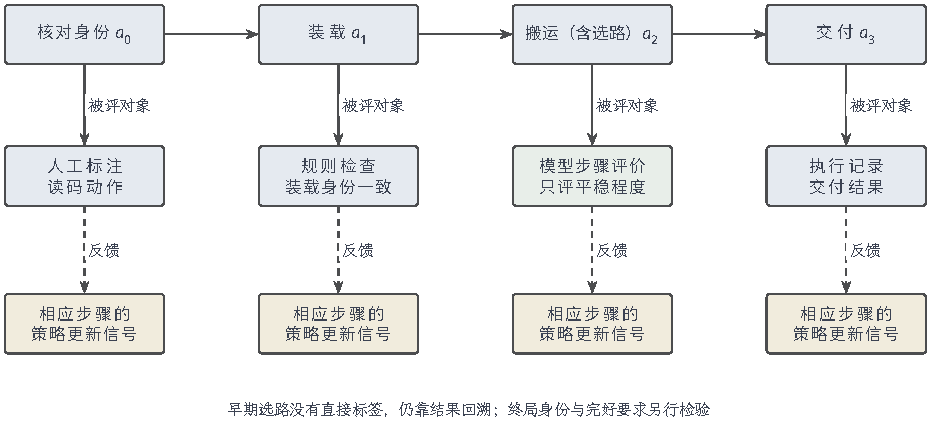
\includegraphics[width=157.618mm]{figures/10-reinforcement-learning/02-information-and-reward/tikz/rl-reward-process.pdf}
  \caption{过程反馈缩短部分决策到评价的路径。上方为按时间执行的配送步骤，下方为评价来源；由反馈指向更新对象的虚线表示学习信号。未标注步骤仍依赖终局回报传播，局部通过不取代最终身份和完好检查。}
  \label{fig:rl-reward-process}
\end{figure*}

% Outline: 5.3.3
\subsection{基于奖励变换构造局部学习信号}
\label{sec:rl-reward-shaping}

即使不增加任何新检查，也可以依据已有目标人为构造更即时的引导信号。例如希望鼓励机器人靠近终点，但简单地“只要靠近就加分”会被钻空子——机器人可以反复离开再靠近、不断领分。要避免附加分数任意改变长期目标，可以采用\term{潜势型奖励塑形}（potential-based reward shaping）：先给每个状态打一个“潜力分”，再只按与任务相同折扣的相邻潜力之差发附加奖励，使一段路途上的附加项能够逐项抵消。

\begin{definition}[潜势型塑形]
  \label{def:rl-reward-shaping}
  给定与任务相同的折扣$\gamma$及状态势函数$\Phi:S\to\mathbb R$，定义
  \[
    F(s,a,s')=\gamma\Phi(s')-\Phi(s),\qquad
    r'_t=r_t+\gamma\Phi(s_{t+1})-\Phi(s_t).
  \]
  $\Phi$是人为指定或从交互训练记录学习的状态评分，称为势函数；附加奖励必须采用这个折扣差形式，不能用任意启发式分数替代。
\end{definition}

折扣差为什么能避免给往返反复加分，可以先看两步。令起点势为0、近处势为1，$\gamma=0.9$；从起点到近处的附加奖励为$0.9$，再回起点为$-1$，折扣后的附加总和为$0.9+0.9(-1)=0$。只奖励靠近而不扣离开，会使同样往返拿到额外分。势差把同一中间状态在相邻两步中的贡献抵消，下面的推导把这个计算推广到整个轨迹并保留末端项。

为判断附加信号是否仍评价原任务，我们比较塑形前后的完整折扣回报。下面利用相邻势项相消，证明在给定条件下两者只差一个不依赖策略的期望常数；这是策略不变奖励变换的经典结论\scite{rl5-ng1999shaping}

\begin{theorem}[无限折扣时域的塑形不变性]
  \label{thm:rl-reward-shaping}
  设$0\leq\gamma<1$，固定所有待比较策略共同使用的有界可测状态势函数$\Phi:S\to\mathbb R$及初始分布$\mu_0$。假设各策略的原折扣回报作为随机级数几乎处处收敛，且所得实随机变量可积。则塑形后的回报几乎处处满足
  \[
    G'_0=G_0-\Phi(s_0),\qquad
    J'(\pi)=J(\pi)-\mathbb E_{\mu_0}\Phi(s_0).
  \]
  因而所有策略在标准期望折扣回报下的排序不变。
\end{theorem}

\begin{proof}
  先取长度为$H$的有限前缀，以便保留末端边界项。将塑形奖励代入折扣和，相邻势项逐项相消：
  \begin{align*}
    \sum_{t=0}^{H-1}\gamma^t r'_t
    &=\sum_{t=0}^{H-1}\gamma^t r_t
       +\sum_{t=0}^{H-1}
          \bigl[\gamma^{t+1}\Phi(s_{t+1})
                          -\gamma^t\Phi(s_t)\bigr]\\
    &=\sum_{t=0}^{H-1}\gamma^t r_t
       -\Phi(s_0)+\gamma^H\Phi(s_H).
  \end{align*}
  由$|\Phi(s)|\leq M$，末端项绝对值至多为$\gamma^H M$，当$H$趋于无穷时消失；若$\gamma=0$，从$H\geq1$起该项就为零。因此在原折扣级数收敛的轨迹上满足$G'_0=G_0-\Phi(s_0)$。势的有界性保证差值可积，取期望得到只依赖共同初始分布的偏移。任意两策略减去同一个期望数值，其回报差和排序均不变。
\end{proof}

保持期望排序不要求$\Phi$等于精确价值。即使势函数误将慢路线评为接近终点，只要有界且按同一折扣差加入，定理仍成立；但错误势值可能妨碍学习，使速度或有限样本回报变差。若初始状态随机，$-\Phi(s_0)$也是随机偏移，可能改变方差及\term{条件风险价值}（conditional value-at-risk, CVaR）这类尾部评价。以损失$-G_0$定义CVaR时，它评价上尾的大损失，对应回报较差的结果。第~\ref{chap:rl-trustworthy}章的风险目标需要另查不变性，不能继承这里的期望结论。

有限任务没有无穷尾项可供消去，必须保留终端势。允许势随时刻变化，采用
$r'_t=r_t+\gamma\Phi_{t+1}(s_{t+1})-\Phi_t(s_t)$。
沿相同方式展开，可得
\begin{equation}
  \sum_{t=0}^{H-1}\gamma^t r'_t
  =\sum_{t=0}^{H-1}\gamma^t r_t
      -\Phi_0(s_0)+\gamma^H\Phi_H(s_H).
  \label{eq:rl-reward-shaping-terminal}
\end{equation}
这个恒等式也适用于有限时域的$\gamma=1$。令$\Phi_H=0$足以消去末端项；若$H$固定，终端势为所有策略共享的常数也能保持排序。$\gamma=0$时末端项不影响目标，但其他折扣下必须显式处理边界。

自然终止和采样时间截断对应不同边界。自然终止后不再记账时，应将终止势设为零，或显式抵消$\gamma^T\Phi_T(s_T)$；若$T$可变且$\gamma<1$，即便终端势都是同一非零常数，折扣后的末端项也会随长度变化。若采用吸收状态并无限继续记塑形奖励，尾项可以继续相消，但不能只记进入吸收状态的一步，省略随后塑形项。训练批次截断则可能尚未结束任务，需要保留原续接价值和对应塑形价值$V'(s)=V(s)-\Phi(s)$；若不保留，就要明示改求有限时域目标。未计算续接价值不意味着它为零。

\begin{example}[遗漏终端势会改变排序]
  \label{ex:rl-reward-terminal}
  假设$H=1$、$\gamma=0.9$，从同一起点选择到终点甲或乙，原奖励都是0，且$\Phi_0(s_0)=0$。若$\Phi_1(\text{甲})=1$、$\Phi_1(\text{乙})=0$，到达后立即停止记账，新回报分别为$0.9$和0，原本并列的路径变成甲更优。将两个终端势都设为0则消除了这一差异；在含中间步骤的任务中，即使中间势不准确，只要满足相应定理条件，仍可保持期望排序。
\end{example}

现在可以具体区分这些保持条件。潜势塑形使共同起点的回报只差固定势值，重分配可以要求逐轨迹折扣回报完全相同，一般辅助奖励则不自动具有这两种性质。即使附加信号更密集、代数上保持了目标，也没有证明它等于动作的因果贡献。

% Outline: 5.3.4
\subsection{基于辅助目标构造局部学习信号}
\label{sec:rl-reward-auxiliary}

“给学习增加辅助信号”有两种作用位置完全不同的做法，必须分清。让机器人预测下一时刻的位置，是用预测误差训练状态表示，促使它保留用于后继预测的特征，行为最终仍按原任务回报评价；而为“每次到达装载区”加分，则是直接改变了策略优化的回报。两者都可能改变学习速度，但前者作用于表示、后者作用于计分，并非等价。是否更快达到同一原任务回报，或是否改善原任务，还需在相同采样与计算预算下分别检验。

为说明更新位置，设共享表示参数为$\bm{\eta}$，任务的策略或价值损失为$L_{\mathrm{task}}$，下一状态预测损失为$L_{\mathrm{aux}}$。以$\lambda$设置辅助损失权重、$\alpha$为步长，联合更新为
$\bm{\eta}^{(k+1)}=\bm{\eta}^{(k)}
-\alpha\nabla_{\bm{\eta}}(L_{\mathrm{task}}+\lambda L_{\mathrm{aux}})$。
辅助预测梯度改变共享表示，最终行为仍按原任务回报评价。若改为给动作增加辅助奖励$b_t$，采用$r'_t=r_t+\lambda b_t$，则优化目标变为
$J'(\pi)=J(\pi)+\lambda\mathbb E_\pi\sum_t\gamma^t b_t$，
除非$b_t$满足额外不变条件，这个新目标不再等于原任务。图~\ref{fig:rl-reward-auxiliary}将两条路径分别接到共享表示和回报，显示它们改变的对象。

\begin{figure*}[htbp]
  \centering
  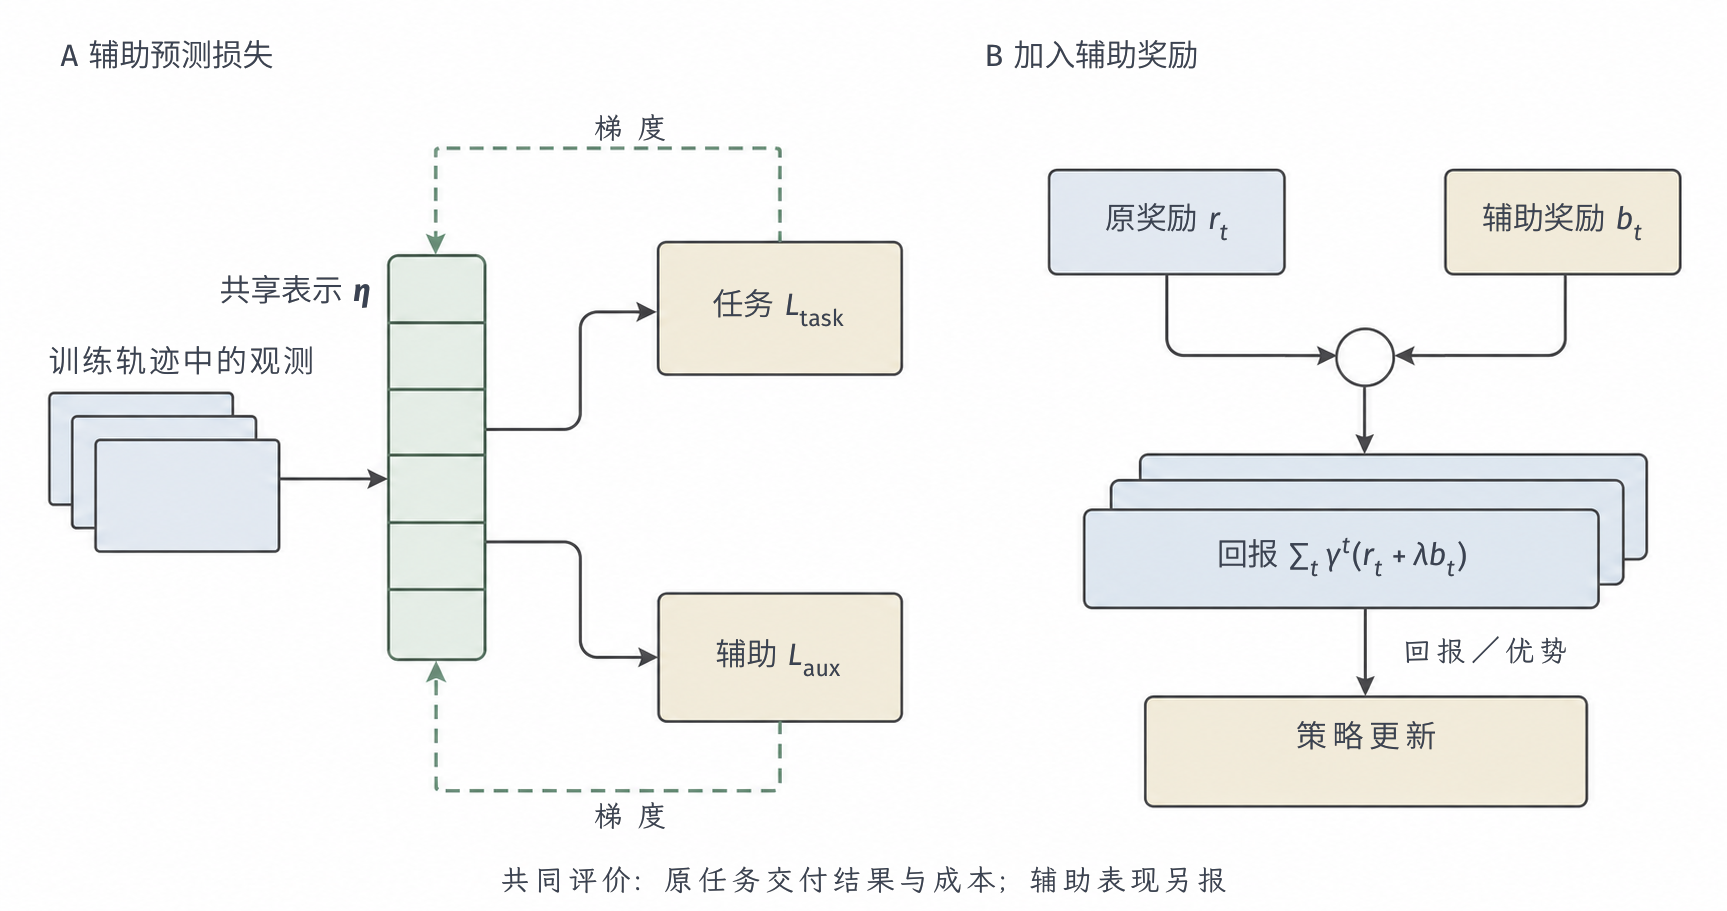
\includegraphics[width=157.400mm]{figures/10-reinforcement-learning/02-information-and-reward/generated/rl-reward-auxiliary/figure.png}
  \caption{辅助预测损失与辅助奖励的干预位置。左侧虚线为损失对共享表示的梯度；右侧辅助奖励先进入回报，再产生策略更新信号。两种训练的最终行为都应按未掺入辅助分数的原任务标准评价。帧、特征格与回报条带数量仅为示意。}
  \label{fig:rl-reward-auxiliary}
\end{figure*}

辅助梯度也可能与任务梯度冲突。用一个标量参数作教学例，令$L_{\mathrm{task}}=(\eta-1)^2/2$、$L_{\mathrm{aux}}=(\eta+1)^2/2$。在$\eta=0$，两梯度为$-1$与1；若辅助权重为1，合成梯度为0，尽管任务损失尚未最小。这个例子不说明所有辅助预测都会妨碍学习，而是说明共享参数和增加监督，并没有自动保证任务优化方向得到改善。

另外两种训练安排也需区分。训练课程改变任务分布，例如先练短路线，再增加距离；人为子目标改变决策组织，例如先到装载区，再去收件处。二者都不必增加奖励，也不等于潜势塑形。时间抽象回用第~\ref{chap:rl-learning}章；目标重标记及\term{事后经验回放}（hindsight experience replay, HER），即将轨迹按实际达到的目标重新使用，由第~\ref{chap:rl-transfer}章展开。

若进入装载区就给辅助分，机器人可能反复进出而不交付，因为计分没有限制重复次数，也未要求主任务进展。调整$\lambda$、切换课程或移除辅助信号后，应分别检查原始交付成功、辅助预测误差和子目标完成情况，不能用辅助分的上涨替代主任务收益。表示预测更准确也不证明动作贡献判断正确；共享参数上的辅助梯度还可能与任务梯度冲突。

% Outline: 5.3.5
\subsection{奖励归因方法的误差与适用边界}
\label{sec:rl-reward-credit-boundaries}

同一终局结果可以回溯记账，可以补充过程检查，也可以与塑形或辅助目标结合。要在这些办法间选择，我们需要比较步骤标签、专家评价或转移记录的获取成本、局部信号的含义和原目标的保持条件。表~\ref{tab:rl-reward-credit-methods}按这几个共同对象对照四条路线。

\begin{table*}[htbp]
  \centering\small
  \begin{tabularx}{\linewidth}{@{}>{\raggedright\arraybackslash}p{23mm}*{5}{>{\raggedright\arraybackslash}X}@{}}
    \toprule
    路线 & 额外反馈成本 & 所需轨迹字段或预测量 & 局部信号 & 原目标保持条件 & 主要失效 \\
    \midrule
    长期结果回溯 & 可无新标签；需拟合 & 前缀、终局结果 & 回报预测变化或重分配 & 同一折扣下的回报相等，或全策略期望相等 & 相关标记代替贡献、残差遗漏 \\
    过程反馈 & 关键步骤标注或检查 & 被评步骤及上下文 & 局部评分或通过标记 & 若加入回报，须另证聚合后仍保持原策略排序 & 局部正确不能组合为成功 \\
    奖励变换 & 势函数构造成本 & 相邻状态、终止类型 & 折扣势差 & 有界势、共同初始分布、正确终端项 & 截断当终止、折扣不一致 \\
    辅助目标 & 预测标签、额外任务 & 观测编码或子任务标签 & 辅助梯度、额外奖励 & 预测损失不改评价；额外奖励另证等价 & 梯度冲突、子目标循环 \\
    \bottomrule
  \end{tabularx}
  \caption{奖励归因路线的适用条件。过程反馈和一般辅助奖励没有自动保持原目标的代数保证。}
  \label{tab:rl-reward-credit-methods}
\end{table*}

即使采用同一条路线，误差也可能来自不同环节。归因模型错误把已经明确的成功结果分给无关动作；有限样本误差使现有证据不足以区分贡献；反馈标准错误则使“成功”本身遗漏破损要求。增加样本可能减轻第二种误差，但不自动修正第一种模型假设，也不会让错误标准变完整。

可以在同一配送任务中固定策略架构与预算，分别检查这些缺口。移除身份过程标签后看身份错误是否重新出现，用来判断身份过程标签的作用；打乱不影响环境的屏幕闪光，再看局部信号和策略是否改变，用来检测相关性捷径。保持原奖励不变，核查自然终止和时间截断的势值处理，则可排除记账意外改变目标。各项检查都要记录原始交付结果及错误类型，不能只比较掺入辅助分的奖励曲线。通用信用传播仍由前章工具承担，本节补充其信号来源和语义；标准本身的缺口需要转向目标诊断。

% Outline: 5.4
\section{奖励与行为目标不匹配}
\label{sec:rl-reward-mismatch}

即使策略已经能拿到大量反馈、也能把终局分数传给早期动作，它仍可能在“分数很高”的同时完成了一次错误的配送。这时问题不在学习算法，而在计分标准与真正的行为要求之间出现了偏差。诊断这种偏差，需要先把行为要求和证据讲清楚，再实际检验具体行为、辨认偏差的根因，然后才有依据修订目标或估计方法；修订后还要用新产生的行为重新检测——只给奖励换个名字并不能解决偏差。

% Outline: 5.4.1
\subsection{明确行为目标和代理奖励}
\label{sec:rl-reward-proxy}

配送要求包括交给正确收件人、保持包裹完好，以及满足约定的代价条件，训练代理却可能只给终点图像打分。继续用同一个评分器评价策略，就仍看不到内部破损。表~\ref{tab:rl-reward-requirements}将每项要求与训练编码、独立证据和未覆盖条件对应；这种逐项检查能显示平均总分可能隐藏的遗漏。

\begin{table*}[htbp]
  \centering\small
  \begin{tabularx}{\linewidth}{@{}*{4}{>{\raggedright\arraybackslash}X}@{}}
    \toprule
    行为要求 & 训练编码 & 独立评价 & 未覆盖条件 \\
    \midrule
    交给正确收件人 & 终点照片评分 & 签收身份与包裹编号双重核对 & 照片不含身份时仍缺证据 \\
    包裹完好 & 平稳搬运过程分 & 独立开箱检查或有效传感记录 & 隐性破损与传感盲区 \\
    能耗可接受 & 电量成本或偏好权重 & 校准电表、同负载路线比较 & 新载荷、不同电池状态 \\
    按时交付 & 终局成功或到达时间分 & 固定截止时间下的完成记录 & 长尾延迟与未完成轨迹 \\
    \bottomrule
  \end{tabularx}
  \caption{先建立行为要求到证据的对应，再选择数值聚合。某项无法观测意味着结论受限，不意味着它可以从目标中消失。}
  \label{tab:rl-reward-requirements}
\end{table*}

完整记录要求也不意味着所有要求都能同时改善。例如高收益配送可能更耗电，单一总分已经替决策者选定了取舍。向量奖励保留各项目标的数值，再另行指定怎样比较它们，使权衡不被藏在总分中。

图~\ref{fig:rl-reward-pareto}采用四个教学候选：甲$(2,4)$、乙$(4,7)$、丙$(6,8)$、丁$(5,5)$，横、纵坐标分别为能耗和收益，所以向左上改善。乙比丁收益高且能耗低，两个指标都不吃亏，这称为乙支配丁；甲、乙、丙在这四个候选中没有被支配。若按“收益减能耗”比较，三者得分为2、3、2，就选择乙。

在共同的任务、初始分布与时域口径下，令$\bm r_t=(r_{t,1},\ldots,r_{t,d})^\top\in\mathbb R^d$记录$d\geq1$个目标，并要求每个分量的累计回报绝对可积。期望回报向量为
$\bm J(\pi)=\mathbb E_\pi\sum_t\gamma^t\bm r_t$，求和范围取任务已约定的有限时域或无限折扣时域。
给定非空候选策略类$\Pi$，各分量均约定为越大越好；若不存在$\pi'\in\Pi$使各项$J_j(\pi')\geq J_j(\pi)$且至少一项严格大于，就说$\pi$是这组候选中的\term{Pareto最优}（Pareto optimal）策略。这表示改善一项目标必须牺牲至少一个其他目标，能耗可以用负能耗表示。
\term{标量化}（scalarization）另给一个函数，将回报向量转成单个比较值，例如$\bm w^\top\bm J(\pi)$，其中$\bm w\geq0$规定取舍；不同权重会选择不同的候选。这里将多目标比较用于配送策略选择，相关优化结论可参考\BookChapterRef{chap:optimization}{卷1《数学准备：计算、分析与几何》中讨论最优化的章节}。

改变策略类，例如允许随机混合，会改变可达集合及候选前沿。若标量化非线性，还需规定先取回报期望再变换，还是先变换随机回报再取期望，两种次序一般不等价。多目标策略集的求解可作延伸阅读\scite{rl5-vanmoffaert2014pareto}

\begin{figure}[htbp]
  \centering
  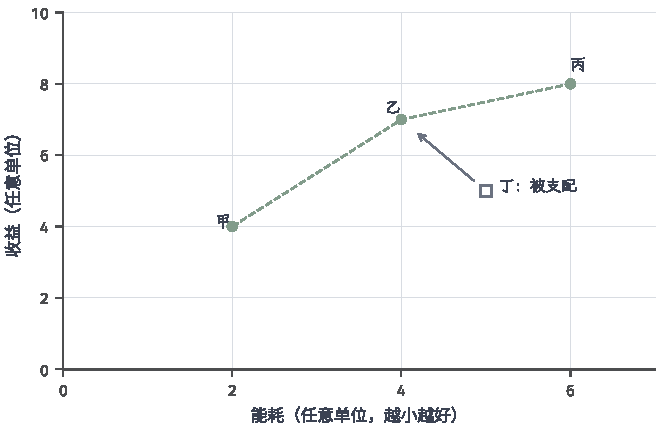
\includegraphics[width=112.000mm]{figures/10-reinforcement-learning/02-information-and-reward/matplotlib/rl-reward-pareto.pdf}
  \caption{收益越大、能耗越小越好。实心点是在四个教学候选策略中的非支配点，空心方块丁被乙支配；虚线只帮助识别候选前沿，不断言连线上的策略全部可实现。}
  \label{fig:rl-reward-pareto}
\end{figure}

据此可以区分几种看似相近的安排。预先给定偏好后求一个策略，与保留多个非支配策略供以后选择，求解的输出不同；多个来源都估计“完好交付”，则仍是同一目标的多份证据。若规定能耗必须低于上限，能耗成为不可任意用收益补偿的约束，而不只是加权分数。约束求解与执行保护由第~\ref{chap:rl-trustworthy}章展开。

% Outline: 5.4.2
\subsection{检测行为与代理奖励的偏差}
\label{sec:rl-reward-detection}

用配送代理给行为打分以前，要先检查代理是否遗漏了已知要求；策略更新以后，还要检查新行为是否超出原反馈覆盖。两种检查都需要在优化前固定独立指标、留出反馈来源和必要情形。例如按路线长度、身份字段完整性与包裹类型分层，可以主动检查训练成功轨迹中少见的情况，只从常见成功轨迹抽样则可能继续漏掉它们。

图~\ref{fig:rl-reward-overoptimization}用解析曲线演示一种待检测现象：代理分数一直上升，按独立标准衡量的行为可能先改善再恶化。两条曲线的差别提醒我们同时查看训练代理和任务证据，不说明所有训练都会遵循这个形状。真实比较还需报告指标口径、采样预算、误差范围与模型选择过程。Gao等研究了奖励模型过度优化的经验现象，本图仍是教学示意，不是该论文的测量结果\scite{gao2022overoptimization}

不同测试可以针对不同缺口。反例测试检查已有怀疑，例如照片看似送达但身份错误；压力测试增加路线长度、载荷或重复次数，考察长时交互及极端路线长度、载荷与重复运行条件。对抗测试主动寻找骗过代理的行为，例如展示别人的签收码；人工审查则分析难以形式化的失败。每次都应记录具体任务条件、行为、分数和验证器版本，使失败可以复查，不能只留下汇总总分。

如果依据留出结果调整奖励或挑选策略，这批证据就参与了开发。下一轮要补充新的独立检查，或明确报告测试复用范围，不能继续把旧结果当作未参与训练、调参与修补的测试记录上的验证。即使没有发现偏差，结论也只适用于已测情形，不能证明所有未见行为均满足要求。

\begin{figure*}[htbp]
  \centering
  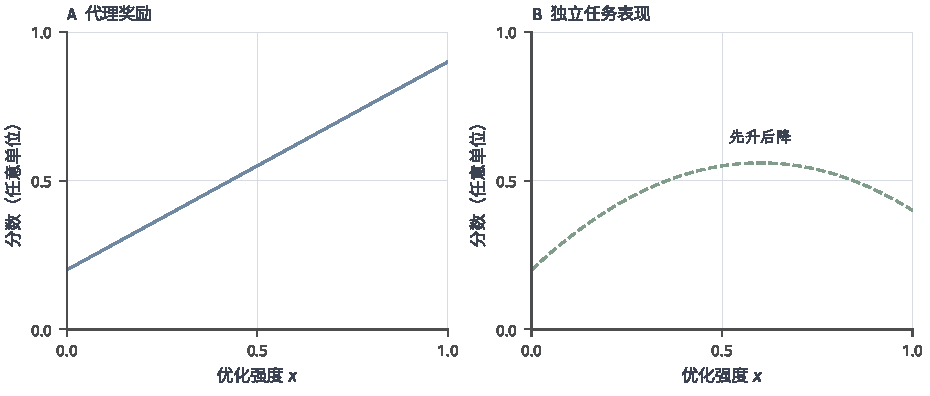
\includegraphics[width=157.400mm]{figures/10-reinforcement-learning/02-information-and-reward/matplotlib/rl-reward-overoptimization.pdf}
  \caption{代理与独立表现可能分离的双面板示意。横轴$x\in[0,1]$是归一化优化强度，曲线分别由$p(x)=0.2+0.7x$与$b(x)=0.2+1.2x-x^2$构造，纵轴为任意单位；不是实验结果，也不表示固定的普遍动力学。}
  \label{fig:rl-reward-overoptimization}
\end{figure*}

% Outline: 5.4.3
\subsection{区分奖励歧义与行为目标偏差}
\label{sec:rl-reward-ambiguity}

两个奖励都解释配送示范时，我们要继续问它们在哪些行为上等价。第~\ref{sec:rl-reward-shaping}节的势差在边界条件满足时保持所有策略的标准期望回报排序，只改变表示；另一些奖励却只在已见示范上相容，在未见路径上作出不同选择。后者限制目标外推，但要认定当前行为失配，仍需比较该行为与独立要求。

\begin{example}[示范相容不等于新路径等价]
  \label{ex:rl-reward-ambiguity}
  假设训练环境只允许专家路径$E$和路径$B$，两个终局奖励都给它们$(2,0)$，于是都支持专家选择$E$。测试环境关闭$E$，另开放此前不可行且未经专家比较的$C,D$。$R_1$给$(C,D)$的分数为$(1,-1)$，$R_2$给$(-1,1)$，而两者仍给$B$记0分。因此，对训练环境中每一条可行路径，两种奖励给出的分数相同；不同路径之间的分数并不相同。测试时两种奖励却分别支持选择$C$和$D$。即使再重复收集一万次训练选择，新增记录仍不涉及$C,D$，不能区分两种目标解释。
\end{example}

在这个例子里，原环境可用的策略可以确定，跨环境重用的奖励却不能确定。恢复原策略、解释专家奖励和恢复可迁移奖励，是强度不同的结论，第三种还要支持新选择的排序。若新状态始终没有反馈，训练得到唯一参数解也可能只是正则化或模型结构替我们作了选择，而不是示范记录识别了唯一答案。

要尝试跨环境重用奖励，一种办法是分开任务计分与依赖原环境转移规律的价值预测。\term{对抗逆强化学习}（adversarial inverse reinforcement learning, AIRL）为此将奖励项和塑形项分别参数化，再用专家与策略转移训练判别器。例如采用
\begin{equation}
  \begin{aligned}
    C(s,a,s')&=\frac{\exp f(s,a,s')}
                         {\exp f(s,a,s')+\pi(a\mid s)},\\
    f(s,a,s')&=g(s,a)+\gamma h(s')-h(s).
  \end{aligned}
  \label{eq:rl-reward-airl}
\end{equation}
其中$g$表示待恢复的奖励项，$h$表示状态上的塑形评分，$f$组合两者；$C$仍取“来自专家”的概率方向。为说明实际更新，令本轮策略$\beta=\pi^{(k)}$，用$\bm\omega$参数化$g,h$，并在式~\eqref{eq:rl-reward-airl}的分母中令$\pi=\beta$，得到$C_{\bm\omega,k}$。专家与本轮策略转移按共同的折扣和吸收协议采样，分别标为1和0。保持$\beta$固定，最大化平衡来源样本的判别对数似然
\[
  \mathcal L_C(\bm\omega)
  =\mathbb E_{\mathrm E}\log C_{\bm\omega,k}(s,a,s')
    +\mathbb E_k\log[1-C_{\bm\omega,k}(s,a,s')] .
\]
两个期望分别对应专家和本轮策略的转移分布；经验更新用各来源批次的平均替代期望，再对$\bm\omega$作梯度上升。两种来源记录的分母都使用本轮$\beta(a\mid s)$，不是在专家记录中换成专家动作概率；在所用状态动作支持上须有$\beta(a\mid s)>0$。

策略更新时冻结学出的$g,h$，原论文采用判别器的对数几率作为奖励，而非直接使用$C$或只使用$f$。由式~\eqref{eq:rl-reward-airl}可得本轮固定的信号
\[
  \widetilde r_k(s,a,s')
  =\log C_{\bm\omega,k}-\log(1-C_{\bm\omega,k})
  =f_{\bm\omega}(s,a,s')-\log\beta(a\mid s).
\]
这一等式说明判别信号包含塑形奖励及温度1的动作熵项；使用该信号时不能再重复加同一熵奖励。用本轮轨迹计算它的回报及优势估计$\widehat A_t$后，可按
$\bm\theta^{(k+1)}=\bm\theta^{(k)}
+\eta\widehat{\mathbb E}_k[
\nabla_{\bm\theta}\log\pi_{\bm\theta}(a_t\mid s_t)\widehat A_t]$
作一次策略梯度更新，梯度在旧参数处计算，$\eta>0$为步长，样本平均按本轮折扣占用加权；多步复用可采用配套的PPO等代理更新。本轮将奖励和优势视为固定，下一轮才刷新策略、转移及判别器分母，不能把冻结$\beta$的代理目标说成任意新策略下的精确熵目标。

三个数值对象可以在一条非终止转移上核算。设$g(s,a)=0.5$、$h(s)=0.2$、$h(s')=0.6$、$\gamma=0.9$，本轮动作概率$\beta(a\mid s)=0.25$。则$f=0.5+0.9(0.6)-0.2=0.84$，判别器专家概率约为$0.903$，实际策略信号为$f-\log\beta=0.84+\log4\approx2.226$。奖励分量、来源概率和训练信号数值不同；迁移讨论需要明确要带走哪个对象，而非统称“恢复奖励”。

迁移时希望重用$g$，而不是整个$f$或上述判别信号。该解释有条件：原论文的恢复分析将一般形式进一步限制为状态奖励$g(s)$，并依赖真实奖励只依赖状态、确定性动态、可分解连通条件、理想最大因果熵专家及优化等假设，且仍有允许的常数歧义。这里的连通条件是：能由同一前驱状态一步到达的两个状态视为相连，再作传递闭包，要求所有状态相连；它使当前状态项与后继状态项能够分离，而不只是要求沿路径可达。一般状态动作奖励、随机动态或有限次优示范，不会仅因写出这个分解就获得无条件恢复保证\scite{rl5-fu2018airl}

这并不意味着所有势差一换环境就失效。若保留依赖实际转移的形式
\[
  R(s,a,s')+\gamma\Phi(s')-\Phi(s),
\]
并用新环境实际后继重新计算势差，满足原边界等条件时仍可相消。若先在旧环境对后继势取期望，保存成固定状态动作奖励
$R(s,a)+\gamma\mathbb E_{T_{\mathrm{old}}}\Phi(s')-\Phi(s)$，
再直接用于新动态，旧转移期望通常不再与新轨迹上的相邻势值相消。AIRL试图区分的正是与旧动态及专家行为纠缠的部分；可否迁移需检查实际奖励形式，不能将失败归于势差本身。

旧动态期望不能直接搬用，可以用两步例子检验。起点势0，中间状态$u$势1、$v$势0，终点势0，$\gamma=0.9$。旧环境动作$A$到$u$，动作$B$到$v$，第二步都到终点；附加回报分别为$0.9+0.9(-1)=0$和0。新环境改为$A$也到$v$，若仍用旧表给$A$第一步加$0.9$，第二步在$v$加0，总和就变成$0.9$，不再与$B$相同。按新实际后继计算势差，两条路径才仍都是0。失效来自保存的旧转移期望，势差的相消形式本身没有改变。

\begin{table*}[htbp]
  \centering\small
  \begin{tabularx}{\linewidth}{@{}>{\raggedright\arraybackslash}p{25mm}*{3}{>{\raggedright\arraybackslash}X}@{}}
    \toprule
    根因 & 可观察症状 & 不能仅凭什么判断 & 补充验证 \\
    \midrule
    代理定义遗漏 & 高分行为违反未编码要求 & 训练集评分准确率 & 要求到证据审计、针对遗漏的反例 \\
    目标反馈不能区分候选奖励 & 多个相容奖励在新行为上分歧 & 奖励参数不唯一 & 有区分力的专家选择或偏好查询 \\
    反馈模型分布外误差 & 新策略行为评分与独立评价不符 & 旧分布拟合误差小 & 新行为重标、覆盖与校准检查 \\
    优化器利用漏洞 & 更新后反复产生某种虚假高分行为 & 单次异常或代理单独上涨 & 固定漏洞复现、版本对照、修补后再测 \\
    \bottomrule
  \end{tabularx}
  \caption{同一种行为偏差可能来自多个根因。奖励歧义本身不等于目标错误，唯一拟合也不能证明标准正确。}
  \label{tab:rl-reward-causes}
\end{table*}

表~\ref{tab:rl-reward-causes}将目标反馈不足、标准遗漏、分布外误差和漏洞利用分开，后两者还可能相互强化。\term{奖励投机}（reward hacking）是策略利用代理缺陷取得高分，却违反原行为要求；\term{过度优化}（overoptimization）是继续加强代理优化时，独立目标可能转而恶化。更新改变行为分布，代理在新区域评分出错，优化又偏向虚假高分行为，就可能形成这种反馈。不过分布外误差未必已被利用，奖励不唯一也未必造成错误行为，仍要用具体反例和独立要求作判断。

% Outline: 5.4.4
\subsection{修订行为目标并约束策略更新}
\label{sec:rl-reward-revision}

发现高分配送有问题后，需要按根因选择修订对象。新增“内部完好”要求，是补充原目标；为同一完好标准补充标签说明，是修订操作性标注规则。重训评分器改进对既定标准的估计，修补允许空字符串通过的验证器则修正实现。四种改动影响不同，必须保留目标、标注、验证器和策略版本，不能统称为奖励模型升级。

修订以后若仍有估计误差，可以惩罚可估计的模型不确定性，用多个奖励模型的分歧定位缺口，或限制策略更新幅度。这些措施各有边界：模型可能共享盲点，不确定性估计也可能失准；保守更新减少进入未见区域的速度，同时可能压低原本可获得的收益。KL约束只控制相对参考策略的偏移，不能补回参考策略已遗漏的要求，平均KL小也不保证每个罕见状态都不变。

新增反例及反馈训练记录应回答已经发现的缺口。例如旧签收照片骗过代理时，可以补充照片与当前包裹身份的一致性检查，再收集不同伪造变体。模型刷新后重测原反例，并检查未参与修补的新变体，才能判断修订是否扩大了正确覆盖。比较时还要记录独立任务指标的变化、采用保守更新后减少的任务收益以及新增反馈成本，不能只报告旧训练集拟合改善。

图~\ref{fig:rl-reward-revision}显示不同修订如何返回检测：目标改动要重新明确要求，估计或实现改动要重新检验新行为。关闭一个反例不表示其他要求都已满足；风险、约束违反和运行时保护还需要第~\ref{chap:rl-trustworthy}章的工具。

\begin{figure*}[htbp]
  \centering
  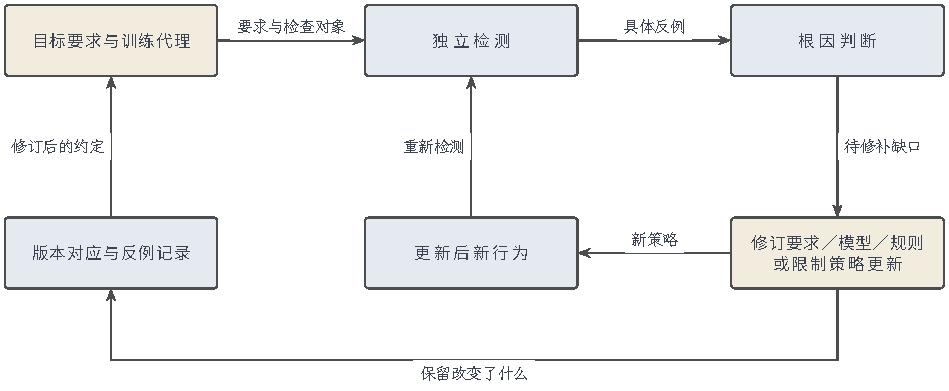
\includegraphics[width=160.616mm]{figures/10-reinforcement-learning/02-information-and-reward/tikz/rl-reward-revision.pdf}
  \caption{目标与代理的诊断回路。检测传递具体反例，根因判断决定改变要求、修订估计还是限制更新；修订后的策略产生新行为，必须重新接受独立检测。}
  \label{fig:rl-reward-revision}
\end{figure*}

% Outline: 5.5
\section{三类奖励限制叠加时的反馈学习}
\label{sec:rl-reward-loop}

真实的配送训练往往同时面临三类限制：只有少量示范、部分路线偏好、若干过程记录，加上一个并不完备的验证器。可以把这些材料组织成一轮可复查的学习闭环：先明确本轮的行为要求与每条反馈的用途，再据此更新有依据的模型或策略，然后用独立证据检验新行为，最后决定是停止还是追加反馈查询。只有在这个闭环里，各步骤才有真实的先后依赖；三类限制本身提供的是不同的诊断依据，并不要求每轮把它们依次消除。如果某种要求始终没有任何反馈涉及，再多次迭代也无法自动解除目标上的歧义。

% Outline: 5.5.1
\subsection{整合已有反馈形成当前反馈约束}
\label{sec:rl-reward-integration}

将配送示范、偏好和检查记录放在一起以前，需要知道它们各自在评价什么。一条可用记录至少包含任务指令与配送条件、被评价行为、反馈值和形式、来源、采样策略及标准版本。轨迹评分还要记录步骤范围和终止原因，偏好还要保留两个候选及呈现顺序。这些字段使我们能够区分冲突来自行为条件、评分尺度还是标准变化。

这里用“反馈约束”概括记录对候选行为和评价模型提供的限制，但实施时必须分开三件事。行为要求规定什么算完成任务，例如交给正确收件人；训练目标规定怎样利用记录拟合模型，例如动作负对数似然和偏好比较损失。策略更新限制则规定本轮允许多大偏移，或排除哪些行为。带噪偏好通常进入损失，不是每条都必须满足的硬不等式；身份要求若作为硬约束，还要有可检查条件和可靠执行机制。

表~\ref{tab:rl-reward-records}按记录、约束对象和本轮用途整合配送反馈。同一批反馈记录可以支持多个模型，但动作标签、相对排序和正确性判断的语义不同，在说明聚合依据前不能直接相加成总分。

\begin{table*}[htbp]
  \centering\small
  \begin{tabularx}{\linewidth}{@{}*{5}{>{\raggedright\arraybackslash}X}@{}}
    \toprule
    反馈记录 & 约束对象 & 可靠范围 & 冲突处理 & 本轮用途 \\
    \midrule
    专家装载动作 & 条件动作分布 & 指令完整的已见状态 & 检查隐含指令与次优示范 & 行为克隆初始化或局部纠正 \\
    同包裹路线偏好 & 相对效用 & 同一偏好群体与标准 & 保留来源分层，不强行平均 & 拟合路线效用差 \\
    装载身份检查 & 步骤关系正确性 & 可读编号且检查器有效 & 与终点身份联合复核 & 提供局部信号 \\
    签收验证 & 最终身份条件 & 签收记录可信 & 排除旧记录与解析漏洞 & 终局反馈；另留独立样本 \\
    少量完好评分 & 包裹状态评价 & 评分尺度一致 & 复核尺度与开箱依据 & 校准反馈模型 \\
    独立开箱审查 & 未覆盖要求的证据 & 被抽查任务范围 & 不用于本轮拟合 & 检查代理遗漏 \\
    \bottomrule
  \end{tabularx}
  \caption{同一轮反馈记录的五项对应。独立证据应按样本和用途隔离，不能一边参与拟合一边称为留出检验。}
  \label{tab:rl-reward-records}
\end{table*}

假设专家走楼梯，偏好却选择电梯。先比较包裹是否易碎、当时电梯是否可用、评价者是否强调节能；只有条件和标准相同时，才需要进一步判断来源可靠性或专家是否次优。装载检查通过而终局身份失败，也可能来自中途换包，局部标签各自都正确，但跨步骤一致性被破坏。保留条件和粒度才能定位这些差异，平均正负分反而可能掩盖原因。

整合后，本轮要确定明确的要求、训练目标和更新限制。例如先要求身份正确，再在满足身份条件的行为中比较完好与能耗；用动作示范拟合策略，用路线偏好和完好评分分别拟合比较模型及评分模型。策略更新还可以采用参考KL惩罚或约束，但必须说明是哪一种。身份优先的文字约定并没有自动提供动作过滤器，硬性执行能力仍要验证。所有约定都应附上适用任务条件与可得观测范围及尚未解决的分歧。

若分歧确实来自不能兼容的真实偏好，可以保留按偏好条件选择的策略或多个候选。必须聚合时，应解释分数单位、尺度、权重及权重代表的取舍；加权平均是一个新约定，不是争议已经被识别为唯一真实目标的证据。

% Outline: 5.5.2
\subsection{依据反馈约束联合更新模型与策略}
\label{sec:rl-reward-joint-update}

已有反馈及其用途确定后，要明确本轮改动哪些学习对象。对应记录可用于拟合奖励、效用或通过概率模型，归因机制再把轨迹结果转成局部信号，策略在本轮惩罚或约束下利用这些信号更新，并产生下一批行为。价值基线帮助降低方差或自举，不替代已经约定的行为评价标准。“联合更新”可以是交替拟合，也可以只改其中一项，不要求全部参数同时反向传播。图~\ref{fig:rl-reward-update}标明反馈记录、归因结果与参数更新之间的依赖，以及本轮冻结的标准和参考策略。

\begin{figure*}[htbp]
  \centering
  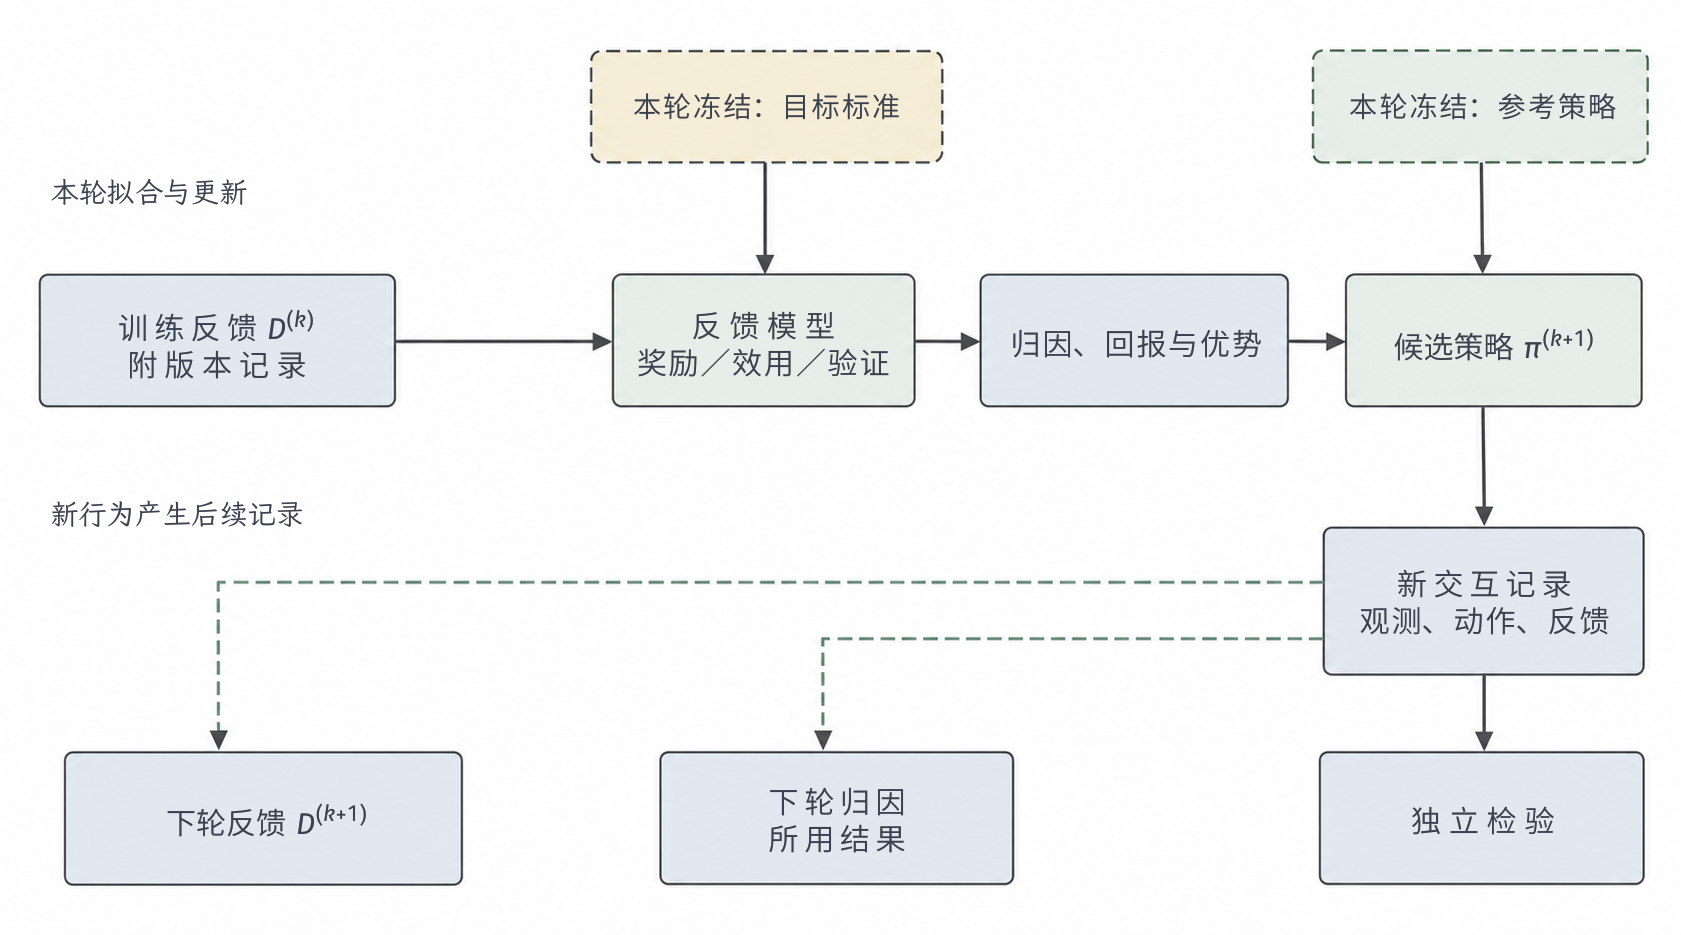
\includegraphics[width=157.400mm]{figures/10-reinforcement-learning/02-information-and-reward/generated/rl-reward-update/figure.png}
  \caption{本轮更新及下一轮补充的记录依赖。实线表示从本轮训练反馈形成反馈模型、局部信号和候选策略的依赖；候选策略产生的新交互记录，沿虚线回流箭头进入下一轮的反馈整合或归因。虚线框表示本轮冻结的目标标准和参考策略。独立检验记录不回流本轮拟合。}
  \label{fig:rl-reward-update}
\end{figure*}

在这条更新路径中，反馈来源和优化器是两个选择。RLHF与RLAIF可以采用相同策略优化器而使用不同评价者；迭代式偏好优化可以每轮补新偏好，再运行DPO；在线RLVR则对当前策略样本即时调用规则验证。\term{解耦剪裁与动态采样策略优化}（Decoupled Clip and Dynamic sAmpling Policy Optimization, DAPO）是其中一种具体更新方法。表~\ref{tab:rl-reward-loops}比较各轮更新和固定的对象，以及样本和反馈何时刷新，而不是将这些名称当成互斥算法类别。

\begin{table*}[htbp]
  \centering\small
  \begin{tabularx}{\linewidth}{@{}>{\raggedright\arraybackslash}p{23mm}*{3}{>{\raggedright\arraybackslash}X}@{}}
    \toprule
    路线 & 本轮更新对象 & 本轮固定对象 & 采样与反馈刷新 \\
    \midrule
    PPO式RLHF & 奖励模型、策略及价值可分阶段更新 & 标注标准、参考策略；策略阶段冻结奖励 & 当前策略采样，按预算补人类偏好 \\
    RLAIF & 反馈模型与策略，依实现可有价值模型 & AI评价模型、提示与标准的指定版本 & 新样本交由AI评价，独立抽查 \\
    迭代式偏好优化 & 偏好对上的策略参数 & 单轮偏好集与参考策略 & 外层采样和标注刷新，内层可离线DPO \\
    在线RLVR & 策略；基线依更新器而定 & 验证规则、参考答案或程序测试用例 & 新策略候选逐批验证 \\
    DAPO & 无独立评论家的策略更新 & 当前验证规则、旧策略批次概率 & 动态采样补充混合得分组，按token聚合损失 \\
    \bottomrule
  \end{tabularx}
  \caption{反馈闭环而非互斥算法分类。DAPO是在线可验证反馈的一种具体实现，RLAIF也可以组合不同的策略优化器。}
  \label{tab:rl-reward-loops}
\end{table*}

表中的DAPO修改集中在剪裁、样本筛选和损失聚合。它在所讨论训练设置中使用规则结果奖励，去掉参考KL项，采用不同的上下剪裁阈值，并动态补充组内同时产生成功和失败回答的任务提示。损失还从式~\eqref{eq:rl-reward-grpo}的回答内平均，改为对全部有效token平均。为比较长度权重，记剪裁项为$\ell_{i,t}$，两种聚合是
\begin{equation}
  \frac1m\sum_i\frac1{T_i}\sum_t\ell_{i,t},
  \qquad
  \frac1{\sum_iT_i}\sum_i\sum_t\ell_{i,t}.
  \label{eq:rl-reward-dapo-weight}
\end{equation}
前者赋予每个回答相同总权重，后者赋予每个token相同权重，使长回答在整批损失中占更大总权重。超长惩罚与截断处理也会改变反馈语义；论文称之为reward shaping，不意味着满足本章的潜势型不变条件。DAPO发表于NeurIPS 2025，但经验结果只对应报告中的模型、数学任务和预算，不能推出这些组件对所有任务都有收益\scite{rl5-yu2025dapo}

长度聚合的差别可以在两个回答上直接算出。令长度为2和4，各token剪裁项分别为1和$-1$。先各回答平均再平均，值为$(1-1)/2=0$；对全部token平均则为$(2-4)/6=-1/3$。前者让两回答总权重相同，后者让较长的负项回答占更多权重。两个代理数值只是权重差的示例，不表示真实任务回报也发生了同样幅度的变化。

动态采样补混合得分组，可以减少零相对信号，但筛选也改变被选入训练的任务提示分布，被丢弃候选仍消耗采样和验证预算。过滤整组失败的困难题，没有解决这些题。提高剪裁上界只是改变代理目标梯度何时饱和，不是对动作概率施加硬上限。因而比较实现时，应同时记录样本选择、组内标准差分母、长度聚合方式和验证器版本。

\begin{example}[一轮可复查的更新记录]
  \label{ex:rl-reward-round}
  假设教学轮次$k=3$使用训练反馈记录$D^{(3)}$、身份与完好标准$\texttt{std-2}$、反馈模型$\texttt{feedback-3}$、旧策略$\pi^{(3)}$和参考策略$\pi_{\mathrm{ref}}$。$D^{(3)}$有20条装载动作、12对偏好、8条完好评分，分别用于策略拟合、比较模型拟合和评分模型拟合，后两项组成$\texttt{feedback-3}$。策略更新时冻结$\texttt{std-2},\texttt{feedback-3},\pi_{\mathrm{ref}}$，独立审查记录不加入$D^{(3)}$。

  再取两条等长四步轨迹，以本轮约定的综合代理$\widetilde R$给终局记1和0分，中间奖励为零，$\gamma=0.9$，于是起点回报为$0.729$和0。冻结基线为$0.3645$，减去基线得到样本优势$0.3645$和$-0.3645$。只更新起点二动作的logit，其他动作规则固定；初始logit为0，两条轨迹各来自一个起点动作，样本平均梯度为$0.18225$。令步长为$0.2$、KL系数为$0.1$，且当前策略恰与参考相同，精确KL梯度此时为零。一次未剪裁更新得到logit $0.03645$，正优势动作概率约为$0.5091$，作为候选$\pi^{(4)}$。

  本轮记录目标为“轨迹代理回报的PPO式改进减参考KL”，并分别预留40个访问状态动作标签、20对比较、100次验证和10次人工审查的预算上限。更新后要分开检验$\texttt{feedback-3}$是否更符合反馈和$\pi^{(4)}$是否改善实际行为。这些计算是可复查的教学记录，不是实际测得的任务回报。
\end{example}

% Outline: 5.5.3
\subsection{用更新后行为检验反馈约束的有效性}
\label{sec:rl-reward-loop-check}

候选$\pi^{(4)}$产生新行为后，要按本轮开始前的标准检查，不能只重算$\pi^{(3)}$的旧日志分数。三类限制分别对应三个问题：新状态是否超出反馈覆盖，局部信号是否仍正确联系关键动作与结果，代理回报增加时独立行为指标是否改善。表~\ref{tab:rl-reward-checks}分列相应证据和失效判据，使一种检查通过不能替代其他检查。

\begin{table*}[htbp]
  \centering\small
  \begin{tabularx}{\linewidth}{@{}>{\raggedright\arraybackslash}p{20mm}*{4}{>{\raggedright\arraybackslash}X}@{}}
    \toprule
    检查 & 待检查行为与任务条件 & 独立证据 & 失效判据 & 仍未覆盖范围 \\
    \midrule
    观测与覆盖 & 新策略访问状态、长短轨迹 & 新状态专家标签、留出来源评分 & 无支持区域仍被赋予高置信评价 & 未覆盖的任务条件和状态动作 \\
    局部归因 & 关键步骤与相关标记 & 受控扰动、过程复核、终局结果 & 无关标记改变信号，关键错误不受罚 & 不可干预步骤的因果贡献 \\
    目标匹配 & 代理高分的新行为 & 独立身份、完好和成本检查 & 违反已约定要求或独立指标退化 & 未形式化与难观测要求 \\
    来源一致性 & 同行为的多来源判断 & 第三方执行或事实核对 & 分歧无法由条件差异解释 & 一致来源的共同盲点 \\
    \bottomrule
  \end{tabularx}
  \caption{检验必须说明未覆盖范围。来源一致性可以暴露冲突，却不能替代外部事实证据。}
  \label{tab:rl-reward-checks}
\end{table*}

检验结果应区分证据支持、证据不足和明确失效。若$\pi^{(4)}$在预定短路线、身份可读范围内完成全部检查，估计精度也达到事先要求，可以支持当前反馈在这个范围有效。若只测三次且均成功，仍未覆盖必要长路线或满足精度要求，就只能说暂未发现失败。若已有代理高分却交错收件人的行为，便得到明确反例；平均成功率高不能抹去这个失效。

暂未看见失败也可能只是样本少。假设固定策略在同一测试条件下每次独立有$0.1$错误率，三次都通过的概率仍为$0.9^3=0.729$。因此“三次通过”在这样的策略下很常见，不能单独证明错误率很低。这个概率不是看到三次通过后的错误率后验；它说明接受结论还需事先约定的统计精度和覆盖依据。

诊断要返回对应缺口：新状态无标签就补访问覆盖，关键步骤局部信号错误就修订归因，完好要求未编码就修订标准或代理。这样可以针对已有证据改变相关对象，不必一次失败就重训全部模型。反例若进入下一轮修订，就成为开发记录，后续不能再将它单独称为独立留出检验。

% Outline: 5.5.4
\subsection{依据检验结果与反馈预算决定停止或继续}
\label{sec:rl-reward-stopping}

即使新行为全部通过已做检查，也需要判断检查是否达到了事先约定的要求。训练前应固定独立指标的接受标准、必要覆盖、统计精度或不确定性要求，以及各类预算上限，不能看到结果后再放宽门槛。有限测试可以支持限定范围的接受，不为未测范围提供“没有失败”的保证。

\begin{table*}[htbp]
  \centering\small
  \begin{tabularx}{\linewidth}{@{}>{\raggedright\arraybackslash}p{23mm}*{3}{>{\raggedright\arraybackslash}X}@{}}
    \toprule
    证据状态 & 允许的后续动作 & 必须保留的结论范围 & 所需反馈或检查记录 \\
    \midrule
    达到预设充分性与接受标准 & 停止训练，保留复核入口 & 只接受已测任务、标准和策略版本 & 已完成覆盖、精度及成本记录 \\
    未发现失败但证据不足 & 有预算则定向查询；否则停止或收窄范围 & 未证实原范围满足要求；预算停止不等于成功 & 缺少的场景、样本或独立来源 \\
    已发现明确失效 & 暂停对该范围的接受，修订后再测；或终止 & 记录反例与不适用范围 & 根因、修补方案、验证与查询成本 \\
    \bottomrule
  \end{tabularx}
  \caption{停止训练是一种行动，接受行为是一个证据结论，二者不能混同。}
  \label{tab:rl-reward-stopping}
\end{table*}

表~\ref{tab:rl-reward-stopping}区分停止行动和接受结论。满足预设要求可以停止，预算耗尽也可以停止，但后者仍可能留有关键缺口。若获准查询只能看终点照片，不能观察包裹内部，重复评价也无法识别完好要求；这时应收窄结论或改变反馈可读取的字段或查询权限，而不是将次数当作充分性。

有剩余预算时，还要说明下一批反馈可能改善哪项判断：当前状态覆盖、候选目标排序、过程贡献或验证规则。可以估计查询减少多少候选模型分歧、是否可能改变决策，再与人工时间、采样和执行成本比较；没有用于校准查询收益估计的已有记录时，这些只是启发式依据，不是有数值保证的查询后决策收益。更换目标、反馈标准或明显改变策略访问分布后，原停止证据所对应的对象也变了，需要重新检查。

\begin{algorithm}[反馈学习的继续与停止闭环]
  \label{alg:rl-reward-loop}
  \begin{algorithmic}[1]
    \Require 目标标准、独立接受条件、必要覆盖、分项预算、初始反馈与策略
    \Ensure 候选策略、结论范围、停止原因和未解决缺口
    \While{尚未记录停止原因}
      \State 整合兼容的反馈，固定本轮标准、本轮训练反馈记录的范围及未解决分歧
      \State 只更新有相应证据支持的反馈模型、归因机制或策略
      \State 以新行为接受独立检查，分类为充分、证据不足或明确失效
      \If{覆盖与精度充分，且满足预设接受条件}
        \State 记录“在已检验范围满足要求”，停止本轮学习
      \ElsIf{预算不足，或允许查询不能区分关键目标解释}
        \State 记录“预算停止”或“识别受限”，收窄结论并停止
      \Else
        \State 按观测、归因或目标缺口选查询，必要时先修订目标标准
        \State 获取新反馈，记录成本、生成策略与标准版本，返回整合
      \EndIf
    \EndWhile
  \end{algorithmic}
\end{algorithm}

算法~\ref{alg:rl-reward-loop}只更新有相应证据支持的对象，不要求每轮全部模型变化。明确失效可能先需要修订要求，而不是马上增加样本；若获准查询无法补足缺口，也可以停止优化错误代理，并保留未解决结论。这个规则控制反馈学习是否继续，不替代系统部署审批或运行流程。

% Outline: 5.5.5
\subsection{针对反馈缺口获取新反馈}
\label{sec:rl-reward-query}

决定继续后，还需把未决问题转成可执行查询。例如错误走廊缺恢复动作，就查询该状态上的专家标签；两条新路线排序不定，就比较候选奖励意见不同的路线。表~\ref{tab:rl-reward-queries}按这类缺口列出查询能排除的解释，同时保留查询之后仍未回答的部分。

\begin{table*}[htbp]
  \centering\small
  \begin{tabularx}{\linewidth}{@{}*{4}{>{\raggedright\arraybackslash}X}@{}}
    \toprule
    具体缺口 & 查询方式 & 可以排除的解释 & 仍不能回答什么 \\
    \midrule
    偏离后不会恢复 & 当前访问状态上的专家动作 & 这些状态上的错误动作候选 & 唯一真实奖励与未查询状态 \\
    新路径排序不确定 & 比较奖励候选意见不同的路径 & 对该比较给出相反排序的目标 & 其他任务条件或评价群体的偏好 \\
    关键过程贡献不清 & 步骤标注、受控检查与结果对照 & 局部无效却被奖励的归因 & 未控制混杂下的完整因果结构 \\
    验证标准遗漏 & 新结果检查、规则边界与对抗案例 & 会接受已知错误行为的验证器 & 未被形式化的全部要求 \\
    来源共同偏差 & 独立来源和实际执行审查 & 仅依赖共同代理的解释 & 未审查行为的真实性 \\
    \bottomrule
  \end{tabularx}
  \caption{查询应取得能区分候选奖励或反馈模型的评价结果，而不只是重复已经一致的反馈。}
  \label{tab:rl-reward-queries}
\end{table*}

可回接前面的新路径歧义：两个奖励都给训练路径$E,B$相同分数，再比较这两条路径不会区分它们；两奖励对$C,D$却给相反排序。针对$C,D$取得同条件、同评价标准的比较，才可能提供新的区分证据。若反馈有噪声，还需控制误排序，而不能把一次回答当作排除所有其他解释。查询的价值在于回答未决问题，不在于再增加一条已经一致的标签。

查询的选择依据也不同。DAgger查询当前访问状态的专家动作，主动偏好查询选择可能改变候选排序的比较；不确定性采样选择反馈模型分歧大的行为，在线验证检查当前策略产物，对抗收集则寻找代理漏洞。但模型分歧的大小未必反映新反馈对真实行为要求的区分程度：共同盲点可能让模型一致自信，模糊措辞却可能造成很大分歧而不改变行为要求。保留独立随机或分层抽查，可以检查主动筛选是否遗漏重要区域。

沿示例~\ref{ex:rl-reward-round}，假设$\pi^{(4)}$主要缺恢复动作，可以查询6个实际访问状态的动作；为新路线再补4对偏好、24次验证和2次人工审查。还要分别记录取得候选所用轨迹数及环境步数。这些教学计数单位不同，相加成“36条反馈”不能说明成本；每批记录应附带生成策略$\pi^{(4)}$、标准$\texttt{std-2}$及采样筛选协议。

新反馈返回第~\ref{sec:rl-reward-integration}节时，先核对与旧标准的兼容性。沿用$\texttt{std-2}$的记录可聚合；若$\texttt{std-3}$新增内部破损要求，旧终点照片标签只支持原先被检查的条件，需视用途重标或分开使用，不能直接当作$\texttt{std-3}$的完整正例。若全部获准查询只比较速度，就仍无法区分看重完好和看重能耗的目标解释。此时应报告识别边界，闭环轮数没有补足区分这些目标解释所需的评价记录。

% Outline: 5.6
\section{本章小结}
\label{sec:rl-reward-summary}

回到配送中的反馈缺口，替代记录首先决定我们能学到什么。示范约束动作或长期占用，评分和偏好约束评价函数，验证只判断明示条件；它们不相互等价，也不必都先还原为唯一奖励。BC在已有专家分布上拟合，DAgger补当前访问状态；奖励模型加策略优化需要评分新行为，标准DPO拟合固定偏好对。GRPO怎样比较组内候选，则与分数是否来自规则是两个选择。

取得结果以后，还要判断它怎样支持早期动作更新。结果回溯重新记账，过程监督增加证据，奖励变换和辅助目标改变信号或训练位置，各有成本与保持条件。潜势塑形在有界势、共同初始分布及正确终端处理下，靠相邻势项相消保持标准期望回报排序；这不证明局部信号具有因果意义，也不保证风险排序或学习速度不变。

最后，训练信号是否表达行为要求，要用独立证据检验。反馈拟合准确不证明标准完整，相容奖励也可能在未比较行为上分歧；它们若一致支持当前策略，结论也应保留相应范围。每轮反馈学习都要固定标准、更新对象和检验证据，再取得能补具体缺口的新反馈。停止时说明是已在限定范围满足要求、预算耗尽，还是允许的查询仍无法识别关键目标。

